\PassOptionsToPackage{unicode=true}{hyperref} % options for packages loaded elsewhere
\PassOptionsToPackage{hyphens}{url}
%
\documentclass[]{book}
\usepackage{lmodern}
\usepackage{amssymb,amsmath}
\usepackage{ifxetex,ifluatex}
\usepackage{fixltx2e} % provides \textsubscript
\ifnum 0\ifxetex 1\fi\ifluatex 1\fi=0 % if pdftex
  \usepackage[T1]{fontenc}
  \usepackage[utf8]{inputenc}
  \usepackage{textcomp} % provides euro and other symbols
\else % if luatex or xelatex
  \usepackage{unicode-math}
  \defaultfontfeatures{Ligatures=TeX,Scale=MatchLowercase}
\fi
% use upquote if available, for straight quotes in verbatim environments
\IfFileExists{upquote.sty}{\usepackage{upquote}}{}
% use microtype if available
\IfFileExists{microtype.sty}{%
\usepackage[]{microtype}
\UseMicrotypeSet[protrusion]{basicmath} % disable protrusion for tt fonts
}{}
\IfFileExists{parskip.sty}{%
\usepackage{parskip}
}{% else
\setlength{\parindent}{0pt}
\setlength{\parskip}{6pt plus 2pt minus 1pt}
}
\usepackage{hyperref}
\hypersetup{
            pdftitle={Foundational Statistics - Bi 610 - Spring 2020},
            pdfauthor={Clayton M. Small and William A. Cresko},
            pdfborder={0 0 0},
            breaklinks=true}
\urlstyle{same}  % don't use monospace font for urls
\usepackage{color}
\usepackage{fancyvrb}
\newcommand{\VerbBar}{|}
\newcommand{\VERB}{\Verb[commandchars=\\\{\}]}
\DefineVerbatimEnvironment{Highlighting}{Verbatim}{commandchars=\\\{\}}
% Add ',fontsize=\small' for more characters per line
\usepackage{framed}
\definecolor{shadecolor}{RGB}{248,248,248}
\newenvironment{Shaded}{\begin{snugshade}}{\end{snugshade}}
\newcommand{\AlertTok}[1]{\textcolor[rgb]{0.94,0.16,0.16}{#1}}
\newcommand{\AnnotationTok}[1]{\textcolor[rgb]{0.56,0.35,0.01}{\textbf{\textit{#1}}}}
\newcommand{\AttributeTok}[1]{\textcolor[rgb]{0.77,0.63,0.00}{#1}}
\newcommand{\BaseNTok}[1]{\textcolor[rgb]{0.00,0.00,0.81}{#1}}
\newcommand{\BuiltInTok}[1]{#1}
\newcommand{\CharTok}[1]{\textcolor[rgb]{0.31,0.60,0.02}{#1}}
\newcommand{\CommentTok}[1]{\textcolor[rgb]{0.56,0.35,0.01}{\textit{#1}}}
\newcommand{\CommentVarTok}[1]{\textcolor[rgb]{0.56,0.35,0.01}{\textbf{\textit{#1}}}}
\newcommand{\ConstantTok}[1]{\textcolor[rgb]{0.00,0.00,0.00}{#1}}
\newcommand{\ControlFlowTok}[1]{\textcolor[rgb]{0.13,0.29,0.53}{\textbf{#1}}}
\newcommand{\DataTypeTok}[1]{\textcolor[rgb]{0.13,0.29,0.53}{#1}}
\newcommand{\DecValTok}[1]{\textcolor[rgb]{0.00,0.00,0.81}{#1}}
\newcommand{\DocumentationTok}[1]{\textcolor[rgb]{0.56,0.35,0.01}{\textbf{\textit{#1}}}}
\newcommand{\ErrorTok}[1]{\textcolor[rgb]{0.64,0.00,0.00}{\textbf{#1}}}
\newcommand{\ExtensionTok}[1]{#1}
\newcommand{\FloatTok}[1]{\textcolor[rgb]{0.00,0.00,0.81}{#1}}
\newcommand{\FunctionTok}[1]{\textcolor[rgb]{0.00,0.00,0.00}{#1}}
\newcommand{\ImportTok}[1]{#1}
\newcommand{\InformationTok}[1]{\textcolor[rgb]{0.56,0.35,0.01}{\textbf{\textit{#1}}}}
\newcommand{\KeywordTok}[1]{\textcolor[rgb]{0.13,0.29,0.53}{\textbf{#1}}}
\newcommand{\NormalTok}[1]{#1}
\newcommand{\OperatorTok}[1]{\textcolor[rgb]{0.81,0.36,0.00}{\textbf{#1}}}
\newcommand{\OtherTok}[1]{\textcolor[rgb]{0.56,0.35,0.01}{#1}}
\newcommand{\PreprocessorTok}[1]{\textcolor[rgb]{0.56,0.35,0.01}{\textit{#1}}}
\newcommand{\RegionMarkerTok}[1]{#1}
\newcommand{\SpecialCharTok}[1]{\textcolor[rgb]{0.00,0.00,0.00}{#1}}
\newcommand{\SpecialStringTok}[1]{\textcolor[rgb]{0.31,0.60,0.02}{#1}}
\newcommand{\StringTok}[1]{\textcolor[rgb]{0.31,0.60,0.02}{#1}}
\newcommand{\VariableTok}[1]{\textcolor[rgb]{0.00,0.00,0.00}{#1}}
\newcommand{\VerbatimStringTok}[1]{\textcolor[rgb]{0.31,0.60,0.02}{#1}}
\newcommand{\WarningTok}[1]{\textcolor[rgb]{0.56,0.35,0.01}{\textbf{\textit{#1}}}}
\usepackage{longtable,booktabs}
% Fix footnotes in tables (requires footnote package)
\IfFileExists{footnote.sty}{\usepackage{footnote}\makesavenoteenv{longtable}}{}
\usepackage{graphicx,grffile}
\makeatletter
\def\maxwidth{\ifdim\Gin@nat@width>\linewidth\linewidth\else\Gin@nat@width\fi}
\def\maxheight{\ifdim\Gin@nat@height>\textheight\textheight\else\Gin@nat@height\fi}
\makeatother
% Scale images if necessary, so that they will not overflow the page
% margins by default, and it is still possible to overwrite the defaults
% using explicit options in \includegraphics[width, height, ...]{}
\setkeys{Gin}{width=\maxwidth,height=\maxheight,keepaspectratio}
\setlength{\emergencystretch}{3em}  % prevent overfull lines
\providecommand{\tightlist}{%
  \setlength{\itemsep}{0pt}\setlength{\parskip}{0pt}}
\setcounter{secnumdepth}{5}
% Redefines (sub)paragraphs to behave more like sections
\ifx\paragraph\undefined\else
\let\oldparagraph\paragraph
\renewcommand{\paragraph}[1]{\oldparagraph{#1}\mbox{}}
\fi
\ifx\subparagraph\undefined\else
\let\oldsubparagraph\subparagraph
\renewcommand{\subparagraph}[1]{\oldsubparagraph{#1}\mbox{}}
\fi

% set default figure placement to htbp
\makeatletter
\def\fps@figure{htbp}
\makeatother

\usepackage{booktabs}
\usepackage{amsthm}
\makeatletter
\def\thm@space@setup{%
  \thm@preskip=8pt plus 2pt minus 4pt
  \thm@postskip=\thm@preskip
}
\makeatother
\usepackage[]{natbib}
\bibliographystyle{apalike}

\title{Foundational Statistics - Bi 610 - Spring 2020}
\author{Clayton M. Small and William A. Cresko}
\date{2020-04-30}

\begin{document}
\maketitle

{
\setcounter{tocdepth}{1}
\tableofcontents
}
\hypertarget{course-overview}{%
\chapter{Course Overview}\label{course-overview}}

This is the complete set of \emph{course materials} for the \emph{Foundational Statistics Course} at the University of Oregon for the Spring of 2020. It is written in \textbf{Markdown} so that it can be easily updated.

In this book you will find nearly all the information you will need to complete the course.

\hypertarget{introduction-to-the-course}{%
\chapter{Introduction to the course}\label{introduction-to-the-course}}

This is the complete set of \emph{course materials} for the \emph{Foundational Statistics Course} at the University of Oregon for the Spring of 2020. It is written in \textbf{Markdown} so that it can be easily updated.

In this book you will find nearly all the information you will need to complete the course.

\hypertarget{instructors}{%
\section{Instructors}\label{instructors}}

Dr.~Clay Small, \href{mailto:csmall@uoregon.edu}{\nolinkurl{csmall@uoregon.edu}}

Dr.~Bill Cresko, \href{mailto:wcresko@uoregon.edu}{\nolinkurl{wcresko@uoregon.edu}}

\hypertarget{course-information}{%
\section{Course Information}\label{course-information}}

Virtual Office Hours: T-R 12 to 1:30 (Zoom)

\hypertarget{software}{%
\section{Software}\label{software}}

\begin{itemize}
\item
  Latest version of R
\item
  Latest version of RStudio
\end{itemize}

\hypertarget{inclusion-and-accessibility}{%
\section{Inclusion and Accessibility}\label{inclusion-and-accessibility}}

Please tell us your preferred pronouns and/or name, especially if it differs from the class roster. We take seriously our responsibility to create inclusive learning environments. Please notify us if there are aspects of the instruction or design of this course that result in barriers to your participation! You are also encouraged to contact the Accessible Education Center in 164 Oregon Hall at 541-346-1155 or \href{mailto:uoaec@uoregon.edu}{\nolinkurl{uoaec@uoregon.edu}}.

We are committed to making this course an inclusive and respectful learning space. Being respectful includes using preferred pronouns for your classmates. Your classmates come from a diverse set of backgrounds and experiences; please avoid assumptions or stereotypes, and aim for inclusivity. Let us know if there are classroom dynamics that impede your (or someone else's) full engagement.

Because of the COVID-19 pandemic, this course is being delivered entirely remotely. We realized that this situation makes it difficult for some students to interact with the material, for a variety of reasons. We are committed to flexibility during this stressful time and emphasize that we will work with students to overcome difficult barriers as they arise.

Please see this page for more information on campus resources, academic integrity, discrimination, and harassment (and reporting of it).

\hypertarget{course-schedule}{%
\chapter{Course Schedule}\label{course-schedule}}

\hypertarget{weeks-1-2}{%
\section{Weeks 1-2}\label{weeks-1-2}}

\begin{enumerate}
\def\labelenumi{\arabic{enumi}.}
\tightlist
\item
  Data organization and management

  \begin{itemize}
  \tightlist
  \item
    best practices, reproducibility, etc.
  \end{itemize}
\item
  Basic programming fundamentals for data curation

  \begin{itemize}
  \tightlist
  \item
    The Unix environment and fundamental commands
  \item
    Formatting and manipulating tabular text files from the terminal
  \end{itemize}
\item
  Introduction to R and Rstudio

  \begin{itemize}
  \tightlist
  \item
    Installation/Updates
  \item
    R object types and assignment
  \end{itemize}
\item
  Practice with R objects

  \begin{itemize}
  \tightlist
  \item
    vectors, matrices, data frames, etc.
  \end{itemize}
\item
  Applying core programming fundamentals in R

  \begin{itemize}
  \tightlist
  \item
    vectorized operations
  \item
    replicate, apply family, ifelse, for loops, etc.
  \end{itemize}
\end{enumerate}

\hypertarget{week-3}{%
\section{Week 3}\label{week-3}}

\begin{enumerate}
\def\labelenumi{\arabic{enumi}.}
\tightlist
\item
  Plotting/visualizing data as a means of exploration

  \begin{itemize}
  \tightlist
  \item
    Different plot types
  \item
    Scale, transformations, etc.
  \end{itemize}
\item
  Fundamentals of plotting in base R

  \begin{itemize}
  \tightlist
  \item
    par
  \item
    using palettes, points, sizes, etc. to convey information
  \item
    axes and labels
  \end{itemize}
\item
  R markdown
\end{enumerate}

\hypertarget{week-4}{%
\section{Week 4}\label{week-4}}

\begin{enumerate}
\def\labelenumi{\arabic{enumi}.}
\item
  Population parameters, samples, and sampling distributions

  \begin{itemize}
  \tightlist
  \item
    Central Limit Theorem and the normal dist.
  \item
    Mean and st. dev.
  \end{itemize}
\item
  Probability and probability distributions
\item
  Calculating summary statistics

  \begin{itemize}
  \tightlist
  \item
    Other common summary statistics (quantiles, etc.)
  \end{itemize}
\end{enumerate}

\hypertarget{week-5}{%
\section{Week 5}\label{week-5}}

\begin{enumerate}
\def\labelenumi{\arabic{enumi}.}
\tightlist
\item
  Parameter estimation

  \begin{itemize}
  \tightlist
  \item
    Simulating data sets with known parameters
  \item
    Revisit probability distributions
  \end{itemize}
\item
  Uncertainty in estimation

  \begin{itemize}
  \tightlist
  \item
    Parametric and nonparametric approaches to uncertainty
  \end{itemize}
\end{enumerate}

\hypertarget{week-6}{%
\section{Week 6}\label{week-6}}

\begin{enumerate}
\def\labelenumi{\arabic{enumi}.}
\tightlist
\item
  Experimental design

  \begin{itemize}
  \tightlist
  \item
    lexicon
  \item
    considering sources of variance
  \item
    types of variables (categorical, ordinal, rational)
  \item
    confounding variables
  \end{itemize}
\item
  Frequentist hypothesis testing

  \begin{itemize}
  \tightlist
  \item
    error types
  \item
    p-values
  \item
    degrees of freedom
  \item
    statistical power
  \item
    multiple testing problem
  \end{itemize}
\end{enumerate}

\hypertarget{week-7}{%
\section{Week 7}\label{week-7}}

\begin{enumerate}
\def\labelenumi{\arabic{enumi}.}
\tightlist
\item
  Comparing means between groups

  \begin{itemize}
  \tightlist
  \item
    Student's t-test
  \end{itemize}
\item
  Bootstrapping and randomization to compare means
\end{enumerate}

\hypertarget{week-8}{%
\section{Week 8}\label{week-8}}

\begin{enumerate}
\def\labelenumi{\arabic{enumi}.}
\tightlist
\item
  Relationships between quantitative variables

  \begin{itemize}
  \tightlist
  \item
    correlation and covariance
  \end{itemize}
\item
  Simple linear regression

  \begin{itemize}
  \tightlist
  \item
    residuals and least squares
  \item
    fitting linear regression models
  \end{itemize}
\end{enumerate}

\hypertarget{week-9}{%
\section{Week 9}\label{week-9}}

\begin{enumerate}
\def\labelenumi{\arabic{enumi}.}
\tightlist
\item
  Analysis of variance

  \begin{itemize}
  \tightlist
  \item
    Table components and test statistics
  \end{itemize}
\item
  General linear models in R

  \begin{itemize}
  \tightlist
  \item
    Model formulae
  \item
    Interpretation of summary output
  \end{itemize}
\item
  More complex ANOVA frameworks

  \begin{itemize}
  \tightlist
  \item
    Nested models
  \item
    Factorial models
  \end{itemize}
\end{enumerate}

\hypertarget{week-10}{%
\section{Week 10}\label{week-10}}

\begin{enumerate}
\def\labelenumi{\arabic{enumi}.}
\tightlist
\item
  Frequency-based statistical tests

  \begin{itemize}
  \tightlist
  \item
    Chi-squared tests
  \item
    Contingency tables and tests of independence
  \end{itemize}
\item
  Brief introduction to generalized linear models (time permitting)

  \begin{itemize}
  \tightlist
  \item
    logistic regression
  \end{itemize}
\end{enumerate}

\hypertarget{background-material-for-the-course}{%
\chapter{Background material for the course}\label{background-material-for-the-course}}

\hypertarget{description-of-the-course}{%
\section{Description of the course}\label{description-of-the-course}}

This course in an introduction to data management, data visualization, and statistical
inference. It is intended for early-stage graduate students with no background in
statistics. No prior coursework (undergraduate or graduate) in statistics or
programming is assumed. The primary objective of the course is to get students up to
speed with respect to organization, manipulation, visualization, and analysis of data,
using the R statistical language. The emphasis on application is strong, with the goal
of enabling students (after the course) to analyze their own data sets with confidence
using reasonable approaches, and, when faced with more difficult analysis problems,
to be able to communicate their inference objectives clearly to expert analysts.
Students will learn to organize and analyze data sets in the form of RStudio projects,
using R Markdown files to reproducibly capture and render code, visualizations, and
analyses. In-class exercises will be delivered in the form of pre-formatted R
Notebooks, which can be interactively executed by students without having to write
all code from scratch.

The course is designed to acquaint students primarily with univariate (single
response variable) analysis. Multivariate analysis will be covered in the Advanced
Biostatics 2-course series offered during the Fall and Winter terms. Examples and
assignments in class will include data sets primarily from the biological sciences,
including studies of morphological and molecular traits, behaviors, ecological
questions, and clinical studies. For specific statistical topics covered in class, please
see the course goals and tentative schedule below.

\hypertarget{course-goals}{%
\section{Course goals:}\label{course-goals}}

\begin{itemize}
\tightlist
\item
  Properly organize and format primary data and metadata files for analysis
\item
  Learn programming fundamentals of the R statistical language, including
  objects, functions, iteration, and simulation.
\item
  Make publication-quality data visualizations, including scatterplots, boxplots,
  frequency distributions, mosaic plots, etc.
\item
  Understand Type I and Type II statistical error, including p-values and power analysis.
\item
  Understand ordinary least-squares regression and linear models in general
\item
  Learn the fundamentals of strong experimental design
\item
  Learn to apply general linear models to basic univariate analysis problems,
  including Analysis of Variance (ANOVA)
\item
  Learn nonparametric approaches to parameter estimate and statistical
  inference, including resampling (bootstrapping), permutation, and rank-
  based analysis.
\item
  Understand how to analyze binary response variables and frequency-based
  (e.g.~contingency table) data sets.
\end{itemize}

\hypertarget{introduction-to-r-and-rstudio}{%
\section{Introduction to R and RStudio}\label{introduction-to-r-and-rstudio}}

R is a core computational platform for statistical analysis. It was developed a number of years ago to create an open source envirnment for advanced computing in statistics and has since become the standard for statistical analysis in the field, replacing commerical packages like SAS and SPSS for the most part. Learning R is an essential part of becoming a scientist who is able to work at the cutting edge of statistical analysis -- or even to perform conventional statistical tests (e.g.~a t-test) in a standard way. An important part of R is that it is script-based, which makes it easy to create reproducible analysis pipelines, which is an emerging feature of the open data/open analysis movement in science. This is becoming an important component of publication and sharing of research results, so being able to engage fully with this effort is something that all young scientists should do.

RMarkdown is an extra layer placed on top of R that makes it easy to integrate text explanations of what is going on, native R code/scripts, and R output all in one document. The final result can be put into a variety of forms, including webpages, pdf documents, Word documents, etc. Entire books are now written in RMarkdown and its relatives. It is a great way to make quick webpages, like this document, for instance. It is very easy to use and will be the format that I use to distribute your assignments to you and that you will use to turn in your assignments.

R Projects are a simple way of designating a working directory in which to house files related to a given, well, project. Those files might include primary data and metadata files ready for reading into R, \texttt{.R} scripts, Rmarkdown files, and output such as Rmarkdown-rendered .html files or individual plots, for example. The nice thing about organizing your work with R Projects is that you can keep everthing needed to reproduce an analysis in a single directory on your computer. You can open an R Project in RStudio by opening the project's index (\texttt{.RProj}) file, which will automatically set your working directory to that of the project and facilitate loading any saved environments, etc.

In Chapter 6 we will begin working in R and RStudio, but you can get them installed now (in that order) on your computer, if you haven't already. Get the most recent \emph{released} R version by following this link:
\url{https://www.r-project.org/}

We will do our work using Rstudio, which is a powerful and convenient user interface for R, and can be downloaded from here for installation:
\url{https://rstudio.com/products/rstudio/}

\hypertarget{learning-resources}{%
\subsection{Learning resources}\label{learning-resources}}

There are tons of resources for learning R and RMarkdown on the internet. Here are just a few, but you will no doubt find your own favorites as you become routine R users.

There is an organized group that is dedicated to training in R called DataCamp (\url{https://www.datacamp.com/}). They provide all of the basics for free. They actually have training for most data science platforms. RStudio provides links for training directly related to R and RMarkdown here:
\url{https://www.rstudio.com/online-learning/}

There are also many, many R training videos on YouTube. Most of them are very well meaning but may not be as in-depth as you want.

You can also go the old ``paper'' manual route by reading the materials provided by R itself:
\url{https://cran.r-project.org/doc/manuals/r-release/R-intro.pdf}

In reality, if you want to do almost anything in R, simply type in what you are interested in doing into Google and include ``in R'' and a whole bunch of links telling you exactly what to do will magically appear. Most of them appear as discussions on websites like StackOverflow and Stats.StackExchange. In that case, the first thing that you see is the question--usually someone doing it just a bit wrong--so you should scroll down to see the right way to do it in the answers. It is really an amazing resource that will speed you along in nearly every form of analysis that you are interested in.

Please do not hesitate to contact us if you have questions or run into obstacles. The point of this class is to learn by doing, but our aim is that the doing should involve reasonable first efforts supplemented with help if needed. Also, many of your classmates have some experience with R, writing code, or statistics in general, so they are an excellent resource as well!

\hypertarget{organizing-and-manipulating-data-files}{%
\chapter{Organizing and manipulating data files}\label{organizing-and-manipulating-data-files}}

\hypertarget{introduction}{%
\section{Introduction}\label{introduction}}

Many of you will already be familiar with data file organizaiton, editing, and formatting for analysis. If so, much of the following material may be review. If not, some of the following guidelines and tools should prove to be quite useful. In biology, and many other fields, primary data are routinely stored as ``flat'' text files. The exact formatting depends on the type of data, of course, but often we are working with text files organized into rows and columns. Rows can naturally be defined by lines in a file, and columns can be defined by separators (also called delimiters) such as spaces, tabs, or commas, to name a few commonly used ones. Fortunately there are some very powerful and simple-to-use (with a little practice) tools that can be invoked directly from a computer's command line, or included in written ``scripts'' that your computer's operating system can interpret upon you running them. These command line tools are now nearly ubiquitous on all personal computer platforms. Computers running a LINUX operating system allow direct access to these tools via the command line, as does the macOS operating system of Apple computers via the Terminal. Computers running Microsoft Windows 10 now also facilitate use of these conventional ``UNIX tools'' through a Windows Subsystem for Linux.

In the following sections, we provide a \emph{very brief} introduction to using some of these tools in order to organize your data files, parse them for information, and perform some basic text manipulations. Mastering these activities is not necessary for this course (in fact, many of the text manipulation tasks can be done in R!), but if you learn to adopt at least some of these skills you will become a better, more organized analyst, and it will help you become comfortable with the command line and programming in general.

\hypertarget{navigating-file-systems-from-the-command-line}{%
\section{Navigating file systems from the command line}\label{navigating-file-systems-from-the-command-line}}

\hypertarget{access-to-the-command-line}{%
\subsection{Access to the command line}\label{access-to-the-command-line}}

The first step to using command line tools is to get access to the command line! On Mac and Linux systems you can simply do this by finding and opening the \texttt{Terminal} application. On Windows 10 systems, you'll have to install a Linux Bash Shell if you haven't already. To do this you will need to follow the instructions here: \url{https://itsfoss.com/install-bash-on-windows/}
When you get to the point of choosing the Linux distribution to install, I recommend Ubuntu.

At this point you should have command line access through a terminal prompt, which should look something like my Mac Terminal below:
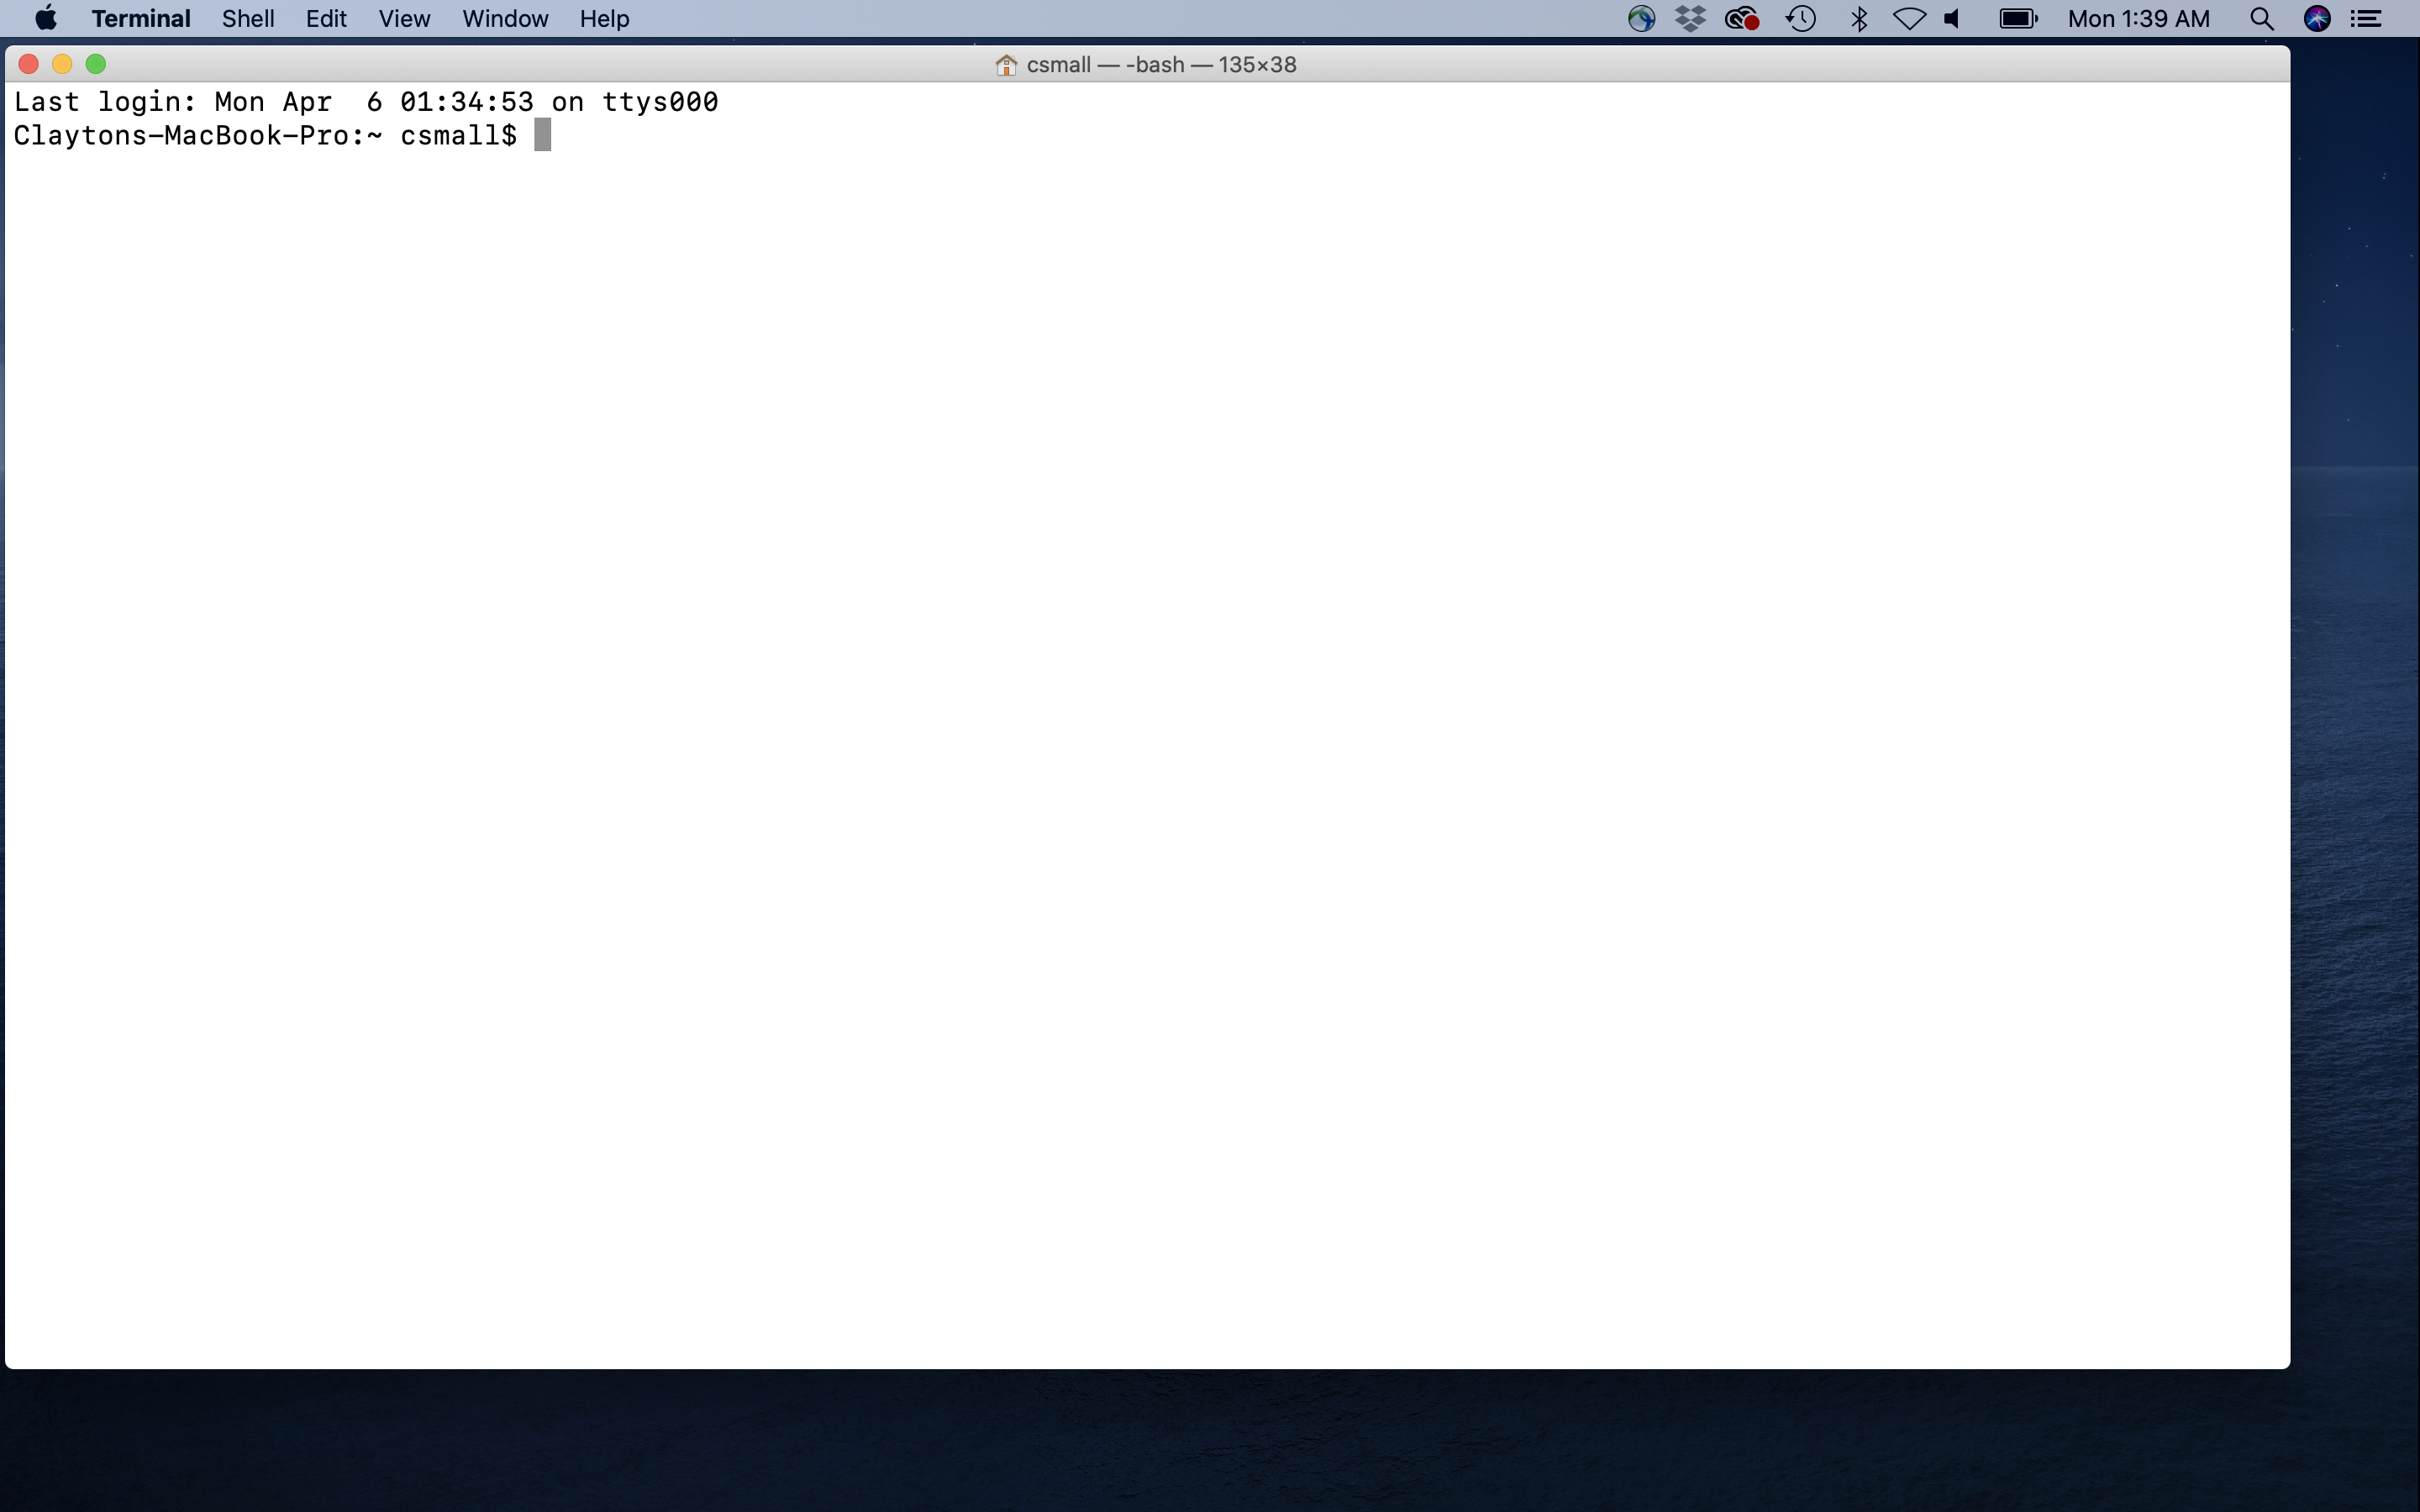
\includegraphics{/Users/csmall/github_repos/Found_Stat/images/MacTerminal.png}

You are now ready to navigate and explore files simply by typing!

\hypertarget{navigating-directories-and-files}{%
\subsection{Navigating directories and files}\label{navigating-directories-and-files}}

When you are at the command line, just think of your computer as you would if you were navigating using a graphical application (e.g.~Mac Finder or Windows Explorer). You are always in a directory in your file system, and you can move to any other directory by typing the approriate command and destination, then hitting Enter.

The first crucial UNIX command to learn is \texttt{pwd}. This command stands for ``print working directory,'' and it will literally print the path of the directory you are currently in.

Another important command is \texttt{ls}. This lists the files and directories (by default) in your working directory. If you specify a different directory, it will list the files and/or directories there. Most UNIX commands (and indeed command-line programs in general), can be run with options. One way to invoke the and option is to type a ``flag'' along with the command. In the case of \texttt{ls}, we can type \texttt{ls\ -l}, for example, which will print the output line-by-line. We can also add annother flag: \texttt{ls\ -lh} (equivalent to \texttt{ls\ -l\ -h}), which will print items line-by-line but also make sure the item sizes are ``human readable.'' If you ever have quesitons about how to use UNIX program, including the flags and other options, you can type \texttt{man\ program\_name} and a wonderful help manual will appear. To exit and return to the command prompt, just hit ``q''. These \texttt{man} pages are extremely useful and should be your first go-to if you need information for a particular command. Please use these regularly!

The command \texttt{cd} will change your location from the current directory to another directory. Like many other programs (UNIX and otherwise) require you to input directory and file locations, with \texttt{cd} you can specify your desired location using either the \emph{absolute} or \emph{relative} path. An absolute path is the full ``address'' of a directory or file, starting from the root of your file system. An example of an absolute path to a directory in my file system is \texttt{/Users/csmall/Dropbox/sculpin\_project/images/}. Regardless of where my current working directory is in my file system, I can change to this \texttt{images/} directory using \texttt{cd} and the full path. I can also use a relative path, which is a sort of ``shortcut,'' to specify the location of a directory or file. Let's say I am in \texttt{/Users/csmall/Dropbox/BiostatsFound\_S2020/} and I want to get to the \texttt{images/} directory above. I could type \texttt{cd\ ../sculpin\_project/images}, which uses a relative path to take me ``up'' one directory (as denoted by \texttt{../}) into \texttt{Dropbox/} and back ``down'' into \texttt{sculpin\_project/images}. In fact, \texttt{..} is a special file in every directory that just means ``the directory above.'' The special file \texttt{.} is the current directory. And to mention one final useful designation for navigation shortcuts, you can use the \texttt{\textasciitilde{}} to denote your home directory.

The schematic below should help you visualize how to think about file system navigation from the commmand line:
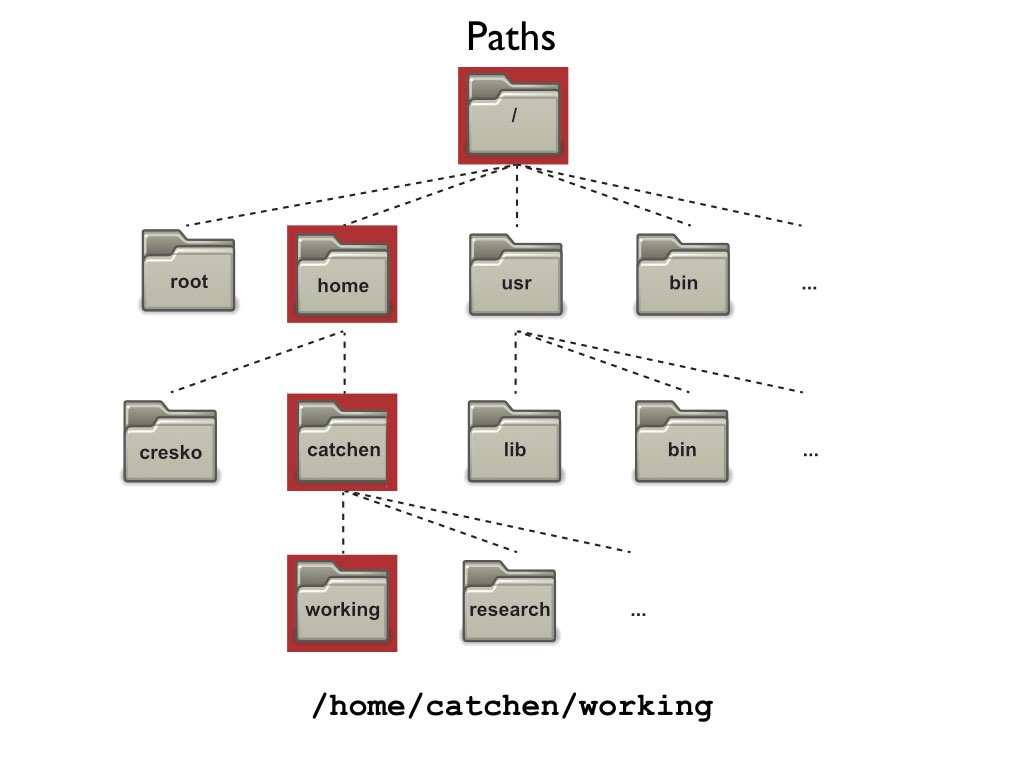
\includegraphics{/Users/csmall/github_repos/Found_Stat/images/Directory_example.jpeg}

And for another example, take a look at this series of navigation commands from my terminal and see if you can follow along:
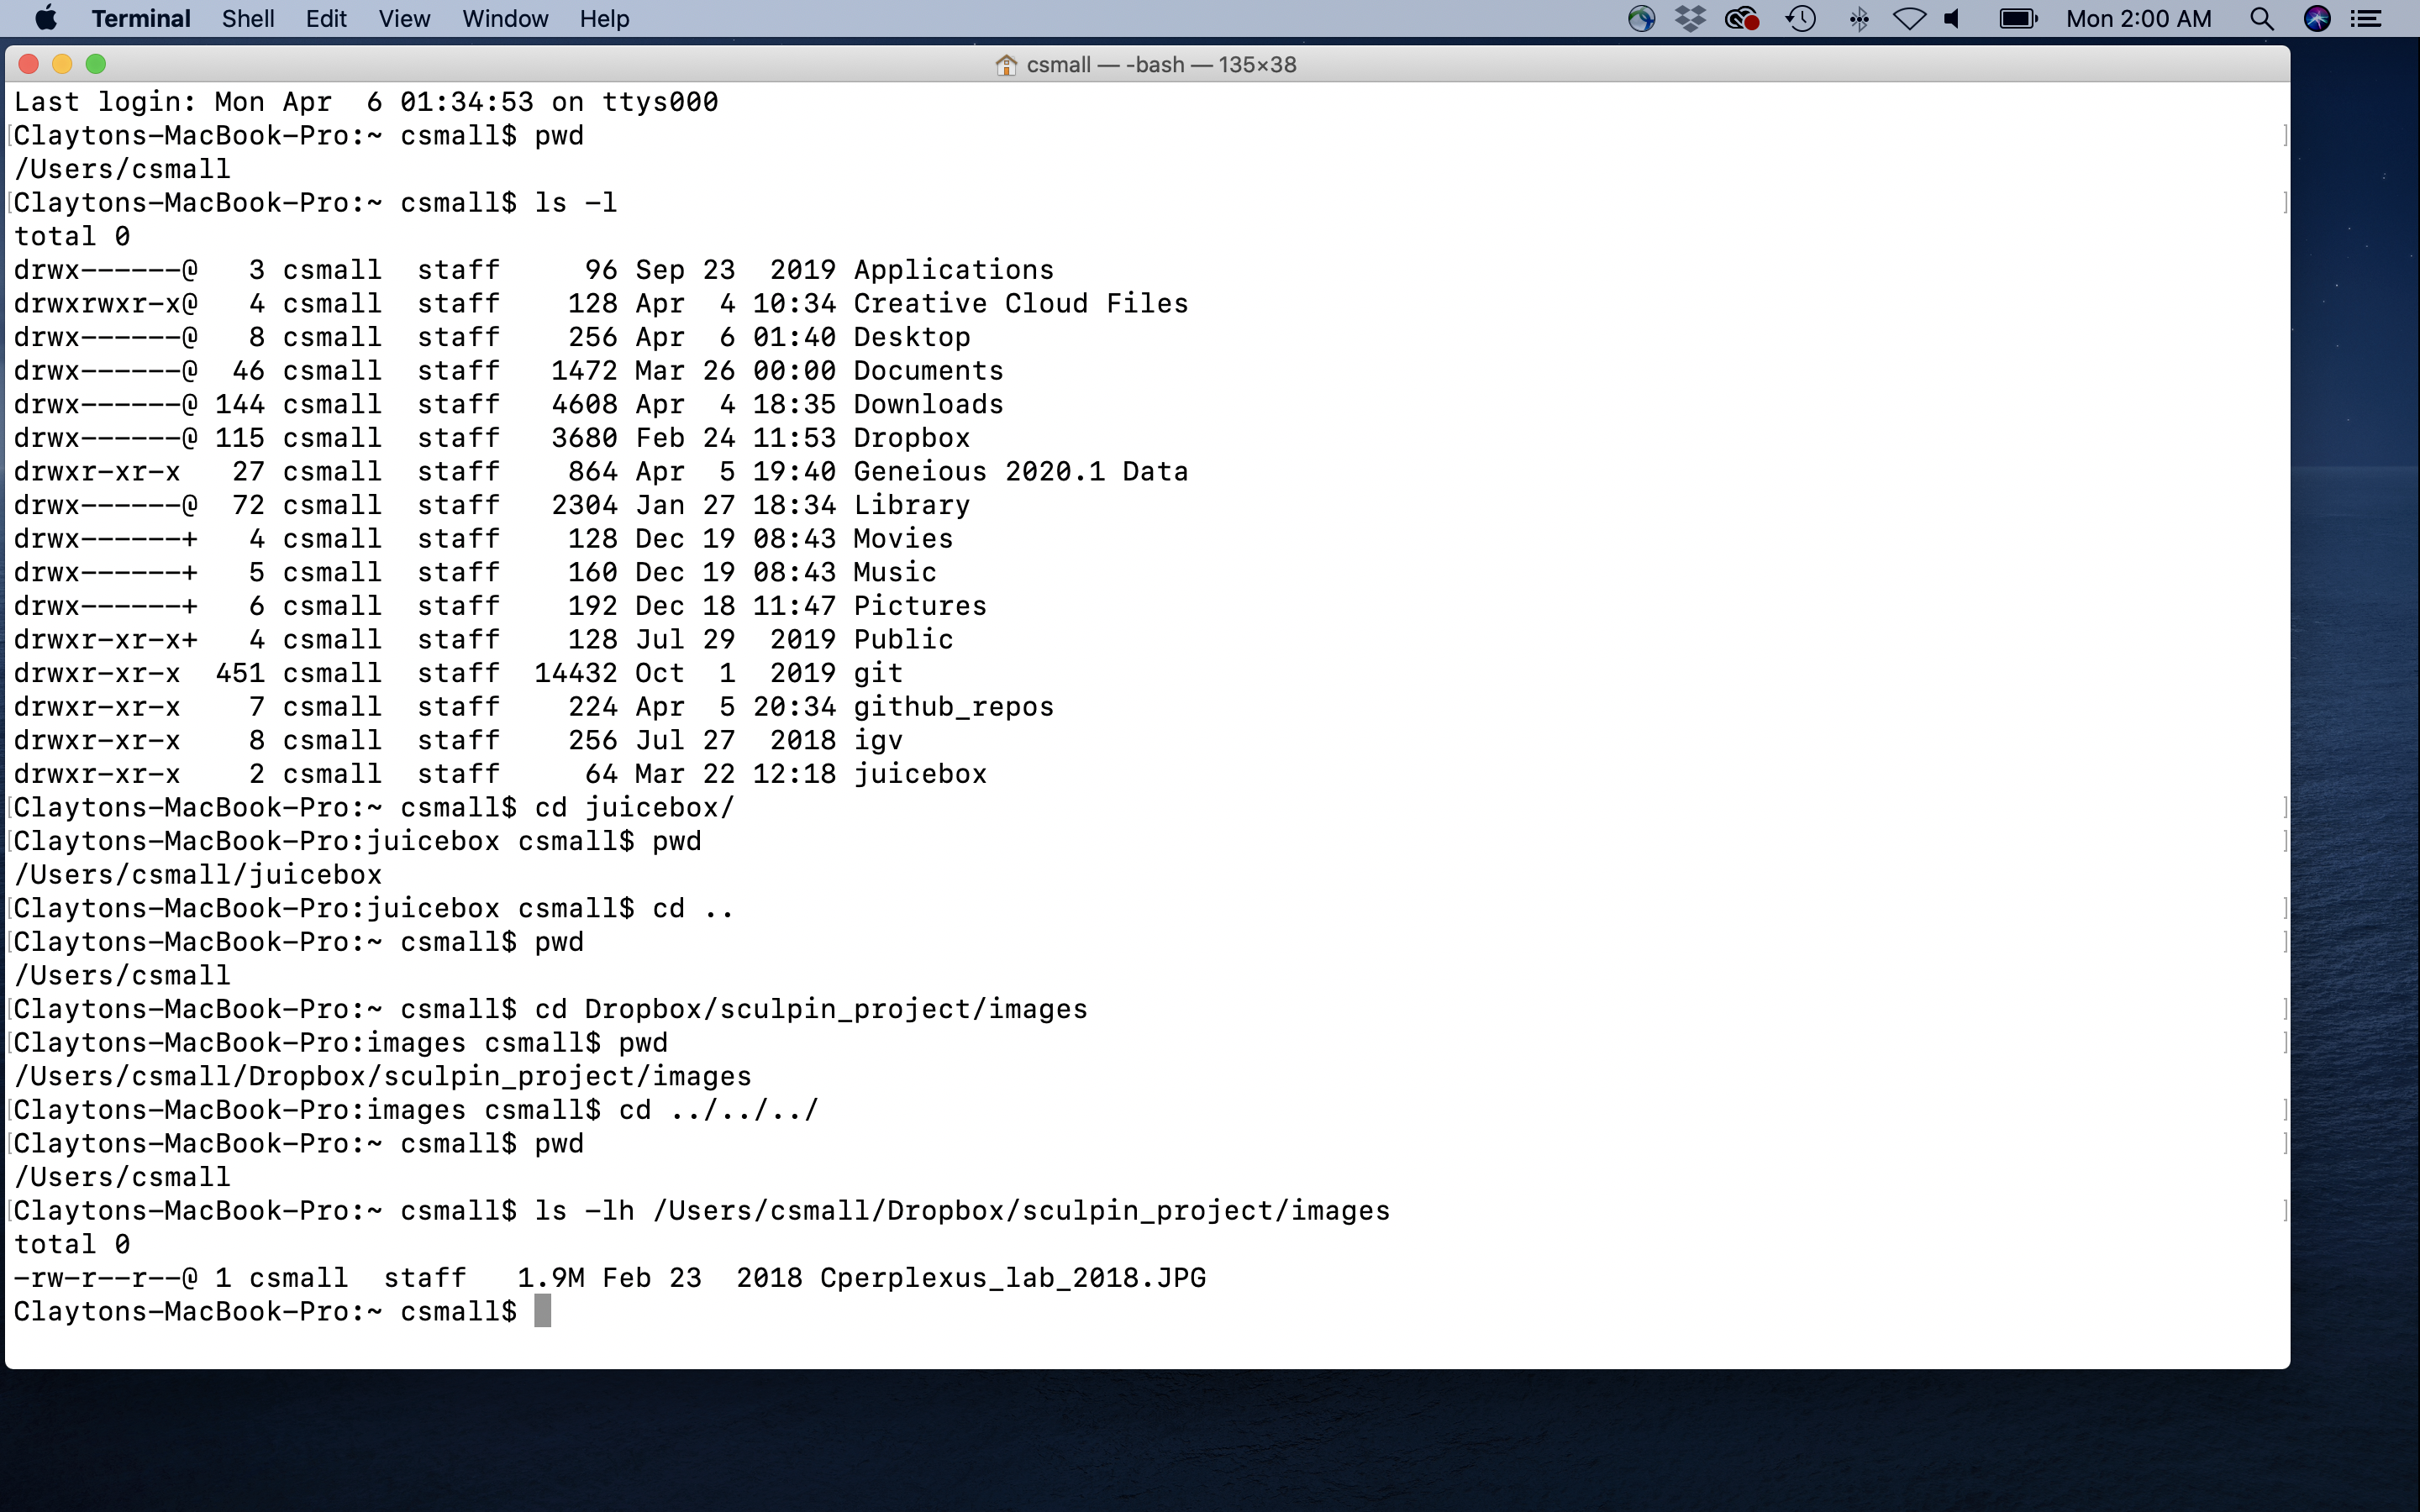
\includegraphics{/Users/csmall/github_repos/Found_Stat/images/MacTerminal_2.png}

If you want to create a new directory, you can use the \texttt{mkdir} command, including the desired name of the new directory. By default this will create the directory in your current working directory, but you can use absolute or relative paths to instead write the directory somewhere else. If you want to delete an empty directory, \texttt{rmdir} is the appropriate command.

Now let's briefly cover some UNIX commands that are useful for managing files. Some of these apply to directories as well, which I will point out as we go. The command \texttt{touch} can be used to create a new, empty file, which you can add to using a plain text editor. Examples of popular plain text editors with advanced user interfaces are BBEdit and Atom. You can also use command line text editors, such as \texttt{nano}, \texttt{emacs}, and \texttt{vim}. Most UNIX/LINUX systems have \texttt{nano} installed by default. To copy or change the name and/or location of a file (or directory), use \texttt{cp} and \texttt{mv} commands, respectively. Note that by using absolute or relative paths, you can specify where you want the file or directory to end up. Be especially careful with these, however, because you will overwrite any existing file or directory if you specify the same name and location. Another command you should be extremely cautious with is \texttt{rm}, which removes (permanently deletes) a file. \texttt{rm\ -r} can be used to delete a non-empty directory AND all of its contents.

In many cases you will want to look at files, or parts of them at least, from the command line. \texttt{cat} will print the entire contents of a file, but can also be used to combine (``concatenate'') multiple files in a line-wise manner. \texttt{less} and \texttt{more} will display specific lines of a file (starting with the first ones), with single- or multi-line ``scrolling,'' respectively, activated using the return or down-arrow keys. To leave the display, you need to hit the ``q'' key. \texttt{head} and \texttt{tail} will display the first or last, respectively, \emph{n} lines of the file, where \emph{n} is provided as a flag (e.g. \texttt{head\ -200\ file.tsv}). The ``word count'' command \texttt{wc} can quantify elements of a text file in various ways, but one common application is \texttt{wc\ -l}, which counts the number of lines in a file.

An aside: If you are working from the command line and want to terminate a process (say you accidentally start a task that will take way too long), press Ctrl-C.

\hypertarget{a-quick-review-of-important-unix-commands-for-navigation-and-viewing}{%
\subsubsection{A quick review of important UNIX commands for navigation and viewing}\label{a-quick-review-of-important-unix-commands-for-navigation-and-viewing}}

\texttt{pwd} - prints working directory

\texttt{ls} - lists contents of a directory

\texttt{cd} - changes the working directory

\texttt{mkdir} - creates a new directory

\texttt{rmdir} - deletes an empty directory

\texttt{touch} - creates an empty file

\texttt{cp} - copies a file or directory

\texttt{mv} - changes the name of a file or directory

\texttt{rm} - deletes a file, or a directory and everyting inside with \texttt{-r}

\texttt{cat} - prints the entire file to the terminal, or concatenates and prints multiple files

\texttt{less} - displays the first lines of a file, with scrolling line-by-line

\texttt{head} - prints the first 10 lines (default) of a file

\texttt{tail} - prints the last 10 lines (default) of a file

\texttt{wc\ -l} - prints the number of lines in a file

\hypertarget{useful-unix-commands-for-file-manipulation}{%
\subsection{Useful UNIX commands for file manipulation}\label{useful-unix-commands-for-file-manipulation}}

In many cases you will want to search for specific characters or combinations of characters, and do various things with that information. Maybe you want to isolate the lines of a file that contain the query, or perhaps you want to count how many lines contain the query. The tool \texttt{grep} is extremely useful in this regard. We don't have time for a comprehensive dive into the utilities of \texttt{grep}, but a few common applications are worth mentioning. Character patterns we search for using \texttt{grep} may or may not involve special characters that are not interpretted literally. Here we will discuss just a few common cases of \texttt{grep} searches and the special characters involved. Some examples of these special characters include \texttt{\^{}} (beginning of a line), \texttt{\$} (end of a line), \texttt{.} (any single character except a newline), \texttt{*} (zero or more instances of the preceeding character), and \texttt{\textbackslash{}s} (any white space). The standard syntax for \texttt{grep} from the command line is \texttt{grep\ "expression"\ filename}. So, if you wanted to return all of the lines in the data file \texttt{zfish\_data.tsv} (assuming it is in the current directory) that begin with ``embryo\_10'', you could try \texttt{grep\ "\^{}embryo\_10"\ zfish\_data.tsv}. This search would also (unintentionally) find lines beginning with ``embryo\_100'' or ``embryo\_101'', etc., if they exist. So, you have to be careful, and learning the rules just takes practice. In this case \texttt{grep\ "\^{}embryo\_10\textbackslash{}s"\ zfish\_data.tsv} would acheive the desired result, assuming that there is a whitespace delimiter between fields (``columns'') in the data file. Useful flags for \texttt{grep} include \texttt{-c} (which counts the number of lines containing the query), \texttt{-v} (which returns the lines that \emph{do not} contain the query), and \texttt{-n} (which prints the line number for each line containing the query). I encourage you to look at many different \texttt{grep} use cases online as your demand for complex searches grows.

The program \texttt{sed} has reasonably complex applciations, but is commonly used as a sort of ``search and replace'' tool. The syntax for \texttt{sed} use is similar to \texttt{grep}, except that the query and replacement expressions are organized (with other information) using slashes. For ``search and replace'' functionality, that sytax looks like this: \texttt{sed\ \textquotesingle{}s/query/replacement/flag\textquotesingle{}\ filename}. One common option for the ``flag'' component is ``g'', meaning ``global'', which replaces all instances. If no flag designation is made only the first instance in the file is replaced. Building on our toy example from above, \texttt{sed\ \textquotesingle{}s/\^{}embryo\_/\^{}larva\_/g\textquotesingle{}\ zfish\_data.tsv} would perform a global replacement and print the output to the terminal. To change the contents in the original file on the fly, including \texttt{sed\ -i} would do the trick, but is riskier than redirecting the output to a new file.

\texttt{cut} is quite straightforward, and can be used to isolate individual fields (think of them like ``columns'') from a text file, provided the fields are consistently separated by a delimeter on each line. So, if I had a comma-separated file and I just wanted the first two columns I could type \texttt{cut\ -f1,2\ -d"\textbackslash{}t"\ filename}. Note that if you don't specify a delimter using the \texttt{-d} flag, then it is assumed to be tab-delimited. If you want to bring together fields in separate files, \texttt{join} can be used to accomplish this. The two files should have equivalent rows, however, for this action to work properly.

If you want to sort text files alphanumerically, in a field-wise fashion, \texttt{sort} is quite useful. If a file contains a single field, minimal specification is required, aside from tuning numerical sorting. For example, if you want to sort numerically, use the \texttt{-n} flag, and if you want to sort from largest to smallest, add the \texttt{-r} flag. If you want to sort a multi-field file based on just one field, you can use the ``key'' flag. For instance, if you have a tab-delimited file and want to sort by the second field in reverse numerical order, \texttt{sort\ -k2,2\ -nr\ filename.tsv} would give you the desired result. Finally, if you want to eliminate lines with the same value for a given field, you can use the \texttt{-u} ``unique'' flag.

The UNIX program \texttt{awk} is an extremely powerful tool, and can itself be used essentially as a mini programming language. We will not get into the myriad uses of \texttt{awk} here, but the reference at the bottom of the chapter is a great resource if you want to learn more. \texttt{awk} is extremely efficient at parsing and capturing text files in a column-wise manner, with the ability to also evaluate logical statements applied to rows. The structure of \texttt{awk} commands is more complex than that of other UNIX programs we have discussed, but it is still very intuitive. One unique feature is that \texttt{awk} contains its own internal functions, which are typed inside curly braces. The ``print'' function can be used to extract fields, much like \texttt{cut}. For instance, \texttt{awk\ -F:\ \textquotesingle{}\{print\ \$1,\$6\}\textquotesingle{}\ filename.tsv} would print the first and sixth field from \texttt{filename.tsv}, assuming a ``:'' delimiter. With \texttt{awk}, fields are specified using the \texttt{\$} character. If you want also to select only specific rows from a set of columns (like those with a certain value), you can incorporate logical operators. In the above example if we had wanted fields 1 and 6, but only those rows with a value of at least 610 in field 4, we could type the following \texttt{awk\ -F:\ \textquotesingle{}\$4\ \textgreater{}=\ 610\ \{print\ \$1,\$6\}\textquotesingle{}\ filename.tsv}. Again, this is just scratching the surface with \texttt{awk}, which boasts a great deal of potential for your text file manipulation needs.

\hypertarget{a-quick-review-of-key-unix-commands-for-text-file-searching-and-manipulation}{%
\subsubsection{A quick review of key UNIX commands for text file searching and manipulation}\label{a-quick-review-of-key-unix-commands-for-text-file-searching-and-manipulation}}

\texttt{grep} - searches a file for characters and character combinations

\texttt{sed} - stream edits characters and character combinations

\texttt{cut} - isolates specific fields (``columns'') from a file using a delimiter

\texttt{join} - combines fields (``columns'') from multiple files with equivalent rows

\texttt{sort} - orders the rows in a file based on one or more fields

\texttt{awk} - flexibly parses, evaluates, and selectively prints row- and column-wise

\hypertarget{a-quick-word-on-pipes-and-carrots}{%
\subsection{A quick word on pipes and carrots}\label{a-quick-word-on-pipes-and-carrots}}

One very convenient feature of UNIX commands is that you can control the flow of input and output from one command to another using the \texttt{\textbar{}} (``pipe'') character. For instance, I may want to search an entire file for rows that begin with ``fish-1'', and then replace the ``-'' with "\_``. To do this I could do something like \texttt{cat\ file.tsv\ \textbar{}\ grep\ "\^{}fish-1"\ \textbar{}\ sed\ \textquotesingle{}s/fish-1/fish\_1/g\textquotesingle{}} This, of course, would print the output to the terminal, but I could actually capture that output into a file using the \texttt{\textgreater{}} charcter. \texttt{cat\ filename\ \textbar{}\ grep\ "\^{}fish-1"\ \textbar{}\ sed\ \textquotesingle{}s/fish-1/fish\_1/g\textquotesingle{}\ \textgreater{}\ ./newfile.tsv} would write this new file to my current working directory. Furthermore, if you want to append lines of text to an existing file, the''double sideways right-pointing carrot" character \texttt{\textgreater{}\textgreater{}} can be used.

The above lessons on UNIX commands for file manipulation truly just scratch the surface of what can be accomplished at the command line and in ``shell scripts.'' You certainly will have further questions and be hungry for more, but we simply don't have time during this course. But to work on your UNIX skills for now, check out \texttt{Ex1\_Unix\_Intro.html} (on Canvas). We need to move on to R now, but at the bottom of this chapter are some UNIX command resources I have found to be especially useful.

\hypertarget{data-file-and-data-file-entry-dos-and-donts}{%
\section{Data file and data file entry dos and don'ts}\label{data-file-and-data-file-entry-dos-and-donts}}

Do store a copy of your data in a nonproprietary format, such as plain ASCII text (aka a flat file). This is especially important if you are using tools (like UNIX commands) to parse and manipulate the files. Formats like Microsoft Excel are not acceptable as input for many analysis tools, and not everyone has access to proprietary software.

Do leave an un-edited copy of an original data file, even when main analyes require an edited version.

Do use descriptive names for your data files and variables, and use them consistently!

Do maintain effective metadata about the data.

Do add new observations to a data file as rows.

Do add new variables to a data file as columns.

Don't include multiple data types in the same column.

Don't use non-alphanumeric characters (other than the underscore) in file or directory names.

Don't use spaces, tabs, commas, colons, semicolons, or other chacters commonly used as field (column) delimiters in names of individual data entries. For example, don't use something like \texttt{March\ 8} as a value for date in a data set.

Don't copy and paste data directly from rich-text-formatted files (like Microsoft Word) into primary data files.

\hypertarget{exercises-associated-with-this-chapter}{%
\section{Exercises associated with this chapter:}\label{exercises-associated-with-this-chapter}}

\begin{itemize}
\tightlist
\item
  Exercise 1 (file: \texttt{Ex1\_Unix\_Intro.html})
\end{itemize}

\hypertarget{additional-learning-resources}{%
\section{Additional learning resources}\label{additional-learning-resources}}

\begin{itemize}
\item
  \url{http://mally.stanford.edu/~sr/computing/basic-unix.html} - A nice ``cheat sheet''
\item
  \url{http://korflab.ucdavis.edu/Unix_and_Perl/} - Outstanding tutorial by Keith Bradnam and Ian Korf
\item
  \url{https://www.datacamp.com/courses/introduction-to-shell-for-data-science} - DataCamp tutorial
\item
  \url{https://www.gnu.org/software/gawk/manual/gawk.html} - A comprehensive guide to \texttt{awk}
\end{itemize}

\hypertarget{an-introduction-to-the-r-language}{%
\chapter{An Introduction to the R language}\label{an-introduction-to-the-r-language}}

\hypertarget{background}{%
\section{Background}\label{background}}

\texttt{R} is a computer programming language and environment especially useful for graphic visualization and statistical analysis of data. It is an offshoot of a language developed in 1976 at Bell Laboratories called \texttt{S}. \texttt{R} is an interpreted language, meaning that every time code is run it must be translated to machine language by the \texttt{R} interpreter, as opposed to being compiled prior to running. \texttt{R} is the premier computational platform for statistical analysis thanks to its GNU open-source status and countless packages contributed by diverse members of the scientific community.

\hypertarget{why-use-r}{%
\section{\texorpdfstring{Why use \texttt{R}?}{Why use R?}}\label{why-use-r}}

\begin{itemize}
\tightlist
\item
  Good general scripting tool for statistics and mathematics
\item
  Powerful and flexible and free
\item
  Runs on all computer platforms
\item
  New packages released all the time
\item
  Superb data management \& graphics capabilities
\item
  Reproducibility - can keep your scripts to see exactly what was done
\item
  Can embed your \texttt{R} analyses in dynamic, polished files using R markdown
\item
  You can write your own functions
\item
  Lots of online help available
\item
  Can use a nice IDE such as \texttt{RStudio}
\end{itemize}

\hypertarget{important-r-terms-and-definitions}{%
\section{\texorpdfstring{Important \texttt{R} terms and definitions}{Important R terms and definitions}}\label{important-r-terms-and-definitions}}

\begin{figure}
\centering
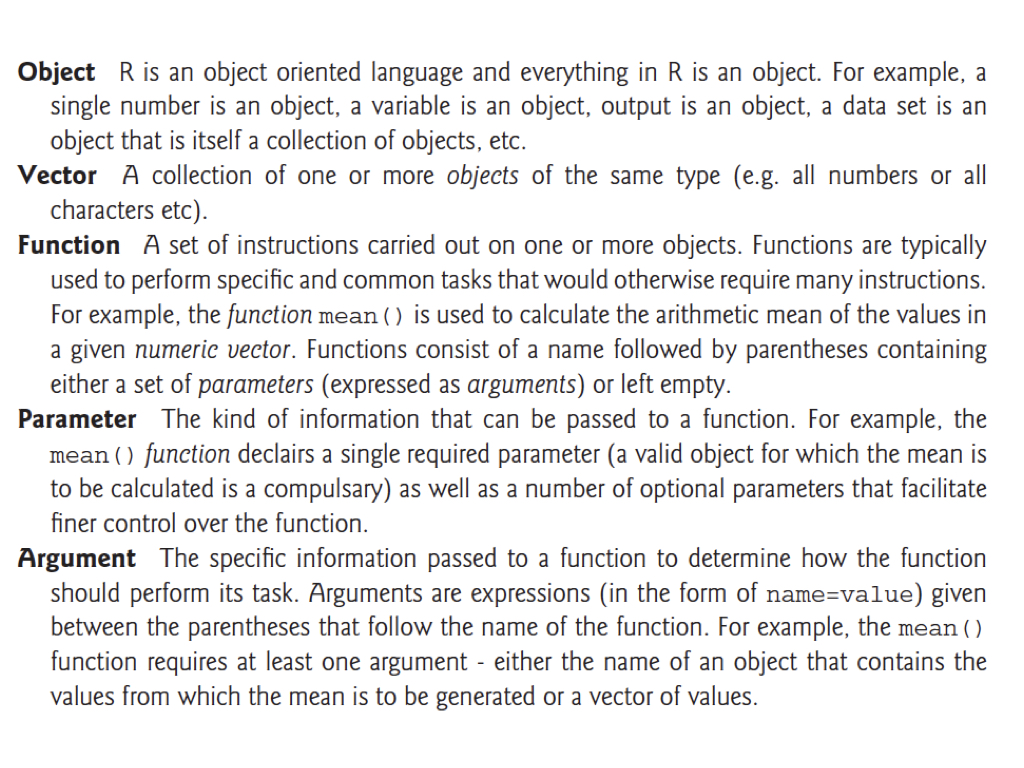
\includegraphics{/Users/csmall/github_repos/Found_Stat/images/R_definitions_Logan.001.jpeg}
\caption{Alt text}
\end{figure}

From Logan, M. 2010. \emph{Biostatistical Design and Analysis Using R}

Operators are symbols in programming that have a specific meaning

\begin{figure}
\centering
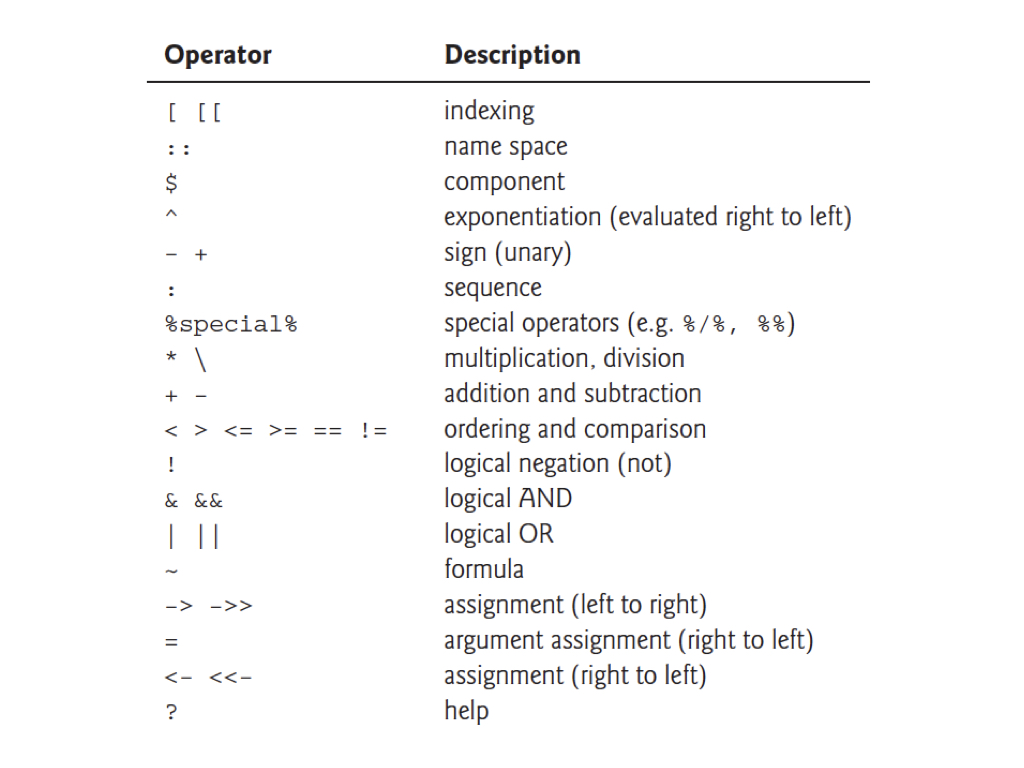
\includegraphics{/Users/csmall/github_repos/Found_Stat/images/R_definitions_Logan.002.jpeg}
\caption{Alt text}
\end{figure}

From Logan, M. 2010. \emph{Biostatistical Design and Analysis Using R}

\hypertarget{getting-started-with-r-via-the-rstudio-environment}{%
\section{\texorpdfstring{Getting started with \texttt{R} via the RStudio Environment}{Getting started with R via the RStudio Environment}}\label{getting-started-with-r-via-the-rstudio-environment}}

To begin working with \texttt{R}, open RStudio. You should first see something that looks like this:
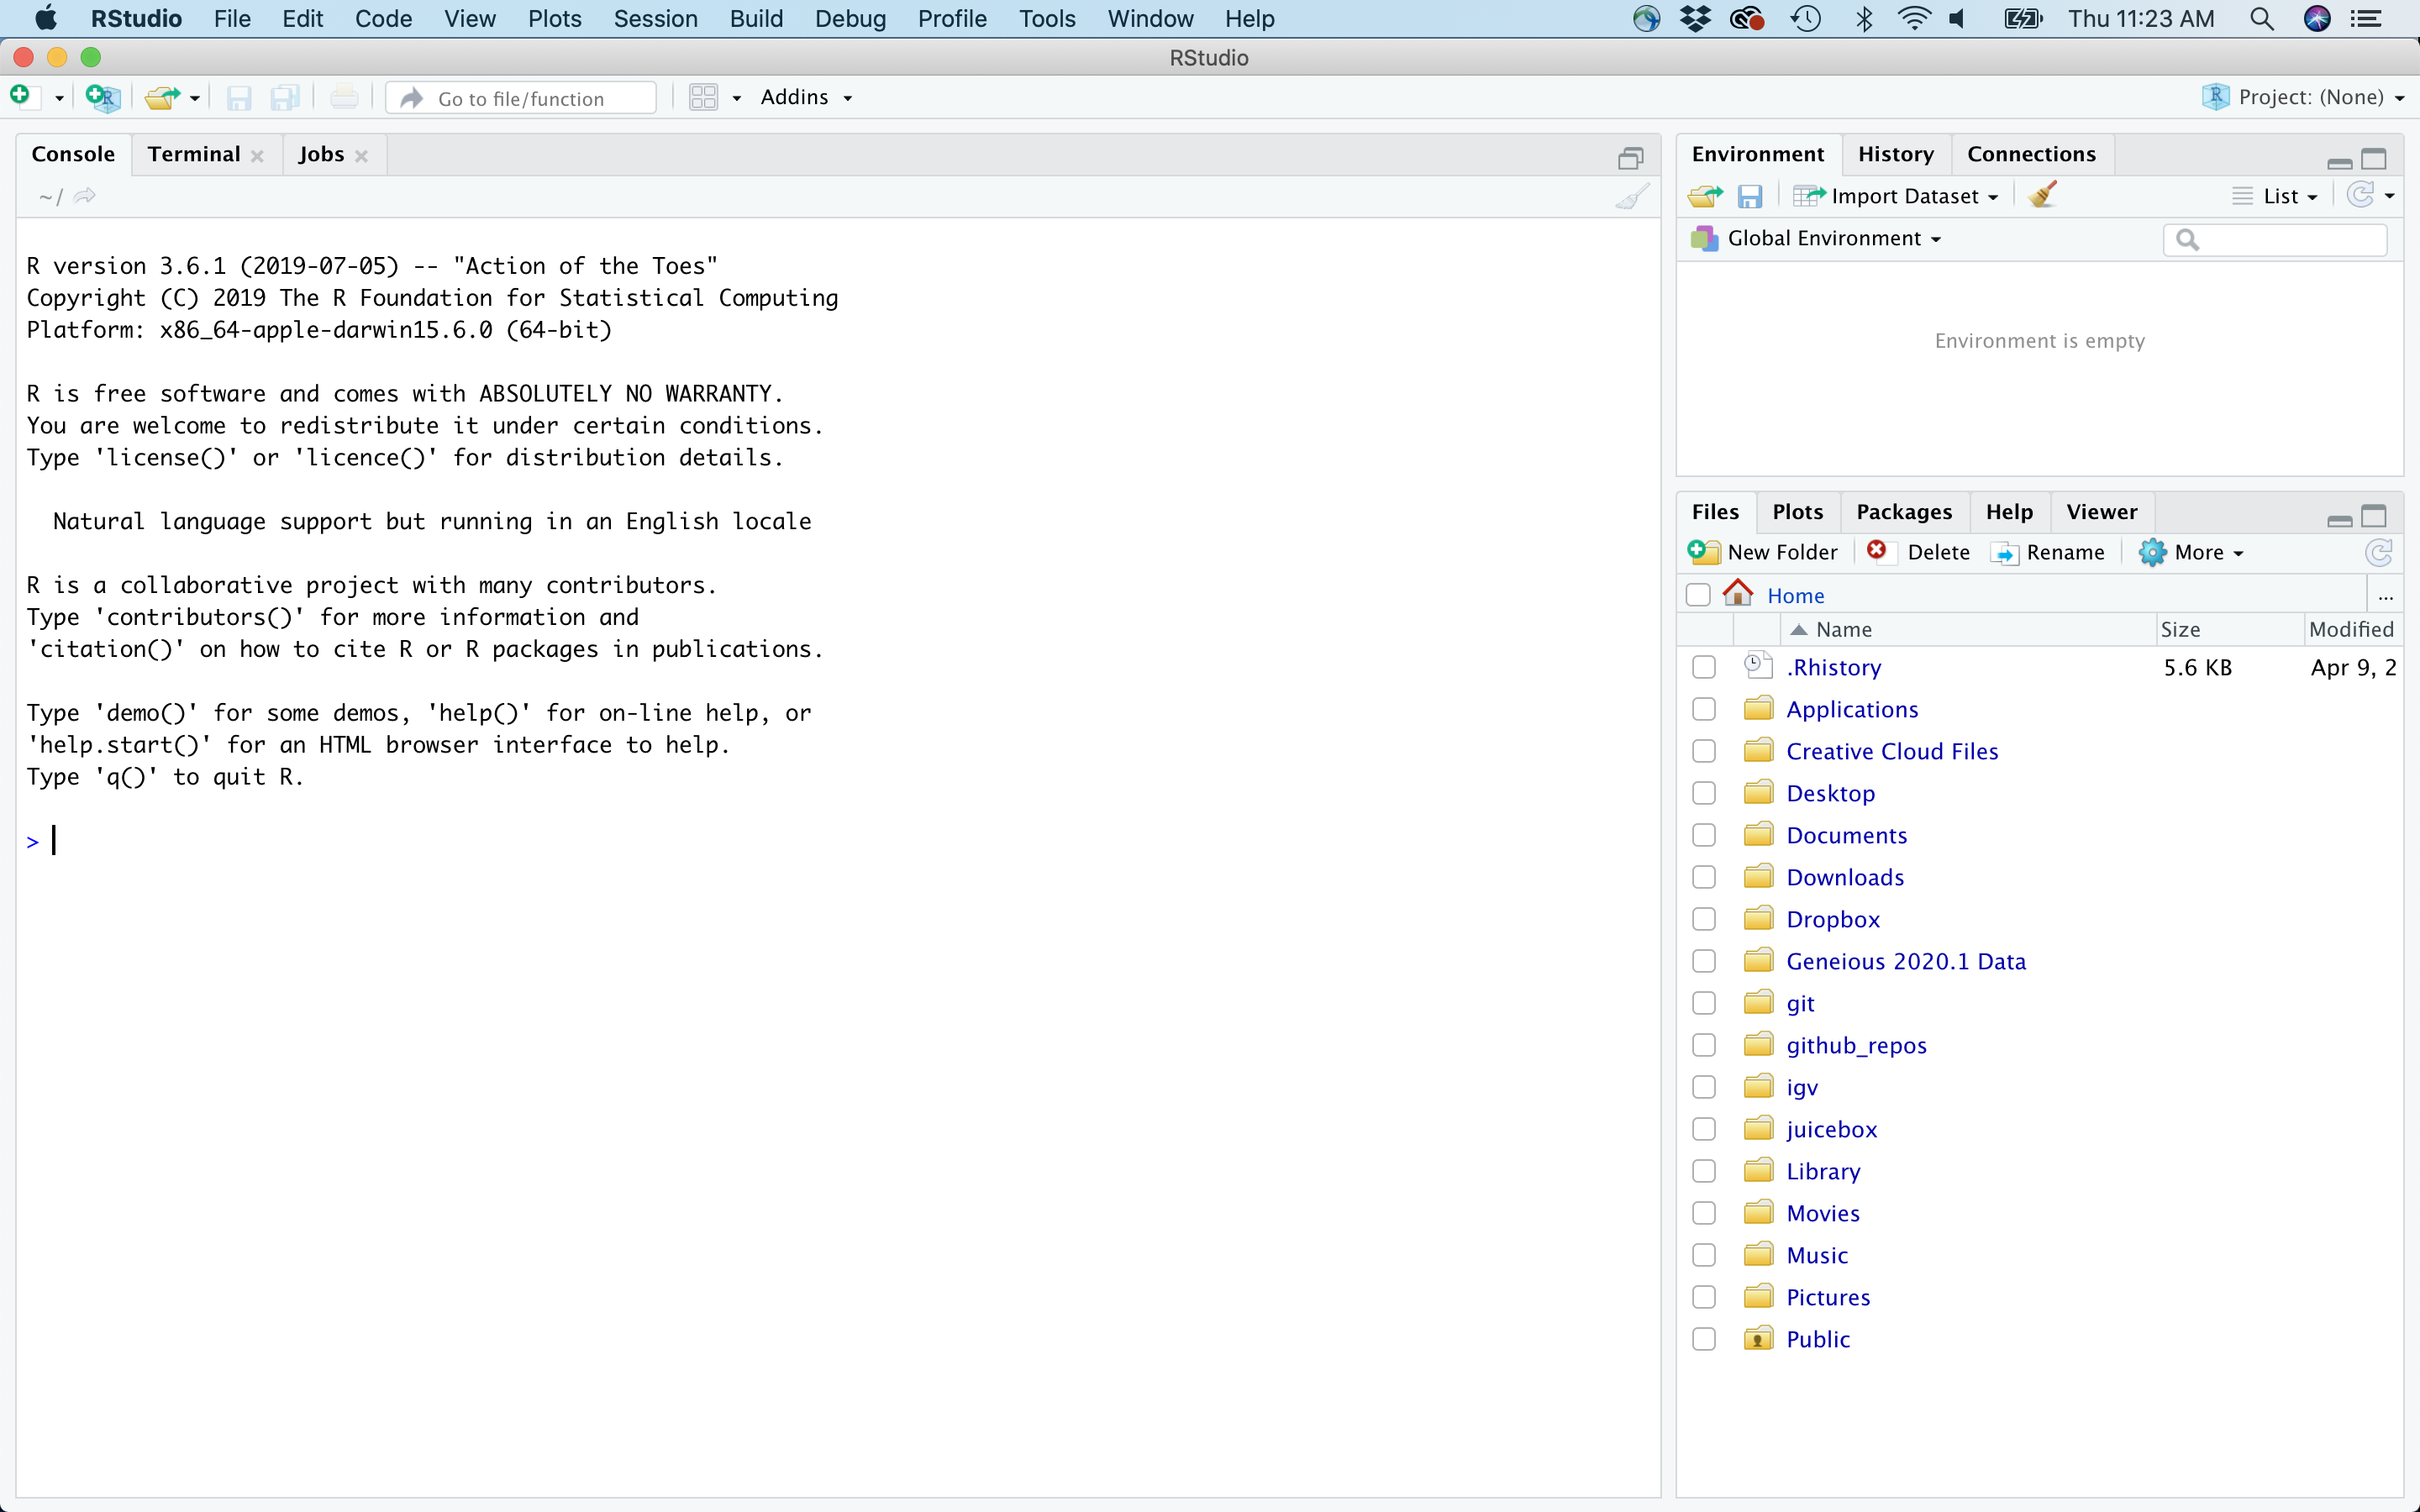
\includegraphics{/Users/csmall/github_repos/Found_Stat/images/MacTerminal_3.png}

To open a new script editor (where you will keep track of your code and notes), go to File \textgreater{} New File \textgreater{} R Script. Note that there are other options for file types, which we will be using in the future. For now, though, we want a plain script, which when saved will have the extention \texttt{.R}.

It is easy to run code directly from the script editor. For single lines of code, simply make sure your cursor is on that line, and hit Ctrl-Enter. For multiple lines, highlight the block of code you want to run and hit Ctrl-Enter.

Now your display should look somehting like below (but without the red pane labels, of course):
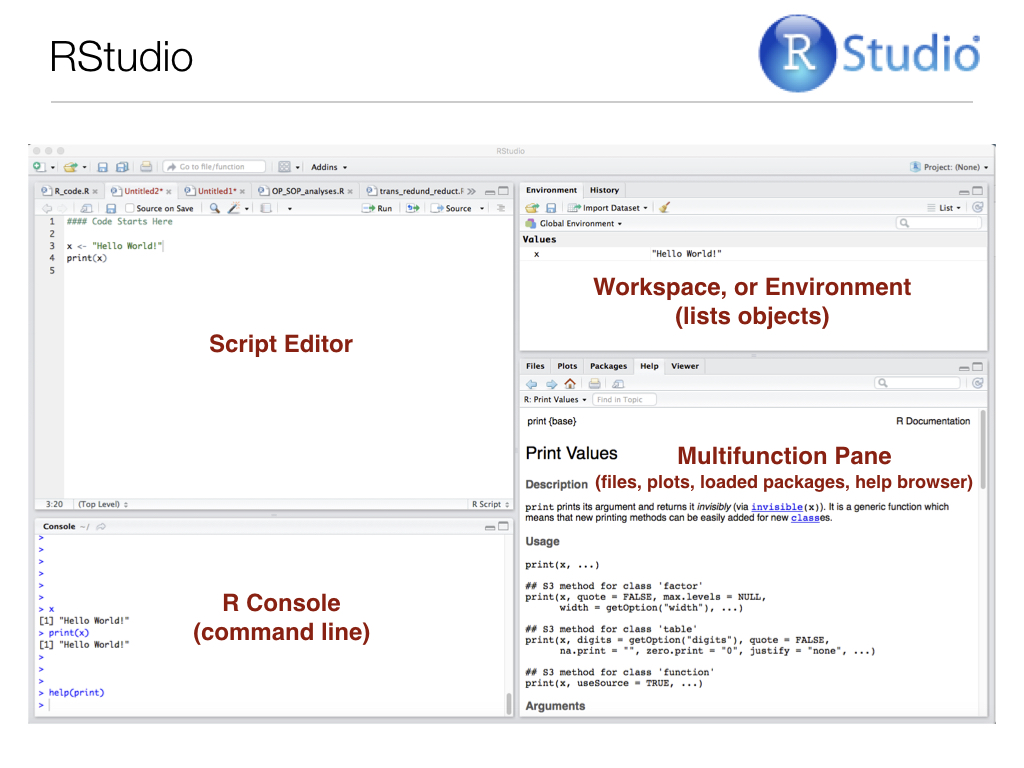
\includegraphics{/Users/csmall/github_repos/Found_Stat/images/R_definitions_Logan.003.jpeg}

Note that you can also type commands directly from the command line using the \texttt{R} Console (lower left pane), and the \texttt{R} interpreter will run them when you press Enter.

Any objects you define, and a summary of their values, will appear in the upper right pane, and the lower right pane differs in appearance depending on instructions you provide to \texttt{R\ Studio}. For instance, if you produce a plot, it will appear there by default. Another extremely important feature of R functions (we'll get to them in a bit) is the help file. Recall from Chapter 5 our discussion of \texttt{man} pages for UNIX programs. Help files the equivalent for \texttt{R} functions. They contain almost everything you need to know about a given function, and most of them even include and example at the bottom. These help files will appear in the lower right RStudio pane when you call them, for example when you run \texttt{help(function\_name)} at the \texttt{R} Console.

\hypertarget{r-programming-basics}{%
\subsection{R Programming Basics}\label{r-programming-basics}}

For the code examples below, it might be useful for you to start your own RStudio session, open a new \texttt{.R} file and type/run code while reading.

\begin{itemize}
\tightlist
\item
  Commands can be submitted through the terminal, console or scripts
\item
  In your scripts, anything that follows \texttt{\#} symbol (aka hash) is just for humans
\item
  Notice on these slides I'm evaluating the code chunks and showing output
\item
  The output is shown here after the two \texttt{\#} symbols and the number of output items is in \texttt{{[}{]}}
\item
  Also notice that \texttt{R} follows the normal priority of mathematical evaluation
\end{itemize}

\begin{Shaded}
\begin{Highlighting}[]
\DecValTok{4}\OperatorTok{*}\DecValTok{4}
\end{Highlighting}
\end{Shaded}

\begin{verbatim}
## [1] 16
\end{verbatim}

\begin{Shaded}
\begin{Highlighting}[]
\NormalTok{(}\DecValTok{4}\OperatorTok{+}\DecValTok{3}\OperatorTok{*}\DecValTok{2}\OperatorTok{^}\DecValTok{2}\NormalTok{)}
\end{Highlighting}
\end{Shaded}

\begin{verbatim}
## [1] 16
\end{verbatim}

\hypertarget{a-note-on-r-markdown}{%
\subsubsection{\texorpdfstring{A note on \texttt{R} Markdown}{A note on R Markdown}}\label{a-note-on-r-markdown}}

This format provides a much better way to embed code and output, in an easily readable, reproducible manner. We will dive into \texttt{R} Markdown next week, so for now just be aware that it exists.

\begin{itemize}
\item
  \url{http://kbroman.org/knitr_knutshell/pages/Rmarkdown.html}
\item
  You can insert \texttt{R} chunks into \texttt{Rmarkdown} documents
\end{itemize}

\hypertarget{assigning-variables}{%
\subsubsection{Assigning Variables}\label{assigning-variables}}

\begin{itemize}
\item
  To ``store'' information for later use, like the arithmetic operation above, we can assign variables in \texttt{R}.
\item
  Variables are assigned values using the \texttt{\textless{}-} operator.
\item
  Variable names must begin with a letter, and should not contain spaces or \texttt{R} operators (see above) but other than that, just about anything goes.
\item
  Do keep in mind that \texttt{R} is case sensitive.
\end{itemize}

\begin{Shaded}
\begin{Highlighting}[]
\NormalTok{x <-}\StringTok{ }\DecValTok{2}
\NormalTok{x }\OperatorTok{*}\StringTok{ }\DecValTok{3}
\end{Highlighting}
\end{Shaded}

\begin{verbatim}
## [1] 6
\end{verbatim}

\begin{Shaded}
\begin{Highlighting}[]
\NormalTok{y <-}\StringTok{ }\NormalTok{x }\OperatorTok{*}\StringTok{ }\DecValTok{3}
\NormalTok{y }\OperatorTok{-}\StringTok{ }\DecValTok{2}
\end{Highlighting}
\end{Shaded}

\begin{verbatim}
## [1] 4
\end{verbatim}

These do not work

\begin{Shaded}
\begin{Highlighting}[]
\NormalTok{3y <-}\StringTok{ }\DecValTok{3}
\DecValTok{3}\OperatorTok{*}\NormalTok{y <-}\StringTok{ }\DecValTok{3}
\end{Highlighting}
\end{Shaded}

\hypertarget{arithmetic-operations-with-functions}{%
\subsubsection{Arithmetic operations with functions}\label{arithmetic-operations-with-functions}}

\begin{itemize}
\item
  Arithmetic operations can be used with functions as well as numbers.
\item
  Try the following, and then your own.
\end{itemize}

\begin{Shaded}
\begin{Highlighting}[]
\NormalTok{x}\OperatorTok{+}\DecValTok{2}
\NormalTok{x}\OperatorTok{^}\DecValTok{2}
\KeywordTok{log}\NormalTok{(x) }\OperatorTok{+}\StringTok{ }\KeywordTok{log}\NormalTok{(x}\OperatorTok{+}\DecValTok{1}\NormalTok{)}
\end{Highlighting}
\end{Shaded}

\begin{itemize}
\item
  Note that the last of these - \texttt{log()} - is a built in function of \texttt{R}, and therefore the argument for the function (in this case ``x'' or ``x+1'') needs to be put in parentheses.
\item
  These parentheses will be important, and we'll come back to them later when we add other arguments after the object in the parentheses.
\item
  The outcome of calculations can be assigned to new variables as well, and the results can be checked using the \texttt{print()} function.
\end{itemize}

\begin{Shaded}
\begin{Highlighting}[]
\NormalTok{y <-}\StringTok{ }\DecValTok{67}
\KeywordTok{print}\NormalTok{(y)}
\end{Highlighting}
\end{Shaded}

\begin{verbatim}
## [1] 67
\end{verbatim}

\begin{Shaded}
\begin{Highlighting}[]
\NormalTok{x <-}\StringTok{ }\DecValTok{124}
\NormalTok{z <-}\StringTok{ }\NormalTok{(x}\OperatorTok{*}\NormalTok{y)}\OperatorTok{^}\DecValTok{2}
\KeywordTok{print}\NormalTok{(z)}
\end{Highlighting}
\end{Shaded}

\begin{verbatim}
## [1] 69022864
\end{verbatim}

\hypertarget{strings}{%
\subsubsection{Strings}\label{strings}}

\begin{itemize}
\item
  Assignments and operations can be performed on characters as well.
\item
  Note that characters need to be set off by quotation marks to differentiate them from numeric objects.
\item
  The c(function) stands for `concatenate'.
\item
  Note that we are using the same variable names as we did previously, which means that we're overwriting our previous assignment.
\item
  A good general rule is to use new names for each variable, and make them short but still descriptive
\end{itemize}

\begin{Shaded}
\begin{Highlighting}[]
\NormalTok{x <-}\StringTok{ "I Love"}
\KeywordTok{print}\NormalTok{ (x)}
\end{Highlighting}
\end{Shaded}

\begin{verbatim}
## [1] "I Love"
\end{verbatim}

\begin{Shaded}
\begin{Highlighting}[]
\NormalTok{y <-}\StringTok{ "Biostatistics"}
\KeywordTok{print}\NormalTok{ (y)}
\end{Highlighting}
\end{Shaded}

\begin{verbatim}
## [1] "Biostatistics"
\end{verbatim}

\begin{Shaded}
\begin{Highlighting}[]
\NormalTok{z <-}\StringTok{ }\KeywordTok{c}\NormalTok{(x,y)}
\KeywordTok{print}\NormalTok{ (z)}
\end{Highlighting}
\end{Shaded}

\begin{verbatim}
## [1] "I Love"        "Biostatistics"
\end{verbatim}

The variable z is now a vector of character objects.

\hypertarget{factors}{%
\subsubsection{Factors}\label{factors}}

\begin{itemize}
\item
  Sometimes we would like to treat character objects as if they were units for subsequent calculations.
\item
  These are called factors, and we can redefine our character object as one of class factor.
\item
  This might seem a bit strange, but it's important for statistical analyses where we might want to calculate the mean or variance for two different treatments. In that case the two different treatments would be coded as two different ``levels'' of a factor we designate in our metadata. This will become clear when we get into hypothesis testing in \texttt{R}.
\end{itemize}

\begin{Shaded}
\begin{Highlighting}[]
\NormalTok{z_factor <-}\StringTok{ }\KeywordTok{as.factor}\NormalTok{(z)}
\KeywordTok{print}\NormalTok{(z_factor)}
\KeywordTok{class}\NormalTok{(z_factor)}
\end{Highlighting}
\end{Shaded}

Note that factor levels are reported alphabetically. I used the \texttt{class()} function to ask \texttt{R} what type of object ``z\_factor'' is. \texttt{class()} is one of the most important tools at your disposal. Often times you can debug your code simply by changing the class of an object. Because functions are written to work with specific classes, changing the class of a given object is crucial in many cases.

\hypertarget{vectors}{%
\subsubsection{Vectors}\label{vectors}}

\begin{itemize}
\item
  In general R thinks in terms of vectors (a list of characters factors or numerical values) and it will benefit any R user to try to write programs with that in mind.
\item
  R operations, and therefore functions, are vectorized.
\item
  This means an operation or function will be performed for each element in a vector.
\item
  Vectors can be assigned directly using the `c()' function and then entering the exact values.
\end{itemize}

\begin{Shaded}
\begin{Highlighting}[]
\NormalTok{x <-}\StringTok{ }\KeywordTok{c}\NormalTok{(}\DecValTok{2}\NormalTok{,}\DecValTok{3}\NormalTok{,}\DecValTok{4}\NormalTok{,}\DecValTok{2}\NormalTok{,}\DecValTok{1}\NormalTok{,}\DecValTok{2}\NormalTok{,}\DecValTok{4}\NormalTok{,}\DecValTok{5}\NormalTok{,}\DecValTok{10}\NormalTok{,}\DecValTok{8}\NormalTok{,}\DecValTok{9}\NormalTok{)}
\KeywordTok{print}\NormalTok{(x)}
\end{Highlighting}
\end{Shaded}

\begin{verbatim}
##  [1]  2  3  4  2  1  2  4  5 10  8  9
\end{verbatim}

\begin{Shaded}
\begin{Highlighting}[]
\NormalTok{x_plus <-}\StringTok{ }\NormalTok{x}\OperatorTok{+}\DecValTok{1}
\KeywordTok{print}\NormalTok{(x_plus)}
\end{Highlighting}
\end{Shaded}

\begin{verbatim}
##  [1]  3  4  5  3  2  3  5  6 11  9 10
\end{verbatim}

\begin{itemize}
\item
  Creating vectors of new data by entering it by hand can be a drag.
\item
  However, it is also very easy to use functions such as \texttt{seq()} and \texttt{sample()}.
\item
  Try the examples below. Can you figure out what the three arguments in the parentheses mean?
\item
  Within reason, try varying the arguments to see what happens
\end{itemize}

\begin{Shaded}
\begin{Highlighting}[]
\NormalTok{seq_}\DecValTok{1}\NormalTok{ <-}\StringTok{ }\KeywordTok{seq}\NormalTok{(}\FloatTok{0.0}\NormalTok{, }\FloatTok{10.0}\NormalTok{, }\DataTypeTok{by =} \FloatTok{0.1}\NormalTok{)}
\KeywordTok{print}\NormalTok{(seq_}\DecValTok{1}\NormalTok{)}
\end{Highlighting}
\end{Shaded}

\begin{verbatim}
##   [1]  0.0  0.1  0.2  0.3  0.4  0.5  0.6  0.7  0.8  0.9  1.0  1.1  1.2  1.3  1.4
##  [16]  1.5  1.6  1.7  1.8  1.9  2.0  2.1  2.2  2.3  2.4  2.5  2.6  2.7  2.8  2.9
##  [31]  3.0  3.1  3.2  3.3  3.4  3.5  3.6  3.7  3.8  3.9  4.0  4.1  4.2  4.3  4.4
##  [46]  4.5  4.6  4.7  4.8  4.9  5.0  5.1  5.2  5.3  5.4  5.5  5.6  5.7  5.8  5.9
##  [61]  6.0  6.1  6.2  6.3  6.4  6.5  6.6  6.7  6.8  6.9  7.0  7.1  7.2  7.3  7.4
##  [76]  7.5  7.6  7.7  7.8  7.9  8.0  8.1  8.2  8.3  8.4  8.5  8.6  8.7  8.8  8.9
##  [91]  9.0  9.1  9.2  9.3  9.4  9.5  9.6  9.7  9.8  9.9 10.0
\end{verbatim}

\begin{Shaded}
\begin{Highlighting}[]
\NormalTok{seq_}\DecValTok{2}\NormalTok{ <-}\StringTok{ }\KeywordTok{seq}\NormalTok{(}\FloatTok{10.0}\NormalTok{, }\FloatTok{0.0}\NormalTok{, }\DataTypeTok{by =} \FloatTok{-0.1}\NormalTok{)}
\KeywordTok{print}\NormalTok{(seq_}\DecValTok{2}\NormalTok{)}
\end{Highlighting}
\end{Shaded}

\begin{verbatim}
##   [1] 10.0  9.9  9.8  9.7  9.6  9.5  9.4  9.3  9.2  9.1  9.0  8.9  8.8  8.7  8.6
##  [16]  8.5  8.4  8.3  8.2  8.1  8.0  7.9  7.8  7.7  7.6  7.5  7.4  7.3  7.2  7.1
##  [31]  7.0  6.9  6.8  6.7  6.6  6.5  6.4  6.3  6.2  6.1  6.0  5.9  5.8  5.7  5.6
##  [46]  5.5  5.4  5.3  5.2  5.1  5.0  4.9  4.8  4.7  4.6  4.5  4.4  4.3  4.2  4.1
##  [61]  4.0  3.9  3.8  3.7  3.6  3.5  3.4  3.3  3.2  3.1  3.0  2.9  2.8  2.7  2.6
##  [76]  2.5  2.4  2.3  2.2  2.1  2.0  1.9  1.8  1.7  1.6  1.5  1.4  1.3  1.2  1.1
##  [91]  1.0  0.9  0.8  0.7  0.6  0.5  0.4  0.3  0.2  0.1  0.0
\end{verbatim}

\begin{Shaded}
\begin{Highlighting}[]
\NormalTok{seq_square <-}\StringTok{ }\NormalTok{(seq_}\DecValTok{2}\NormalTok{)}\OperatorTok{*}\NormalTok{(seq_}\DecValTok{2}\NormalTok{)}
\KeywordTok{print}\NormalTok{(seq_square)}
\end{Highlighting}
\end{Shaded}

\begin{verbatim}
##   [1] 100.00  98.01  96.04  94.09  92.16  90.25  88.36  86.49  84.64  82.81
##  [11]  81.00  79.21  77.44  75.69  73.96  72.25  70.56  68.89  67.24  65.61
##  [21]  64.00  62.41  60.84  59.29  57.76  56.25  54.76  53.29  51.84  50.41
##  [31]  49.00  47.61  46.24  44.89  43.56  42.25  40.96  39.69  38.44  37.21
##  [41]  36.00  34.81  33.64  32.49  31.36  30.25  29.16  28.09  27.04  26.01
##  [51]  25.00  24.01  23.04  22.09  21.16  20.25  19.36  18.49  17.64  16.81
##  [61]  16.00  15.21  14.44  13.69  12.96  12.25  11.56  10.89  10.24   9.61
##  [71]   9.00   8.41   7.84   7.29   6.76   6.25   5.76   5.29   4.84   4.41
##  [81]   4.00   3.61   3.24   2.89   2.56   2.25   1.96   1.69   1.44   1.21
##  [91]   1.00   0.81   0.64   0.49   0.36   0.25   0.16   0.09   0.04   0.01
## [101]   0.00
\end{verbatim}

\begin{Shaded}
\begin{Highlighting}[]
\NormalTok{seq_square_new <-}\StringTok{ }\NormalTok{(seq_}\DecValTok{2}\NormalTok{)}\OperatorTok{^}\DecValTok{2}
\KeywordTok{print}\NormalTok{(seq_square_new)}
\end{Highlighting}
\end{Shaded}

\begin{verbatim}
##   [1] 100.00  98.01  96.04  94.09  92.16  90.25  88.36  86.49  84.64  82.81
##  [11]  81.00  79.21  77.44  75.69  73.96  72.25  70.56  68.89  67.24  65.61
##  [21]  64.00  62.41  60.84  59.29  57.76  56.25  54.76  53.29  51.84  50.41
##  [31]  49.00  47.61  46.24  44.89  43.56  42.25  40.96  39.69  38.44  37.21
##  [41]  36.00  34.81  33.64  32.49  31.36  30.25  29.16  28.09  27.04  26.01
##  [51]  25.00  24.01  23.04  22.09  21.16  20.25  19.36  18.49  17.64  16.81
##  [61]  16.00  15.21  14.44  13.69  12.96  12.25  11.56  10.89  10.24   9.61
##  [71]   9.00   8.41   7.84   7.29   6.76   6.25   5.76   5.29   4.84   4.41
##  [81]   4.00   3.61   3.24   2.89   2.56   2.25   1.96   1.69   1.44   1.21
##  [91]   1.00   0.81   0.64   0.49   0.36   0.25   0.16   0.09   0.04   0.01
## [101]   0.00
\end{verbatim}

\begin{itemize}
\item
  Here is a way to create your own data sets that are random samples.
\item
  Again, on your own, play around with the arguments in the parentheses to see what happens.
\end{itemize}

\begin{Shaded}
\begin{Highlighting}[]
\NormalTok{x <-}\StringTok{ }\KeywordTok{rnorm}\NormalTok{ (}\DecValTok{10000}\NormalTok{, }\DecValTok{0}\NormalTok{, }\DecValTok{10}\NormalTok{)}
\NormalTok{y <-}\StringTok{ }\KeywordTok{sample}\NormalTok{ (}\DecValTok{1}\OperatorTok{:}\DecValTok{10000}\NormalTok{, }\DecValTok{10000}\NormalTok{, }\DataTypeTok{replace =}\NormalTok{ T)}
\NormalTok{xy <-}\StringTok{ }\KeywordTok{cbind}\NormalTok{(x,y)}
\KeywordTok{plot}\NormalTok{(x,y) }
\end{Highlighting}
\end{Shaded}

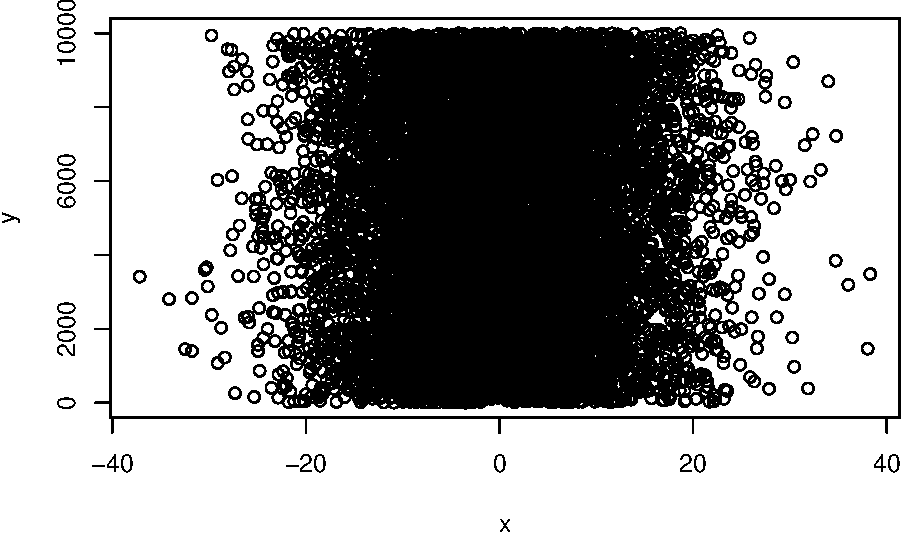
\includegraphics[width=1\linewidth]{foundational_statistics_files/figure-latex/Samples from distributions 1-1}

\begin{itemize}
\item
  You've probably figured out that ``y'' from the last example is a draw of numbers with equal probability (what we call a flat, or uniform distribution).
\item
  What if you want to draw from a defined probability distribution, like the normal distribution?
\item
  Again, play around with the arguments in the parentheses to see what happens.
\end{itemize}

\begin{Shaded}
\begin{Highlighting}[]
\NormalTok{x <-}\KeywordTok{rnorm}\NormalTok{(}\DecValTok{100}\NormalTok{, }\DecValTok{0}\NormalTok{, }\DecValTok{100}\NormalTok{)}
\KeywordTok{print}\NormalTok{ (x)}
\end{Highlighting}
\end{Shaded}

\begin{verbatim}
##   [1]    8.460665 -126.697188   92.839478  -31.683552   83.329877  -69.532089
##   [7]  -36.337099   76.410648   60.935949   56.902512   32.582157  -23.450918
##  [13] -168.371785  175.832658   29.585691  -59.601834 -123.840745 -101.168021
##  [19]   63.274650   23.048892   13.689664  -16.063567   71.293489 -102.179689
##  [25]  -71.009596  242.776533   56.783879  -12.282122  210.514667  232.338401
##  [31]  217.164077   84.403648   34.538762  -77.342504 -134.646162    4.286997
##  [37]  152.668741   62.782617   53.568224  -45.585819  -23.904039   36.960814
##  [43] -100.503491  177.150379   56.803961  -21.930267   39.165201  -64.884430
##  [49]  -23.022014   75.134345 -111.278021   16.489528  -43.981340  149.801960
##  [55]   78.334402  212.926380    7.166463  -50.106649  111.919641  -23.482962
##  [61]   25.023121 -103.817586  132.230895 -106.435630  -39.827578 -122.362532
##  [67] -130.581473   -8.899817   19.657763 -115.334426  -23.372908 -116.669382
##  [73]   44.311720 -133.110356  -50.138203  -53.097660 -130.489203   -2.196779
##  [79] -105.452035 -109.324568  -78.824243  101.486558 -101.119345  191.676368
##  [85]   -5.117758   55.791263 -141.325082 -262.512847  132.368976  -54.570877
##  [91]   14.363392  183.213184   39.375646  -48.682845    5.242619   11.974645
##  [97] -148.767940   18.599886  -70.743124 -270.915642
\end{verbatim}

\begin{Shaded}
\begin{Highlighting}[]
\KeywordTok{hist}\NormalTok{(x, }\DataTypeTok{xlim =} \KeywordTok{c}\NormalTok{(}\OperatorTok{-}\DecValTok{50}\NormalTok{,}\DecValTok{50}\NormalTok{))}
\end{Highlighting}
\end{Shaded}

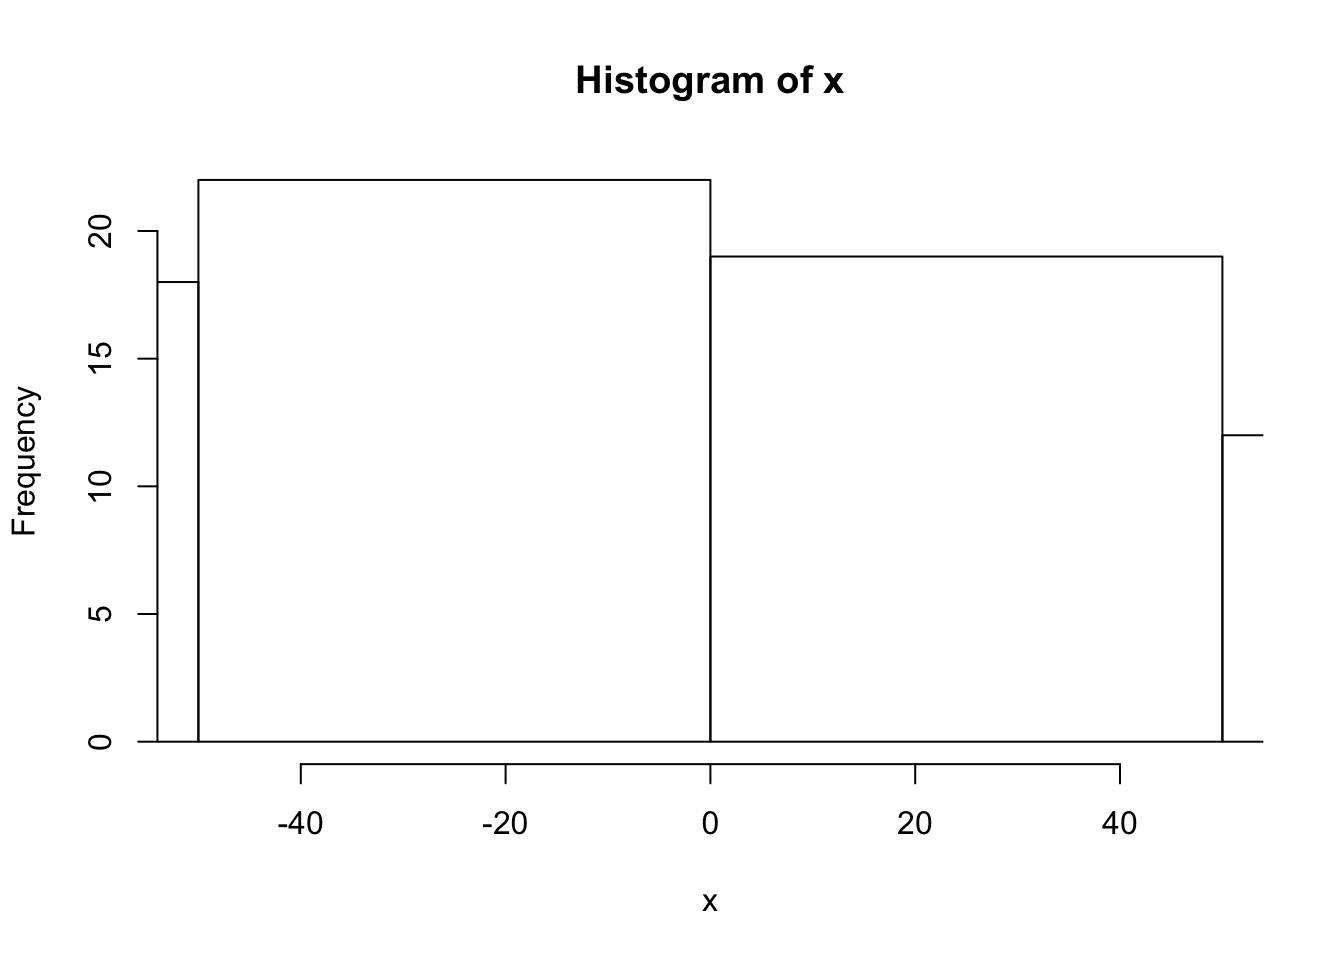
\includegraphics[width=1\linewidth]{foundational_statistics_files/figure-latex/Samples from distributions 2-1}

\begin{Shaded}
\begin{Highlighting}[]
\KeywordTok{hist}\NormalTok{(x, }\DataTypeTok{xlim =} \KeywordTok{c}\NormalTok{(}\OperatorTok{-}\DecValTok{500}\NormalTok{,}\DecValTok{500}\NormalTok{))}
\end{Highlighting}
\end{Shaded}

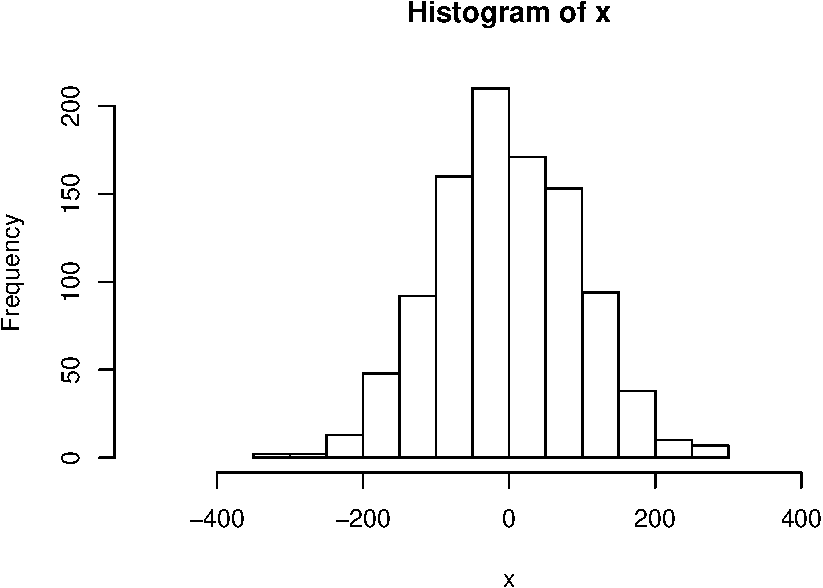
\includegraphics[width=1\linewidth]{foundational_statistics_files/figure-latex/Samples from distributions 2-2}

Can you figure out what the three rnorm() arguments represent?

\hypertarget{basic-summary-statistics}{%
\subsubsection{Basic Summary Statistics}\label{basic-summary-statistics}}

We will get into the details regarding summary statistics later, but for now, check out several of the \texttt{R} functions that calculate them.

\begin{Shaded}
\begin{Highlighting}[]
\KeywordTok{mean}\NormalTok{(x)}
\KeywordTok{median}\NormalTok{(x)}
\KeywordTok{var}\NormalTok{(x)}
\KeywordTok{log}\NormalTok{(x)}
\KeywordTok{ln}\NormalTok{(x)}
\KeywordTok{sqrt}\NormalTok{(x)}
\KeywordTok{sum}\NormalTok{(x)}
\KeywordTok{length}\NormalTok{(x)}
\KeywordTok{sample}\NormalTok{(x, }\DataTypeTok{replace =}\NormalTok{ T)}
\end{Highlighting}
\end{Shaded}

\begin{itemize}
\item
  Notice that the last function (\texttt{sample}) has an argument (\texttt{replace=T})
\item
  Arguments simply modify or direct the function in some way
\item
  There are many arguments for each function, some of which are defaults
\end{itemize}

\hypertarget{getting-help-to-understand-functions}{%
\subsubsection{Getting help to understand functions}\label{getting-help-to-understand-functions}}

\begin{itemize}
\item
  Getting help on any function is very easy - just type a question mark and the name of the function.
\item
  There are functions for just about anything within \texttt{R} and it is easy enough to write your own functions if none already exist to do what you want to do.
\item
  In general, function calls have a simple structure: a function name, a set of parentheses and an optional set of arguments you assign parameters to and send to the function.
\item
  Help pages exist for all functions that, at a minimum, explain what parameters exist for the function.
\item
  Help can be accessed a few ways - try them :
\end{itemize}

\begin{Shaded}
\begin{Highlighting}[]
\OperatorTok{-}\StringTok{ }\KeywordTok{help}\NormalTok{(mean)}
\OperatorTok{-}\StringTok{ }\NormalTok{?mean}
\OperatorTok{-}\StringTok{ }\KeywordTok{example}\NormalTok{(mean)}
\OperatorTok{-}\StringTok{ }\KeywordTok{help.search}\NormalTok{(}\StringTok{"mean"}\NormalTok{)}
\OperatorTok{-}\StringTok{ }\KeywordTok{apropos}\NormalTok{(}\StringTok{"mean"}\NormalTok{)}
\OperatorTok{-}\StringTok{ }\KeywordTok{args}\NormalTok{(mean)}
\end{Highlighting}
\end{Shaded}

\hypertarget{exercises-associated-with-this-chapter-1}{%
\section{Exercises associated with this chapter:}\label{exercises-associated-with-this-chapter-1}}

\begin{itemize}
\tightlist
\item
  Exercise 2 (\texttt{rtutorial\_1} in \texttt{foundstats} R package)
\end{itemize}

\hypertarget{additional-learning-resources-1}{%
\section{Additional learning resources:}\label{additional-learning-resources-1}}

\begin{itemize}
\item
  Logan, M. 2010. Biostatistical Design and Analysis Using R. - A great intro to R for statistical analysis
\item
  \url{http://library.open.oregonstate.edu/computationalbiology/} - O'Neil, S.T. 2017. A Primer for Computational Biology
\end{itemize}

\hypertarget{more-r-functions-complex-objects-basic-plotting-and-rmarkdown}{%
\chapter{More R Functions, Complex Objects, Basic Plotting, and RMarkdown}\label{more-r-functions-complex-objects-basic-plotting-and-rmarkdown}}

\hypertarget{background-1}{%
\section{Background}\label{background-1}}

In this chapter we will cover a variety of topics, all of which will help you build your \texttt{R} programming skills and make you capable of dealing with data sets using \texttt{R}. We will explore additional base \texttt{R} functions that are extremely useful for generating and manipulating vectors, combining vectors into multidimensional \texttt{R} objects, and working with those objects. We will also cover base \texttt{R} plotting functions to get you started with making your own publication-quality plots. Finally, we will touch on the RMarkdown file format, how to write those files in \texttt{RStudio}, and how to render the \texttt{.Rmd} file into polished, readable \texttt{.html} documents.

\hypertarget{more-on-functions}{%
\section{More on functions}\label{more-on-functions}}

In the last chapter we touched on functions in \texttt{R}, gave a few examples of commonly used functions, and covered how to learn more about a function using the \texttt{help()} function. As mentioned, functions and their use follow a basic structure. To call functions we type their name and include a set of parameters expressed as arguments, which specify what we want them to do, inside parentheses \texttt{()}. For example, to successfully call the function \texttt{mean()}, we need, at minimum, to supply a vector of numeric values. That vector can be an obect we have already assigned in our environment, or it can be the outcome of another function called within the \texttt{mean()} function. Below are these two alternatives.

\begin{Shaded}
\begin{Highlighting}[]
\NormalTok{z <-}\StringTok{ }\KeywordTok{c}\NormalTok{(}\DecValTok{10}\NormalTok{, }\DecValTok{20}\NormalTok{, }\DecValTok{30}\NormalTok{)}
\KeywordTok{mean}\NormalTok{(z)}
\end{Highlighting}
\end{Shaded}

\begin{verbatim}
## [1] 20
\end{verbatim}

\begin{Shaded}
\begin{Highlighting}[]
\KeywordTok{mean}\NormalTok{(}\KeywordTok{c}\NormalTok{(}\DecValTok{10}\NormalTok{, }\DecValTok{20}\NormalTok{, }\DecValTok{30}\NormalTok{))}
\end{Highlighting}
\end{Shaded}

\begin{verbatim}
## [1] 20
\end{verbatim}

The second alternative illustrates the power of ``nesting'' functions within \texttt{R}. You don't need to perform tasks by defining a bunch of intermediate objects and calling functions in piecemeal manner. In many cases it is much more efficient to nest functions within one another, as long as it doesn't jeopardize the functionality or readability of your code.

Base \texttt{R} includes dozens of useful functions that will become part of your regular arsenal. We have already mentioned several of these and discussed how to discover and learn more about them. As you become a more advanced \texttt{R} user, and in particular as you begin performing tasks and analyses more specific to your field of study, you will need to use functions that are not included in the base \texttt{R} library. Fortunately, there are thousands of functions distributed in the form of \texttt{R} ``packages,'' which you can easily install on your system. Packages especially easy to find and use are those distributed via the Comprehensive R Archive Network (CRAN): \url{https://cran.r-project.org/web/packages/index.html}. If you find a specific function or set of functions you are interested in trying out, for instance after a Google search of your problem, you can download and install the package those functions belong to by running the following command from your \texttt{R} Console:

\begin{Shaded}
\begin{Highlighting}[]
\KeywordTok{install.packages}\NormalTok{(}\StringTok{"name_of_package"}\NormalTok{)}
\end{Highlighting}
\end{Shaded}

Note that the name of the package has to be spelled correctly (and \texttt{R} is case sensitive), and that the name of the package should be in quotation marks. You will get a series of messages printed to the Console, and finally either a confirmation of installation or error message. Once you have installed a package successfully, you do not need to re-run the \texttt{install.packages()} function. If you want to check whether a package has already been installed, and look at the details of that installation, you can always run the following from the Console:

\begin{Shaded}
\begin{Highlighting}[]
\KeywordTok{installed.packages}\NormalTok{(}\StringTok{"name_of_package"}\NormalTok{)}
\end{Highlighting}
\end{Shaded}

To actually use the functions from an installed package, you have to ``load'' that package into your current working environment. To do that we use the \texttt{library()} function:

\begin{Shaded}
\begin{Highlighting}[]
\KeywordTok{library}\NormalTok{(name_of_package)}
\end{Highlighting}
\end{Shaded}

Note that you do not include quotation marks around the package name for the \texttt{library()} function. Unlike package installation, you will need to invoke \texttt{library()} every time you start a new \texttt{R} session to load the package and its functions.

It is also possible, and quite straightforward, to write your own \texttt{R} functions, which you can define within your \texttt{.R} or \texttt{.Rmd} scripts for convenient usage. If you get the the point at which you want to distribute your own functions in the form of a package, that is possible too. Later during this course we will get a little experience in writing simple \texttt{R} functions. Writing more involved functions and publishing packages, however, are topics for a more advanced \texttt{R} course.

\hypertarget{more-base-r-functions-useful-for-working-with-vectors}{%
\subsection{\texorpdfstring{More base \texttt{R} functions useful for working with vectors}{More base R functions useful for working with vectors}}\label{more-base-r-functions-useful-for-working-with-vectors}}

Below are annotated lists of base \texttt{R} functions commonly used to work with vectors. We will not take the time here to give specific examples for each function, because their usage is quite straightforward and you will get plenty of practice with them in associated exercies. You can also practice using the \texttt{help()} function if you have specific questions.

\textbf{The following functions provide information about vectors:}

\begin{itemize}
\item
  \texttt{head()}: returns the first elements of an object (like a vector or data frame)
\item
  \texttt{tail()}: returns the last elements of an object (like a vector or data frame)
\item
  \texttt{length()}: returns the number of elements in a vector
\item
  \texttt{class()}: returns the class of elements in a vector (e.g. ``character'', ``numeric'', ``factor'', etc.)
\end{itemize}

\textbf{The following functions can modify or generate vectors in structured ways:}

\begin{itemize}
\item
  \texttt{sort()}: returns a sorted vector from an orignal vector of numeric values
\item
  \texttt{seq()}: returns a ``series'' of numeric values beginning at one value and ending at another, while also specifying the size of increments/decrements between values
\item
  \texttt{rep()}: returns a vector of identical elements, repeated a specified number of times
\end{itemize}

\begin{Shaded}
\begin{Highlighting}[]
\KeywordTok{rep}\NormalTok{(}\DecValTok{1}\NormalTok{, }\DecValTok{5}\NormalTok{)}
\end{Highlighting}
\end{Shaded}

\begin{verbatim}
## [1] 1 1 1 1 1
\end{verbatim}

\begin{Shaded}
\begin{Highlighting}[]
\KeywordTok{rep}\NormalTok{(}\StringTok{"one"}\NormalTok{, }\DecValTok{5}\NormalTok{)}
\end{Highlighting}
\end{Shaded}

\begin{verbatim}
## [1] "one" "one" "one" "one" "one"
\end{verbatim}

Note that \texttt{seq()} and \texttt{rep()} can be repeated and/or combined in various ways, in some cases using \texttt{c()}, to generate vectors in a multitude of patterned ways.

\textbf{The following functions can generate vectors of random values, randomly shuffle vectors, or generate vectors of values drawn from defined probability distributions:}

\begin{itemize}
\item
  \texttt{sample()}: randomly selects and returns elements from a vector (``shuffles'' a vector when size argument is set to original vector size and replace argument is set to ``FALSE'')
\item
  \texttt{rnorm()}: randomly draws values from a theoretical normal distribution
\item
  \texttt{rbinom()}: randomly draws values from a theoretical binomial distribution
\item
  \texttt{set.seed()}: sets \texttt{R}'s random number generator seed so that operations with stochastic properties can be reproduced
\end{itemize}

\textbf{The following functions can change the class of elements in a particular vector:}

\begin{itemize}
\item
  \texttt{as.numeric()}: changes the class of objects in a vector to ``numeric''.
\item
  \texttt{as.factor()}: changes the class of objects in a vector to ``factor''.
\item
  \texttt{as.character()}: changes the class of objects in a vector to ``character''.
\end{itemize}

The \texttt{as.xxx} family of \texttt{R} functions is especially useful if you need to convert the class of a particular object for a given function to use the object properly.

\hypertarget{indexing-vectors}{%
\section{Indexing vectors}\label{indexing-vectors}}

Now that we are quite familiar with different ways for generating vectors, let's discuss how we isolate specific elements from those vectors. This process is called ``indexing,'' and in \texttt{R} simple numeric (or ``positional'') indexing is intuitively based on integers, starting from ``1''. We use the square braces for numeric indexing in \texttt{R}: \texttt{{[}{]}}. For example if we want to index the first element in a vector, we simply type \texttt{{[}1{]}} after the vector. Indexing can be performed on a defined vector, or on the fly using the immediate output of a function call.

\begin{Shaded}
\begin{Highlighting}[]
\CommentTok{## Using our vector z from above}
\NormalTok{z[}\DecValTok{1}\NormalTok{]}
\end{Highlighting}
\end{Shaded}

\begin{verbatim}
## [1] 10
\end{verbatim}

\begin{Shaded}
\begin{Highlighting}[]
\CommentTok{## On the fly using output from the c() function}
\KeywordTok{c}\NormalTok{(}\DecValTok{10}\NormalTok{, }\DecValTok{20}\NormalTok{, }\DecValTok{30}\NormalTok{)[}\DecValTok{1}\NormalTok{]}
\end{Highlighting}
\end{Shaded}

\begin{verbatim}
## [1] 10
\end{verbatim}

To isolate a series of consecutive elements from a vector, we simply use the \texttt{:} character. For example, if we want to index the first (or last) 4 elements from the vector below we could do this, respectively:

\begin{Shaded}
\begin{Highlighting}[]
\KeywordTok{c}\NormalTok{(}\DecValTok{10}\NormalTok{, }\DecValTok{20}\NormalTok{, }\DecValTok{30}\NormalTok{, }\DecValTok{40}\NormalTok{, }\DecValTok{50}\NormalTok{, }\DecValTok{100}\NormalTok{, }\DecValTok{200}\NormalTok{)[}\DecValTok{1}\OperatorTok{:}\DecValTok{4}\NormalTok{]}
\end{Highlighting}
\end{Shaded}

\begin{verbatim}
## [1] 10 20 30 40
\end{verbatim}

\begin{Shaded}
\begin{Highlighting}[]
\KeywordTok{c}\NormalTok{(}\DecValTok{10}\NormalTok{, }\DecValTok{20}\NormalTok{, }\DecValTok{30}\NormalTok{, }\DecValTok{40}\NormalTok{, }\DecValTok{50}\NormalTok{, }\DecValTok{100}\NormalTok{, }\DecValTok{200}\NormalTok{)[}\DecValTok{4}\OperatorTok{:}\DecValTok{7}\NormalTok{]}
\end{Highlighting}
\end{Shaded}

\begin{verbatim}
## [1]  40  50 100 200
\end{verbatim}

For indexing discontinuous elements, we can use our old friend, the \texttt{c()} function inside of the square braces. So, if we want to index the first 3 and the 5th elements:

\begin{Shaded}
\begin{Highlighting}[]
\KeywordTok{c}\NormalTok{(}\DecValTok{10}\NormalTok{, }\DecValTok{20}\NormalTok{, }\DecValTok{30}\NormalTok{, }\DecValTok{40}\NormalTok{, }\DecValTok{50}\NormalTok{, }\DecValTok{100}\NormalTok{, }\DecValTok{200}\NormalTok{)[}\KeywordTok{c}\NormalTok{(}\DecValTok{1}\OperatorTok{:}\DecValTok{3}\NormalTok{, }\DecValTok{5}\NormalTok{)]}
\end{Highlighting}
\end{Shaded}

\begin{verbatim}
## [1] 10 20 30 50
\end{verbatim}

Finally, we can use the \texttt{-} character to index all elements of a vector, ``minus'' other elements. When excluding even consecutive elements, however, we have to include \texttt{c()}. For instance, if we want all \textbf{except} the first 2 elements, we could do:

\begin{Shaded}
\begin{Highlighting}[]
\KeywordTok{c}\NormalTok{(}\DecValTok{10}\NormalTok{, }\DecValTok{20}\NormalTok{, }\DecValTok{30}\NormalTok{, }\DecValTok{40}\NormalTok{, }\DecValTok{50}\NormalTok{, }\DecValTok{100}\NormalTok{, }\DecValTok{200}\NormalTok{)[}\OperatorTok{-}\KeywordTok{c}\NormalTok{(}\DecValTok{1}\OperatorTok{:}\DecValTok{2}\NormalTok{)]}
\end{Highlighting}
\end{Shaded}

\begin{verbatim}
## [1]  30  40  50 100 200
\end{verbatim}

\hypertarget{more-complex-data-objects-in-r}{%
\section{\texorpdfstring{More complex data objects in \texttt{R}}{More complex data objects in R}}\label{more-complex-data-objects-in-r}}

Vectors are extremely important object types in \texttt{R}, for the reasons and examples we have already discussed. Other types of objects in \texttt{R} are also important, and necessary to learn about to do meaningful and efficient work. These other types of objects are more complex than vectors, but they can, in many cases, be composed of vectors.

\hypertarget{lists}{%
\subsection{lists}\label{lists}}

Lists in \texttt{R} are aggregates of different objects, and those objects can be a mixed variety of types. For example, a list could be an aggregate of 3 different vectors, even if those vectors are different lengths and contain elements of a different class. We can generate lists using the \texttt{list()} function.

\begin{Shaded}
\begin{Highlighting}[]
\NormalTok{vec1 <-}\StringTok{ }\KeywordTok{c}\NormalTok{(}\DecValTok{10}\NormalTok{, }\DecValTok{20}\NormalTok{, }\DecValTok{30}\NormalTok{, }\DecValTok{40}\NormalTok{, }\DecValTok{50}\NormalTok{, }\DecValTok{100}\NormalTok{, }\DecValTok{200}\NormalTok{)}
\NormalTok{vec2 <-}\StringTok{ }\KeywordTok{c}\NormalTok{(}\StringTok{"happy"}\NormalTok{, }\StringTok{"sad"}\NormalTok{, }\StringTok{"grumpy"}\NormalTok{)}
\NormalTok{vec3 <-}\StringTok{ }\KeywordTok{factor}\NormalTok{(}\KeywordTok{c}\NormalTok{(}\StringTok{"high"}\NormalTok{, }\StringTok{"low"}\NormalTok{))}

\NormalTok{mylist <-}\StringTok{ }\KeywordTok{list}\NormalTok{(vec1, vec2, vec3)}

\KeywordTok{print}\NormalTok{(mylist)}
\end{Highlighting}
\end{Shaded}

\begin{verbatim}
## [[1]]
## [1]  10  20  30  40  50 100 200
## 
## [[2]]
## [1] "happy"  "sad"    "grumpy"
## 
## [[3]]
## [1] high low 
## Levels: high low
\end{verbatim}

\begin{Shaded}
\begin{Highlighting}[]
\KeywordTok{class}\NormalTok{(mylist)}
\end{Highlighting}
\end{Shaded}

\begin{verbatim}
## [1] "list"
\end{verbatim}

\begin{Shaded}
\begin{Highlighting}[]
\KeywordTok{str}\NormalTok{(mylist)}
\end{Highlighting}
\end{Shaded}

\begin{verbatim}
## List of 3
##  $ : num [1:7] 10 20 30 40 50 100 200
##  $ : chr [1:3] "happy" "sad" "grumpy"
##  $ : Factor w/ 2 levels "high","low": 1 2
\end{verbatim}

Let's take note of a few things from the output above. First, notice that each of the three vectors in \texttt{mylist} has a numeric (positional) index. Unlike individual vectors, however, primary elements of lists are indexed by double square braces \texttt{{[}{[}{]}{]}}. So, if we want to index the \texttt{vec2} element of \texttt{mylist}, we type:

\begin{Shaded}
\begin{Highlighting}[]
\NormalTok{mylist[[}\DecValTok{2}\NormalTok{]]}
\end{Highlighting}
\end{Shaded}

\begin{verbatim}
## [1] "happy"  "sad"    "grumpy"
\end{verbatim}

Taking it one step further, if we want to index the 2nd element of the \texttt{vec2} element of \texttt{mylist}, we type:

\begin{Shaded}
\begin{Highlighting}[]
\NormalTok{mylist[[}\DecValTok{2}\NormalTok{]][}\DecValTok{2}\NormalTok{]}
\end{Highlighting}
\end{Shaded}

\begin{verbatim}
## [1] "sad"
\end{verbatim}

The other things we should note from our exploration of \texttt{mylist} above is that 1. It has a class when we call the \texttt{class()} function, and 2. We see a nice breakdown of the 3 components that make up \texttt{mylist} when we call the \texttt{str()} function. \texttt{str()}, which is short for ``structure,'' is an especially useful function for trying to understand the organization of complex objects in \texttt{R}.

\hypertarget{data-frames}{%
\subsection{data frames}\label{data-frames}}

There is a special class of list we very often work with in \texttt{R} called a ``data frame.'' You can think of data frames as an especially useful organizing structure for data sets. Data frames are lists of vectors, but the vectors have to be the same length. Also, the vectors (officially known as ``columns'') in data frames have names we refer to as ``column names,'' and the rows also have names. For the types of analysis we will be dealing with in this course, it helps to organize our data so that variables in our study correspond to columns and observations correspond to rows. Let's explore some practical details regarding the generation and use of data frames.

\hypertarget{creating-data-frames-in-r}{%
\subsubsection{\texorpdfstring{creating data frames in \texttt{R}}{creating data frames in R}}\label{creating-data-frames-in-r}}

We can generate data frames manually, like we did with the list \texttt{mylist} above. Here, for example, we can set up three variables (habitat, temp and elevation) as vectors.

\begin{Shaded}
\begin{Highlighting}[]
\NormalTok{habitat <-}\StringTok{ }\KeywordTok{factor}\NormalTok{(}\KeywordTok{c}\NormalTok{(}\StringTok{"mixed"}\NormalTok{, }\StringTok{"wet"}\NormalTok{, }\StringTok{"wet"}\NormalTok{, }\StringTok{"wet"}\NormalTok{, }\StringTok{"dry"}\NormalTok{, }\StringTok{"dry"}\NormalTok{, }\StringTok{"dry"}\NormalTok{,}\StringTok{"mixed"}\NormalTok{))}
\NormalTok{temp <-}\StringTok{ }\KeywordTok{c}\NormalTok{(}\FloatTok{3.4}\NormalTok{, }\FloatTok{3.4}\NormalTok{, }\FloatTok{8.4}\NormalTok{, }\DecValTok{3}\NormalTok{, }\FloatTok{5.6}\NormalTok{, }\FloatTok{8.1}\NormalTok{, }\FloatTok{8.3}\NormalTok{, }\FloatTok{4.5}\NormalTok{)}
\NormalTok{elevation <-}\StringTok{ }\KeywordTok{c}\NormalTok{(}\DecValTok{0}\NormalTok{, }\FloatTok{9.2}\NormalTok{, }\FloatTok{3.8}\NormalTok{, }\DecValTok{5}\NormalTok{, }\FloatTok{5.6}\NormalTok{, }\FloatTok{4.1}\NormalTok{, }\FloatTok{7.1}\NormalTok{, }\FloatTok{5.3}\NormalTok{)}
\end{Highlighting}
\end{Shaded}

Then we can use the \texttt{data.frame()} function to incorporate the vectors into columns of the data frame.

\begin{Shaded}
\begin{Highlighting}[]
\NormalTok{mydata <-}\StringTok{ }\KeywordTok{data.frame}\NormalTok{(habitat, temp, elevation)}
\KeywordTok{row.names}\NormalTok{(mydata) <-}\StringTok{ }\KeywordTok{c}\NormalTok{(}\StringTok{"Reedy Lake"}\NormalTok{, }\StringTok{"Pearcadale"}\NormalTok{, }\StringTok{"Warneet"}\NormalTok{, }\StringTok{"Cranbourne"}\NormalTok{, }
                       \StringTok{"Lysterfield"}\NormalTok{, }\StringTok{"Red Hill"}\NormalTok{, }\StringTok{"Devilbend"}\NormalTok{, }\StringTok{"Olinda"}\NormalTok{)}
\end{Highlighting}
\end{Shaded}

Note above that we used a function called \texttt{row.names} to assign row names to \texttt{mydata}. The function \texttt{colnames()} does the same, but for column names.

\hypertarget{working-with-pre-loaded-base-r-data-frames.}{%
\subsubsection{\texorpdfstring{working with pre-loaded base \texttt{R} data frames.}{working with pre-loaded base R data frames.}}\label{working-with-pre-loaded-base-r-data-frames.}}

There are a few data frames that are available to work with whenever you begin an \texttt{R} session. These can be a great way to practice plotting and analysis, and in fact many examples written to accompany \texttt{R} functions include these data frames to promote reproducibility and convenience. Two of these pre-loaded data frames that are especially popular are \texttt{mtcars} and \texttt{iris}.

\begin{Shaded}
\begin{Highlighting}[]
\KeywordTok{head}\NormalTok{(mtcars)}
\end{Highlighting}
\end{Shaded}

\begin{verbatim}
##                    mpg cyl disp  hp drat    wt  qsec vs am gear carb
## Mazda RX4         21.0   6  160 110 3.90 2.620 16.46  0  1    4    4
## Mazda RX4 Wag     21.0   6  160 110 3.90 2.875 17.02  0  1    4    4
## Datsun 710        22.8   4  108  93 3.85 2.320 18.61  1  1    4    1
## Hornet 4 Drive    21.4   6  258 110 3.08 3.215 19.44  1  0    3    1
## Hornet Sportabout 18.7   8  360 175 3.15 3.440 17.02  0  0    3    2
## Valiant           18.1   6  225 105 2.76 3.460 20.22  1  0    3    1
\end{verbatim}

\begin{Shaded}
\begin{Highlighting}[]
\KeywordTok{head}\NormalTok{(iris)}
\end{Highlighting}
\end{Shaded}

\begin{verbatim}
##   Sepal.Length Sepal.Width Petal.Length Petal.Width Species
## 1          5.1         3.5          1.4         0.2  setosa
## 2          4.9         3.0          1.4         0.2  setosa
## 3          4.7         3.2          1.3         0.2  setosa
## 4          4.6         3.1          1.5         0.2  setosa
## 5          5.0         3.6          1.4         0.2  setosa
## 6          5.4         3.9          1.7         0.4  setosa
\end{verbatim}

\hypertarget{reading-in-data-frames-in-r}{%
\subsubsection{\texorpdfstring{reading in data frames in \texttt{R}}{reading in data frames in R}}\label{reading-in-data-frames-in-r}}

A strength of \texttt{R} is being able to import data from an external source. For example, if you have a comma- or tab- separated text file (like the UNIX-friendly formats we discussed previously), it can be easily read into \texttt{R}, by default as a data frame. One function for accomplishing this is \texttt{read.table()}, although functions like \texttt{read.delim()} can be similarly applied. Two important arguments for \texttt{read.table()} are ``header'' and ``row.names'', which indicate that there is a header row (with column names) and row label column (with row names), respectively. You also need to supply the file path and name in quotation marks (no path necessary if the file is in the current working directory), and what character is used as the field (column) delimiter. Here is an example:

\begin{Shaded}
\begin{Highlighting}[]
\NormalTok{YourFile <-}\StringTok{ }\KeywordTok{read.table}\NormalTok{(}\StringTok{'yourfile.csv'}\NormalTok{, }\DataTypeTok{header=}\NormalTok{T, }\DataTypeTok{row.names=}\DecValTok{1}\NormalTok{, }\DataTypeTok{sep=}\StringTok{','}\NormalTok{)}
\NormalTok{YourFile <-}\StringTok{ }\KeywordTok{read.table}\NormalTok{(}\StringTok{'yourfile.txt'}\NormalTok{, }\DataTypeTok{header=}\NormalTok{T, }\DataTypeTok{row.names=}\DecValTok{1}\NormalTok{, }\DataTypeTok{sep=}\StringTok{'}\CharTok{\textbackslash{}t}\StringTok{'}\NormalTok{)}
\end{Highlighting}
\end{Shaded}

\hypertarget{exporting-data-frames-in-r}{%
\subsubsection{\texorpdfstring{exporting data frames in \texttt{R}}{exporting data frames in R}}\label{exporting-data-frames-in-r}}

If you ever want to save a data frame in a format that you can work with outside of \texttt{R}, the \texttt{write.table()} function does pretty much the opposite of its ``read'' counterpart.

\begin{Shaded}
\begin{Highlighting}[]
\KeywordTok{write.table}\NormalTok{(YourFile, }\StringTok{"yourfile.csv"}\NormalTok{, }\DataTypeTok{quote=}\NormalTok{F, }\DataTypeTok{row.names=}\NormalTok{T, }\DataTypeTok{sep=}\StringTok{","}\NormalTok{)}
\KeywordTok{write.table}\NormalTok{(YourFile, }\StringTok{"yourfile.txt"}\NormalTok{, }\DataTypeTok{quote=}\NormalTok{F, }\DataTypeTok{row.names=}\NormalTok{T, }\DataTypeTok{sep=}\StringTok{"}\CharTok{\textbackslash{}t}\StringTok{"}\NormalTok{)}
\end{Highlighting}
\end{Shaded}

\hypertarget{indexing-data-frames}{%
\subsubsection{indexing data frames}\label{indexing-data-frames}}

Indexing data frames can be acheived in two different ways. We can use numeric (positional) indexing as in the case of vectors and lists (see above). With a data frame, we can index any subset of it using two pieces of information: row coordinates and column coordinates. To accomplish this we use single square braces \texttt{{[},{]}}, in which the row coordinate(s) are typed first, followed by a comma, followed by the column cooridate(s). If we want to index all rows or all columns, we just leave the space to the left or right of the comma blank, respectively. Here are some examples for indexing subsets of the \texttt{iris} data frame.

\begin{Shaded}
\begin{Highlighting}[]
\CommentTok{## The first row, with all columns}
\NormalTok{iris[}\DecValTok{1}\NormalTok{,]}
\end{Highlighting}
\end{Shaded}

\begin{verbatim}
##   Sepal.Length Sepal.Width Petal.Length Petal.Width Species
## 1          5.1         3.5          1.4         0.2  setosa
\end{verbatim}

\begin{Shaded}
\begin{Highlighting}[]
\CommentTok{## The first 5 rows and the first 2 columns}
\NormalTok{iris[}\DecValTok{1}\OperatorTok{:}\DecValTok{5}\NormalTok{,}\DecValTok{1}\OperatorTok{:}\DecValTok{2}\NormalTok{]}
\end{Highlighting}
\end{Shaded}

\begin{verbatim}
##   Sepal.Length Sepal.Width
## 1          5.1         3.5
## 2          4.9         3.0
## 3          4.7         3.2
## 4          4.6         3.1
## 5          5.0         3.6
\end{verbatim}

With data frames, we can also use the column names to index subsets. To do this we use the \texttt{\$} character after the name of the data frame, followed by the name of the column we want to index. Again, below is a demonstration using \texttt{iris}. Indexing using column names is perhaps the most useful when defining statistical models, a topic we will reach later in the course.

\begin{Shaded}
\begin{Highlighting}[]
\CommentTok{## The first 5 rows of the first column}
\NormalTok{iris}\OperatorTok{$}\NormalTok{Sepal.Length[}\DecValTok{1}\OperatorTok{:}\DecValTok{5}\NormalTok{]}
\end{Highlighting}
\end{Shaded}

\begin{verbatim}
## [1] 5.1 4.9 4.7 4.6 5.0
\end{verbatim}

\hypertarget{matrices}{%
\subsection{matrices}\label{matrices}}

Matrices in \texttt{R} are somewhat similar to data frames, but mixed classes among columns are not permitted, and rows and columns are only positionally indexed as opposed to having names. Positional indexing for matrices, not surprisingly, follows the \texttt{{[}rownumber,\ columnnumber{]}} convention, similar to data frames. A matrix can be generated using the \texttt{matrix()} function, as demonstrated below.

\begin{Shaded}
\begin{Highlighting}[]
\CommentTok{## Populate a 3x3 matrix with values 1 to 9}
\KeywordTok{matrix}\NormalTok{(}\DecValTok{1}\OperatorTok{:}\DecValTok{9}\NormalTok{, }\DataTypeTok{nrow=}\DecValTok{3}\NormalTok{, }\DataTypeTok{ncol=}\DecValTok{3}\NormalTok{)}
\end{Highlighting}
\end{Shaded}

\begin{verbatim}
##      [,1] [,2] [,3]
## [1,]    1    4    7
## [2,]    2    5    8
## [3,]    3    6    9
\end{verbatim}

\hypertarget{a-few-additional-base-r-functions-for-working-with-complex-r-objects}{%
\subsection{\texorpdfstring{A few additional base \texttt{R} functions for working with complex \texttt{R} objects}{A few additional base R functions for working with complex R objects}}\label{a-few-additional-base-r-functions-for-working-with-complex-r-objects}}

To add to your foundational knowledge of \texttt{R} functions, below are a few more functions especially useful for working with objects like data frames and matrices.

\begin{itemize}
\item
  \texttt{dim()}: returns the number of rows and columns of a data frame or matrix
\item
  \texttt{View()}: opens up a GUI ``viewer'' for visual inspection of data frames (not recommended for large data frames)
\item
  \texttt{cbind()}: combines columns into a single object, which can be used to define or build data frames or matrices
\item
  \texttt{rbind()}: combines rows into a single object, which can be used to define or build data frames or matrices
\item
  \texttt{t()}: transposes a data frame or matrix, such that rows become columns, and columns become rows
\end{itemize}

\hypertarget{some-brief-notes-on-basic-programming-in-r}{%
\section{\texorpdfstring{Some brief notes on basic programming in \texttt{R}}{Some brief notes on basic programming in R}}\label{some-brief-notes-on-basic-programming-in-r}}

At some point during your development as an \texttt{R} user you will want to programmatically manipulate \texttt{R} objects in an iterative, repeatable manner to automate tasks like plotting, simulations, and analysis. This use of the \texttt{R} language is especially relevant if you want to write your own functions. Here we touch on a few tools and approaches that will open the door to more powerful programming in \texttt{R}. These are skills that are great to practice and learn, but at a fairly foundational level for now. More advanced programming training in \texttt{R} is beyond the scope of this course.

\hypertarget{conditional-statements-with-ifelse}{%
\subsection{\texorpdfstring{conditional statements with \texttt{ifelse()}}{conditional statements with ifelse()}}\label{conditional-statements-with-ifelse}}

One fundamental structural component of computer programming languages is the idea of conditional statements, which often take the form of ``if/else'' evaluation and execution. The idea is that we can write an algorithm to evaluate a particular statement using a logical operator, and if that statement is true have the program do one thing, but if the statement is false, have it do somehting ``else.'' In \texttt{R} we can write these statements with a structure similar to other languages, but we can also use the single \texttt{R} function \texttt{ifelse()} to accomplish the same thing. The \texttt{ifelse()} function is very easy to use. The first argument is the logical evaluation, the second argument is the action to take if that statement is true, and the third argument is the action to take if false. It is also possible to nest multiple \texttt{ifelse()} function calls wihtin one another, if mulitiple evaluations need to be performed with different outcomes. Below is a simple example for using \texttt{ifelse()} to generate a vector of values (``colors''), based on another vector.

\begin{Shaded}
\begin{Highlighting}[]
\CommentTok{## First define a character vector}
\NormalTok{char_vec <-}\StringTok{ }\KeywordTok{c}\NormalTok{(}\KeywordTok{rep}\NormalTok{(}\StringTok{"treatment"}\NormalTok{,}\DecValTok{5}\NormalTok{), }\KeywordTok{rep}\NormalTok{(}\StringTok{"control"}\NormalTok{,}\DecValTok{3}\NormalTok{), }\KeywordTok{rep}\NormalTok{(}\StringTok{"treatment"}\NormalTok{, }\DecValTok{4}\NormalTok{), }\KeywordTok{rep}\NormalTok{(}\StringTok{"control"}\NormalTok{, }\DecValTok{6}\NormalTok{))}
\KeywordTok{print}\NormalTok{(char_vec)}
\end{Highlighting}
\end{Shaded}

\begin{verbatim}
##  [1] "treatment" "treatment" "treatment" "treatment" "treatment" "control"  
##  [7] "control"   "control"   "treatment" "treatment" "treatment" "treatment"
## [13] "control"   "control"   "control"   "control"   "control"   "control"
\end{verbatim}

\begin{Shaded}
\begin{Highlighting}[]
\CommentTok{## Generate a vector that stores the color "red" for "treatment" and "blue" for "control"}
\NormalTok{col_vec <-}\StringTok{ }\KeywordTok{ifelse}\NormalTok{(char_vec}\OperatorTok{==}\StringTok{"treatment"}\NormalTok{, }\StringTok{"red"}\NormalTok{, }\StringTok{"blue"}\NormalTok{)}
\KeywordTok{print}\NormalTok{(col_vec)}
\end{Highlighting}
\end{Shaded}

\begin{verbatim}
##  [1] "red"  "red"  "red"  "red"  "red"  "blue" "blue" "blue" "red"  "red" 
## [11] "red"  "red"  "blue" "blue" "blue" "blue" "blue" "blue"
\end{verbatim}

\hypertarget{replicate-tapply-and-apply}{%
\subsection{\texorpdfstring{\texttt{replicate()}, \texttt{tapply()}, and \texttt{apply()}}{replicate(), tapply(), and apply()}}\label{replicate-tapply-and-apply}}

In some cases we want to repeat a given process over and over again. For example, maybe we want to simulate the sampling process and generate 100 random samples of 100 values from a normal distribution. Fortunately, the \texttt{R} function \texttt{replicate()} makes this very easy.

In the example below, we ``shuffle'' the order of the integers 1 through 10 five times using \texttt{replicate()}:

\begin{Shaded}
\begin{Highlighting}[]
\KeywordTok{replicate}\NormalTok{(}\DecValTok{5}\NormalTok{, }\KeywordTok{sample}\NormalTok{(}\DecValTok{1}\OperatorTok{:}\DecValTok{10}\NormalTok{, }\DataTypeTok{size=}\DecValTok{10}\NormalTok{, }\DataTypeTok{replace=}\OtherTok{FALSE}\NormalTok{))}
\end{Highlighting}
\end{Shaded}

\begin{verbatim}
##       [,1] [,2] [,3] [,4] [,5]
##  [1,]    7    4    7   10    1
##  [2,]    3    8    9    2    3
##  [3,]    2    5    1    6   10
##  [4,]    9    9    5    7    5
##  [5,]    6    2   10    9    9
##  [6,]    8   10    6    4    8
##  [7,]   10    6    3    3    6
##  [8,]    1    1    8    1    4
##  [9,]    5    3    2    5    2
## [10,]    4    7    4    8    7
\end{verbatim}

Note that the first argument is the number of total iterations we want to reproduce, and that the function returns a matrix as output.

The \texttt{replicate()} function belongs to a group of functions referred to informally as the ``apply'' family. Another commonly used function from this group is \texttt{tapply()}, which allows you to apply a function to one vector (for example a numeric vector in a data frame), in a group-wise manner based on one or more factor vectors that correspond to the numeric vector. In other words, if we want to find the maximum value of variable x for each level of factor y in a data frame, we could use \texttt{tapply()} to do so. Below is an example, again using the \texttt{iris} data frame.

\begin{Shaded}
\begin{Highlighting}[]
\CommentTok{## Find the maximum petal length for each species in the iris data frame}
\KeywordTok{tapply}\NormalTok{(iris}\OperatorTok{$}\NormalTok{Petal.Length, iris}\OperatorTok{$}\NormalTok{Species, max)}
\end{Highlighting}
\end{Shaded}

\begin{verbatim}
##     setosa versicolor  virginica 
##        1.9        5.1        6.9
\end{verbatim}

Note that the first argument is the numerical column, and the second is a factor column. The third is the function we wish to apply, in this case to each species separately.

Another, similar function from this family is simply called \texttt{apply()}, and it can be used to apply a function to either all rows (with the MARGIN argument set to 1) or all columns (with the MARGIN argument set to 2) in a data frame or matrix. This is especially useful for calculating summary statistics for what we call the ``margins'' of data in tables.

\hypertarget{for-loops-in-r}{%
\subsection{\texorpdfstring{for loops in \texttt{R}}{for loops in R}}\label{for-loops-in-r}}

Another fundamental concept in computer programming is the ``for loop,'' which is an algorithmic strategy for iteratively performing a task according to a pre-defined counter or loop variable, then terminating when the ``loop'' is evaluated as complete. For example, we may want to perform a specific calculation again and again for sucessive elements of an \texttt{R} object (like a data frame), and build a vector that successively stores the calculation for each iteration of the ``loop.'' We will not devote much time to for loops in \texttt{R} here, because the ``apply'' group of functions can accomplish many of the tasks you would write a for loop to perform, with much greater speed. If you do find a need for including a for loop in your future \texttt{R} programming, however, the commented example below illustrates an efficient framework in which ``pre-allocation'' of an output vector maximizes for loop speed despite some of \texttt{R}'s.

\begin{Shaded}
\begin{Highlighting}[]
\CommentTok{## Calculate mpg/cyl and mpg/wt, for every row in mtcars and if the second is at least twice the size of the first include that ratio and another character value "Yes" in a growing 2-column dataframe. If the ratio is less than 2, then include "No" in the second column. }

\CommentTok{## first pre-allocate our new data frame, which contains NAs initially}
\NormalTok{newdf <-}\StringTok{ }\KeywordTok{data.frame}\NormalTok{(}\KeywordTok{rep}\NormalTok{(}\OtherTok{NA}\NormalTok{, }\KeywordTok{length}\NormalTok{(mtcars}\OperatorTok{$}\NormalTok{mpg)), }\KeywordTok{rep}\NormalTok{(}\OtherTok{NA}\NormalTok{, }\KeywordTok{length}\NormalTok{(mtcars}\OperatorTok{$}\NormalTok{mpg)))}

\CommentTok{## then write the for loop to do the above task for every row in mtcars}
\ControlFlowTok{for}\NormalTok{(i }\ControlFlowTok{in} \DecValTok{1}\OperatorTok{:}\KeywordTok{length}\NormalTok{(mtcars}\OperatorTok{$}\NormalTok{mpg)) \{}
\NormalTok{  newdf[i,}\DecValTok{1}\NormalTok{] <-}\StringTok{ }\NormalTok{(mtcars}\OperatorTok{$}\NormalTok{mpg[i]}\OperatorTok{/}\NormalTok{mtcars}\OperatorTok{$}\NormalTok{wt[i])}\OperatorTok{/}\NormalTok{(mtcars}\OperatorTok{$}\NormalTok{mpg[i]}\OperatorTok{/}\NormalTok{mtcars}\OperatorTok{$}\NormalTok{cyl[i])}
\NormalTok{  newdf[i,}\DecValTok{2}\NormalTok{] <-}\StringTok{ }\KeywordTok{ifelse}\NormalTok{(newdf[i,}\DecValTok{1}\NormalTok{]}\OperatorTok{>=}\DecValTok{2}\NormalTok{, }\StringTok{"Yes"}\NormalTok{, }\StringTok{"No"}\NormalTok{)}
\NormalTok{\}}
  \KeywordTok{print}\NormalTok{(newdf)}
\end{Highlighting}
\end{Shaded}

\begin{verbatim}
##    rep.NA..length.mtcars.mpg.. rep.NA..length.mtcars.mpg...1
## 1                     2.290076                           Yes
## 2                     2.086957                           Yes
## 3                     1.724138                            No
## 4                     1.866252                            No
## 5                     2.325581                           Yes
## 6                     1.734104                            No
## 7                     2.240896                           Yes
## 8                     1.253918                            No
## 9                     1.269841                            No
## 10                    1.744186                            No
## 11                    1.744186                            No
## 12                    1.965602                            No
## 13                    2.144772                           Yes
## 14                    2.116402                           Yes
## 15                    1.523810                            No
## 16                    1.474926                            No
## 17                    1.496726                            No
## 18                    1.818182                            No
## 19                    2.476780                           Yes
## 20                    2.179837                           Yes
## 21                    1.622718                            No
## 22                    2.272727                           Yes
## 23                    2.328967                           Yes
## 24                    2.083333                           Yes
## 25                    2.080624                           Yes
## 26                    2.067183                           Yes
## 27                    1.869159                            No
## 28                    2.643754                           Yes
## 29                    2.523659                           Yes
## 30                    2.166065                           Yes
## 31                    2.240896                           Yes
## 32                    1.438849                            No
\end{verbatim}

In the case above, we used the length of the \texttt{mtcars} data frame (number of rows) to build a pre-allocated (filled with NAs) data frame of the correct size. Then, we also used the values 1 through that length to set up our ``counter'' in the for loop. The loop stops after tasks have been completed for \texttt{i=32}, which corresponds to the final row in \texttt{mtcars}. As mentioned, it's probably better to rely on the other convenient \texttt{R} functions above for iterative processes, but pre-allocation of output objects is the way to go if you do need to rely on a for loop.

\hypertarget{fundamentals-of-plotting-in-r}{%
\section{\texorpdfstring{Fundamentals of plotting in \texttt{R}}{Fundamentals of plotting in R}}\label{fundamentals-of-plotting-in-r}}

The world of plotting in \texttt{R} is incredibly diverse, and there are entire courses dedicated to data visualization using \texttt{R}. Here we will very briefly cover a few of the most useful plotting functions and strategies using base \texttt{R}. This should be enough of an introduction to get you jump started, but you will no doubt discover more appealing and finely tuned strategies to apply in your future as an \texttt{R} user. For example, some people will find that the highly flexible, customizable package \texttt{ggplot2} and its plotting functions are preferable over base \texttt{R}. I encourage you to explore tools like this on your own, once you feel comfortable with \texttt{R} in general. We will also introduce plot- and visualization-related lessons throughout the remainder of the course, as they pertain to the analysis topic at hand.

\hypertarget{basic-plotting-with-plot}{%
\subsection{\texorpdfstring{Basic plotting with \texttt{plot()}}{Basic plotting with plot()}}\label{basic-plotting-with-plot}}

One ``high level'' plotting function in base \texttt{R} is simply called \texttt{plot()}. This function can accomplish many, many plotting goals, so we will start with it. Below, we start by calling \texttt{plot()} on a single vector that we have generated. Spend a little time examining the code, and the arguments passed to \texttt{plot()} in this example.

\begin{Shaded}
\begin{Highlighting}[]
\NormalTok{seq_}\DecValTok{1}\NormalTok{ <-}\StringTok{ }\KeywordTok{seq}\NormalTok{(}\FloatTok{0.0}\NormalTok{, }\FloatTok{10.0}\NormalTok{, }\DataTypeTok{by =} \FloatTok{0.1}\NormalTok{) }
\KeywordTok{plot}\NormalTok{(seq_}\DecValTok{1}\NormalTok{, }\DataTypeTok{xlab=}\StringTok{"space"}\NormalTok{, }\DataTypeTok{ylab =}\StringTok{"function of space"}\NormalTok{, }\DataTypeTok{type =} \StringTok{"p"}\NormalTok{, }\DataTypeTok{col =} \StringTok{"red"}\NormalTok{)}
\end{Highlighting}
\end{Shaded}

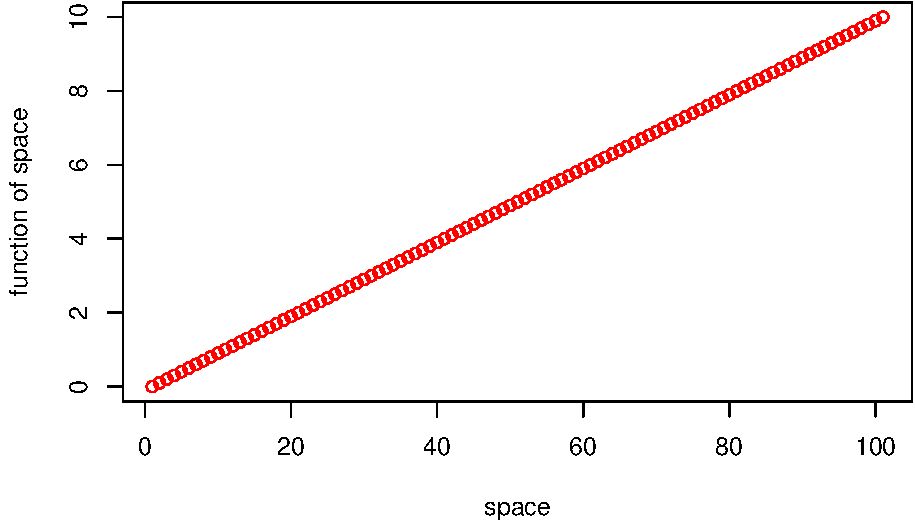
\includegraphics{foundational_statistics_files/figure-latex/unnamed-chunk-36-1.pdf}

We only supplied the one vector (\texttt{seq\_1}) to \texttt{plot()} in this case, which resulted in the function just defining the x-axis values as the numeric positions (1 to 101) of \texttt{seq\_1}. Also, this style of plot is known as a ``scatterplot.'' There is usually more ``scatter,'' for example when plotting two variables that not perfectly related. With \texttt{plot()}, we usually want to examine the relationship between two different variables, like below:

\begin{Shaded}
\begin{Highlighting}[]
\NormalTok{seq_}\DecValTok{1}\NormalTok{ <-}\StringTok{ }\KeywordTok{seq}\NormalTok{(}\FloatTok{0.0}\NormalTok{, }\FloatTok{10.0}\NormalTok{, }\DataTypeTok{by =} \FloatTok{0.1}\NormalTok{)}
\NormalTok{seq_}\DecValTok{2}\NormalTok{ <-}\StringTok{ }\KeywordTok{seq}\NormalTok{(}\FloatTok{10.0}\NormalTok{, }\FloatTok{0.0}\NormalTok{, }\DataTypeTok{by =} \FloatTok{-0.1}\NormalTok{)}
\KeywordTok{plot}\NormalTok{(seq_}\DecValTok{1}\NormalTok{, seq_}\DecValTok{2}\NormalTok{, }\DataTypeTok{xlab=}\StringTok{"sequence 1"}\NormalTok{, }\DataTypeTok{ylab =}\StringTok{"sequence 2"}\NormalTok{, }\DataTypeTok{type =} \StringTok{"p"}\NormalTok{, }\DataTypeTok{col =} \StringTok{"red"}\NormalTok{)}
\end{Highlighting}
\end{Shaded}

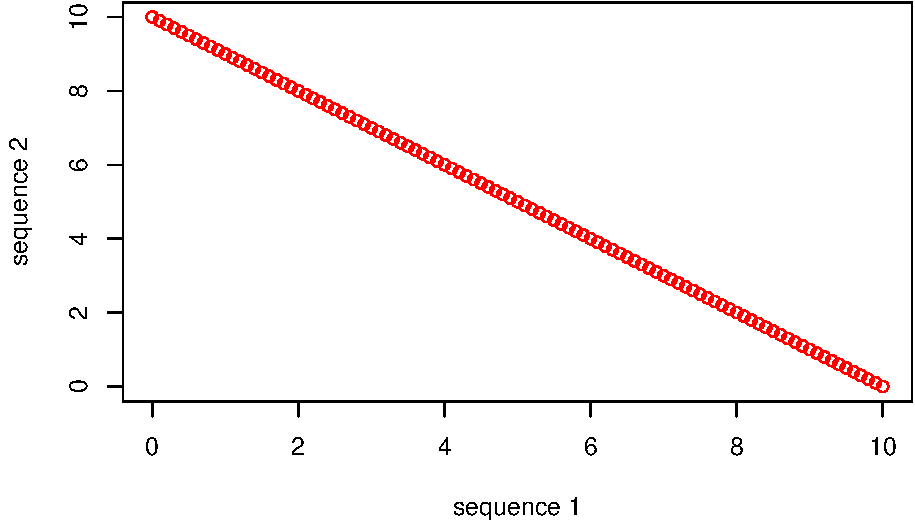
\includegraphics{foundational_statistics_files/figure-latex/unnamed-chunk-37-1.pdf}

In this example, \texttt{plot()} takes the first argument as the x-axis variable, and the second argument as the y-axis variable. You can also use the \texttt{\textasciitilde{}} to specify variables, but in this case the y-axis variable comes first (\texttt{y\ \textasciitilde{}\ x}). Also note the other arguments, which are usually named pretty intuitively. Note the axis label arguments, the type of object plotted (``p'' stands for ``points''), and the color of the plotted objects. There are many possible arguments, and many are actually set by another function called \texttt{par()}, that \texttt{plot()} calls on internally. One great resource for understanding plotting function arguments is the help menu for \texttt{par()}. I promise, if you become familiar with the \texttt{par()} documentation, you will quickly ascend the ranks of plotting prowess, and it will save you many frustrating moments in the future! I encourage you to study the \texttt{plot()} and \texttt{par()} documentation and practice using some of the other arguments that are especially useful, including ``main'', ``xlim'', ``ylim'', and ``cex'', for example.

The nice thing about graphical parameters is that, like many things in \texttt{R}, they are vectorized. So, if we want to use different symbols (look into the ``pch'' argument), colors (``col''), or sizes (look at ``cex'') of points for different observations in something like a data frame, we can supply those in the form of a vector! Taking the example above, if we want to plot the first 10 observations as blue, and the remaining observations as red, we can supply a vector of ``blues'' and ``reds'' in the appropriate order to \texttt{plot()}.

\begin{Shaded}
\begin{Highlighting}[]
\NormalTok{seq_}\DecValTok{1}\NormalTok{ <-}\StringTok{ }\KeywordTok{seq}\NormalTok{(}\FloatTok{0.0}\NormalTok{, }\FloatTok{10.0}\NormalTok{, }\DataTypeTok{by =} \FloatTok{0.1}\NormalTok{)}
\NormalTok{seq_}\DecValTok{2}\NormalTok{ <-}\StringTok{ }\KeywordTok{seq}\NormalTok{(}\FloatTok{10.0}\NormalTok{, }\FloatTok{0.0}\NormalTok{, }\DataTypeTok{by =} \FloatTok{-0.1}\NormalTok{)}
\KeywordTok{plot}\NormalTok{(seq_}\DecValTok{1}\NormalTok{, seq_}\DecValTok{2}\NormalTok{, }\DataTypeTok{xlab=}\StringTok{"sequence 1"}\NormalTok{, }\DataTypeTok{ylab =}\StringTok{"sequence 2"}\NormalTok{, }\DataTypeTok{type =} \StringTok{"p"}\NormalTok{, }
     \DataTypeTok{col =} \KeywordTok{c}\NormalTok{(}\KeywordTok{rep}\NormalTok{(}\StringTok{"blue"}\NormalTok{, }\DecValTok{10}\NormalTok{), }\KeywordTok{rep}\NormalTok{(}\StringTok{"red"}\NormalTok{, }\DecValTok{91}\NormalTok{)))}
\end{Highlighting}
\end{Shaded}

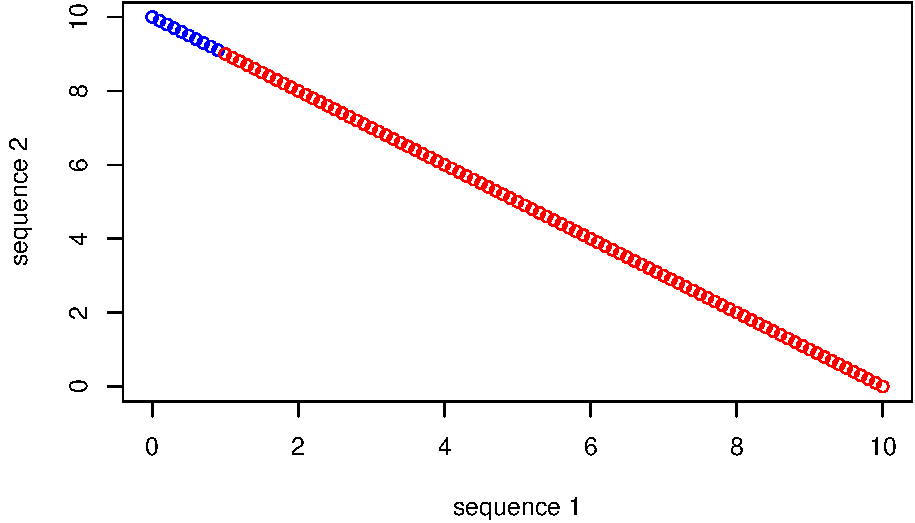
\includegraphics{foundational_statistics_files/figure-latex/unnamed-chunk-38-1.pdf}

You can see how this would be a nice way to differentiate among observation types in your data set, and produce an information-rich, single plot, as opposed to producing many plots that highlight single variables.

Sometimes we want to include multiple plots, as different panels, in the same figure. Fortunately this is made easy by the \texttt{mfrow} argument within \texttt{par()}. You simply set the dimensions, denoted by number of rows and number of columns in parentheses, before calling \texttt{plot()} repeatedly.

\begin{Shaded}
\begin{Highlighting}[]
\NormalTok{seq_square <-}\StringTok{ }\NormalTok{(seq_}\DecValTok{2}\NormalTok{)}\OperatorTok{*}\NormalTok{(seq_}\DecValTok{2}\NormalTok{)}
\NormalTok{seq_square_new <-}\StringTok{ }\NormalTok{(seq_}\DecValTok{2}\NormalTok{)}\OperatorTok{^}\DecValTok{2}

\KeywordTok{par}\NormalTok{(}\DataTypeTok{mfrow=}\KeywordTok{c}\NormalTok{(}\DecValTok{2}\NormalTok{,}\DecValTok{2}\NormalTok{))}
\KeywordTok{plot}\NormalTok{ (seq_}\DecValTok{1}\NormalTok{, }\DataTypeTok{xlab=}\StringTok{"time"}\NormalTok{, }\DataTypeTok{ylab =}\StringTok{"p in population 1"}\NormalTok{, }\DataTypeTok{type =} \StringTok{"p"}\NormalTok{, }\DataTypeTok{col =} \StringTok{'red'}\NormalTok{)}
\KeywordTok{plot}\NormalTok{ (seq_}\DecValTok{2}\NormalTok{, }\DataTypeTok{xlab=}\StringTok{"time"}\NormalTok{, }\DataTypeTok{ylab =}\StringTok{"p in population 2"}\NormalTok{, }\DataTypeTok{type =} \StringTok{"p"}\NormalTok{, }\DataTypeTok{col =} \StringTok{'green'}\NormalTok{)}
\KeywordTok{plot}\NormalTok{ (seq_square, }\DataTypeTok{xlab=}\StringTok{"time"}\NormalTok{, }\DataTypeTok{ylab =}\StringTok{"p2 in population 2"}\NormalTok{, }\DataTypeTok{type =} \StringTok{"p"}\NormalTok{, }\DataTypeTok{col =} \StringTok{'blue'}\NormalTok{)}
\KeywordTok{plot}\NormalTok{ (seq_square_new, }\DataTypeTok{xlab=}\StringTok{"time"}\NormalTok{, }\DataTypeTok{ylab =}\StringTok{"p in population 1"}\NormalTok{, }\DataTypeTok{type =} \StringTok{"l"}\NormalTok{, }\DataTypeTok{col =} \StringTok{'yellow'}\NormalTok{)}
\end{Highlighting}
\end{Shaded}

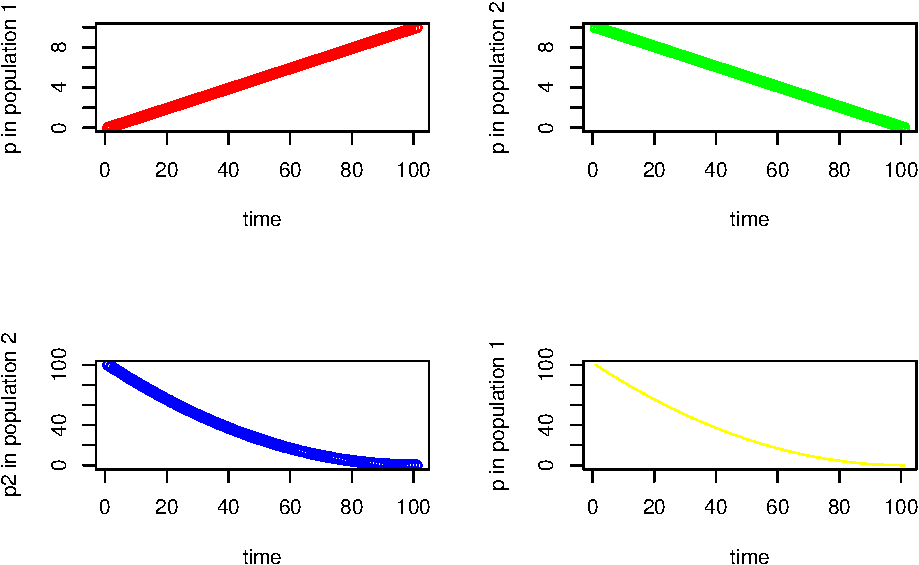
\includegraphics{foundational_statistics_files/figure-latex/unnamed-chunk-39-1.pdf}

\hypertarget{histograms-using-hist}{%
\subsection{\texorpdfstring{Histograms using \texttt{hist()}}{Histograms using hist()}}\label{histograms-using-hist}}

We will talk more about frequency distributions and histograms later in the course, but for now it is a good idea to become familiar with one way to plot them. If we have a quantitative variable, like height, and we want to know what the distribution among individuals looks like, we can use a histogram. The function \texttt{hist()} will help us with this task. To illustrate, below we will sample values from a binomial distribution. Don't worry about what this means now, as we will return to it later, but the scenario is intuitive. Let's say we flip a coin 20 times and record the number of ``heads'' as ``successes,'' and let's further say that we perform this ``20 coin flips'' activity 1000 times. And let's assume that our coin is ``fair,'' such that the probability of getting heads on any given flip is 0.5. We can simulate this process using the \texttt{rbinom()} function and plot the results using \texttt{hist()}.

\begin{Shaded}
\begin{Highlighting}[]
\KeywordTok{hist}\NormalTok{(}\KeywordTok{rbinom}\NormalTok{(}\DataTypeTok{n=}\DecValTok{1000}\NormalTok{, }\DataTypeTok{size=}\DecValTok{20}\NormalTok{, }\DataTypeTok{prob=}\FloatTok{0.5}\NormalTok{), }\DataTypeTok{xlab=}\StringTok{"number of heads"}\NormalTok{, }\DataTypeTok{ylab=}\StringTok{"number of activities"}\NormalTok{,}
     \DataTypeTok{main=}\StringTok{"Freq. Dist. of Coin Flip Successes"}\NormalTok{)}
\end{Highlighting}
\end{Shaded}

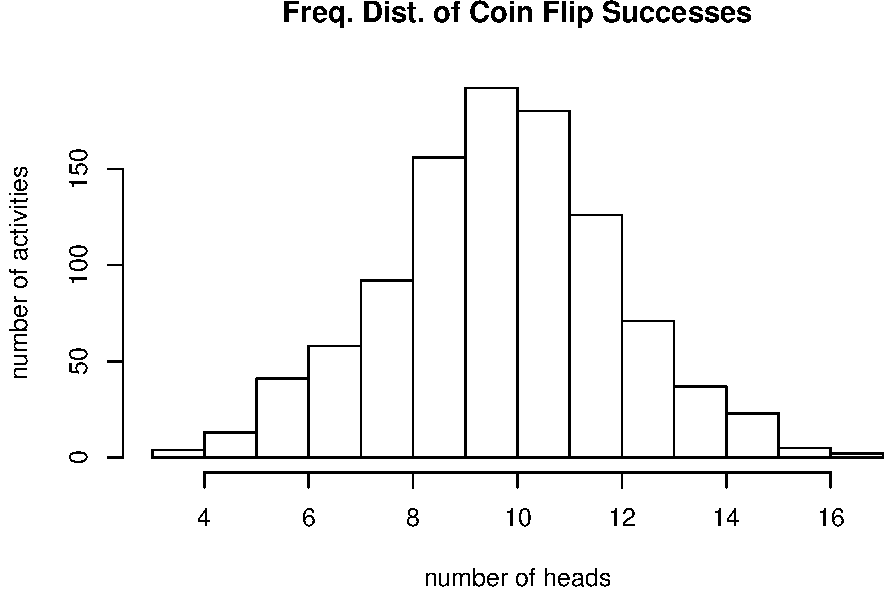
\includegraphics{foundational_statistics_files/figure-latex/binomial function-1.pdf}

Note that, as expected, our most frequent observation is that we get 10 heads out of 20 flips.

\hypertarget{boxplots-using-boxplot}{%
\subsection{\texorpdfstring{Boxplots using \texttt{boxplot()}}{Boxplots using boxplot()}}\label{boxplots-using-boxplot}}

In many cases we want to summarize the distribution of a qunatitiative variable using ``quartiles'' (we'll cover these in depth later), and perhaps we want to do this separately for different observation types in our data set. A boxplot (or ``box and whisker plot,'' depending on how it is drawn), depicts the 1st, 2nd (median), and 3rd quartile for a vector of numeric values using a box. ``Whiskers'' are often added to define ``fences'' beyond which are putative ``outliers.'' The \texttt{boxplot()} function of base \texttt{R} is convenient to use, particularly when your data set is organized in a data frame. Below is a series of simple examples to illustrate the utility of \texttt{boxplot()}

\begin{Shaded}
\begin{Highlighting}[]
\CommentTok{## make a modified version of the iris data frame, which includes a "Region" factor}
\NormalTok{new_iris <-}\StringTok{ }\NormalTok{iris}
\NormalTok{new_iris}\OperatorTok{$}\NormalTok{Region <-}\StringTok{ }\KeywordTok{as.factor}\NormalTok{(}\KeywordTok{rep}\NormalTok{(}\KeywordTok{c}\NormalTok{(}\KeywordTok{rep}\NormalTok{(}\StringTok{"West"}\NormalTok{, }\DecValTok{5}\NormalTok{), }\KeywordTok{rep}\NormalTok{(}\StringTok{"East"}\NormalTok{, }\DecValTok{5}\NormalTok{)), }\DecValTok{15}\NormalTok{))}

\CommentTok{## make a boxplot of Sepal.Length that plots individual boxes for the separate Species}
\KeywordTok{boxplot}\NormalTok{(Sepal.Length }\OperatorTok{~}\StringTok{ }\NormalTok{Species, }\DataTypeTok{data=}\NormalTok{new_iris)}
\end{Highlighting}
\end{Shaded}

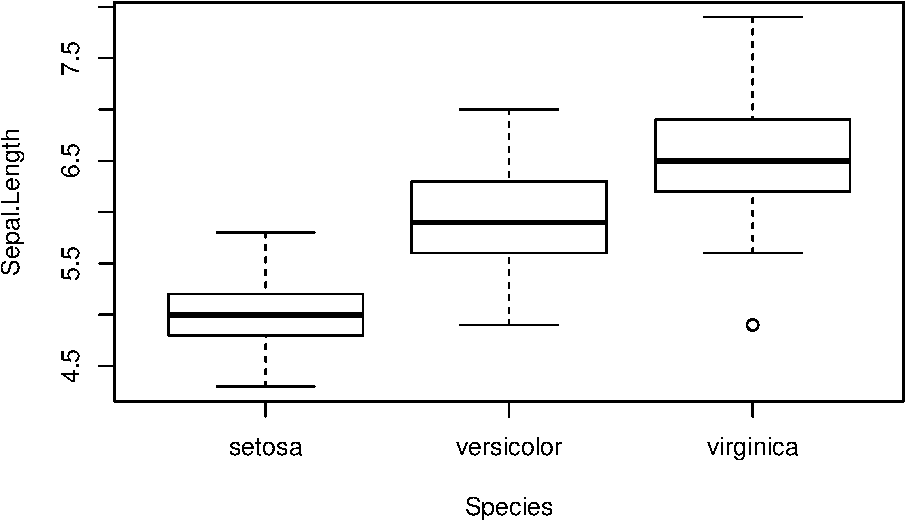
\includegraphics{foundational_statistics_files/figure-latex/unnamed-chunk-40-1.pdf}

\begin{Shaded}
\begin{Highlighting}[]
\CommentTok{## make a boxplot of Sepal.Length that shows all 6 combinations of factor levels from Species and Region, including a different color for each species}
\KeywordTok{boxplot}\NormalTok{(Sepal.Length }\OperatorTok{~}\StringTok{ }\NormalTok{Species}\OperatorTok{*}\NormalTok{Region, }\DataTypeTok{col=}\KeywordTok{c}\NormalTok{(}\StringTok{"blue"}\NormalTok{, }\StringTok{"red"}\NormalTok{, }\StringTok{"yellow"}\NormalTok{, }\StringTok{"blue"}\NormalTok{, }\StringTok{"red"}\NormalTok{, }\StringTok{"yellow"}\NormalTok{),}
        \DataTypeTok{data=}\NormalTok{new_iris, }\DataTypeTok{names=}\KeywordTok{c}\NormalTok{(}\StringTok{"set_E"}\NormalTok{,}\StringTok{"ver_E"}\NormalTok{,}\StringTok{"vir_E"}\NormalTok{,}\StringTok{"set_W"}\NormalTok{,}\StringTok{"ver_W"}\NormalTok{,}\StringTok{"vir_W"}\NormalTok{))}
\end{Highlighting}
\end{Shaded}

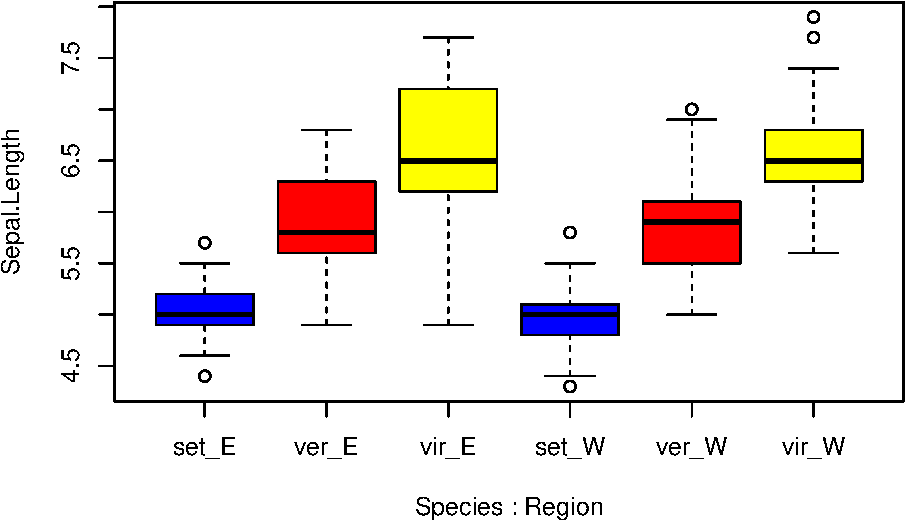
\includegraphics{foundational_statistics_files/figure-latex/unnamed-chunk-40-2.pdf}

Above you can see that by using the \texttt{*} character between the factors ``Species'' and ``Region in our plotting''formula" \texttt{boxplot()} produces a box for each factor level combination. Also, for \texttt{boxplot()} note that the ``col'' argument refers to the boxes themselves, so if we supply a vector of 6 colors, those will be applied to the boxes in order from left to right. Speaking of colors, an almost limitless array of colors can be specified in \texttt{R} plotting functions. Furthermore, colors can be coded using their names, or hexadecimal RGB specification. For a thorough treatment and great resources regarding colors in \texttt{R}, I recommend visiting the links at the bottom of the chapter.

\hypertarget{a-brief-introduction-to-rmarkdown}{%
\section{\texorpdfstring{A brief introduction to \texttt{RMarkdown}}{A brief introduction to RMarkdown}}\label{a-brief-introduction-to-rmarkdown}}

\texttt{RMarkdown} is a language that is distinct from \texttt{R}, but that incorporates \texttt{R} code ``chunks,'' which can be displayed and run if desired in the final, knitted output. The output can be knitted to a variety of file formats, such as \texttt{.html}, \texttt{.pdf}, or even Microsoft Word. For this course we will get into the habit of knitting to \texttt{.html}, which is the least buggy and error-prone in my experience. In the short section below, we will go over the simple steps required to write and knit your first \texttt{.Rmd} file, including the basic style elements of the language and some essential \texttt{R} chunk settings.

To get started using \texttt{RMarkdown}, you first need to make sure that you install the package \texttt{rmarkdown} from your Console, using \texttt{install.packages()}. Then, assuming you have an \texttt{RStudio} session running, click on File -\textgreater{} New File -\textgreater{} R Markdown. This will open a window in which you will type the name of your new file and the author's (your) name. A new file in your \texttt{RStudio} script editor pane (the upper left one) should appear. There will be a templated header, along with some other templated code, which you can modify based on your preferences. You may want to get rid of the pdf output line at the top for now, as we will knit to \texttt{.html} for this course. Knitting to \texttt{.pdf} requires some addtional software installation, which we don't have time to troubleshoot during this course. In any case, let's now cover some basic formatting code and code ``chunk'' types.

Below I will provide the code you would type in your own \texttt{RMarkdown} file, followed by what it looks like rendered in this \texttt{Bookdown} document, which is built using a collection of \texttt{RMarkdown} files itself!

\hypertarget{rmarkdown-formatting-basics}{%
\subsection{\texorpdfstring{\texttt{RMarkdown} formatting basics}{RMarkdown formatting basics}}\label{rmarkdown-formatting-basics}}

You can include ``nested'' headers (like the one directly above) by using \texttt{\#} symbols. For example this:

\begin{Shaded}
\begin{Highlighting}[]
\CommentTok{## Experiment with headers}

\CommentTok{### Try a third-level header}

\CommentTok{#### Or a fourth-level header}
\end{Highlighting}
\end{Shaded}

Renders as this:

\hypertarget{experiment-with-headers}{%
\section{Experiment with headers}\label{experiment-with-headers}}

\hypertarget{try-a-third-level-header}{%
\subsection{Try a third-level header}\label{try-a-third-level-header}}

\hypertarget{or-a-fourth-level-header}{%
\subsubsection{Or a fourth-level header}\label{or-a-fourth-level-header}}

Text can be rendered in bold, italics, or both like this:

\begin{Shaded}
\begin{Highlighting}[]
\ExtensionTok{Text}\NormalTok{ can easilly be *italicized* or **bolded** or ***both***}
\end{Highlighting}
\end{Shaded}

Which renders as this:

Text can easilly be \emph{italicized} or \textbf{bolded} or \textbf{\emph{both}}

Links can be included like this:

\begin{Shaded}
\begin{Highlighting}[]
\ExtensionTok{Here}\NormalTok{ is a useful link: [Rmd intro by RStudio](https://rmarkdown.rstudio.com/articles_intro.html)}

\ExtensionTok{Here}\NormalTok{ is another: [R Markdown cheat sheet](https://rmarkdown.rstudio.com/lesson-15.html)}
\end{Highlighting}
\end{Shaded}

Which render like this:

Here is a useful link: \href{https://rmarkdown.rstudio.com/articles_intro.html}{Rmd intro by RStudio}

Here is another: \href{https://rmarkdown.rstudio.com/lesson-15.html}{R Markdown cheat sheet}

For many more details on \texttt{RMarkdown} format and coding, I highly recommend the above links.

\hypertarget{rmarkdown-code-chunk-options}{%
\subsection{\texorpdfstring{\texttt{RMarkdown} code chunk options}{RMarkdown code chunk options}}\label{rmarkdown-code-chunk-options}}

Code chunks in \texttt{RMarkdown} exist to show \texttt{R} code, run the code, or both. In every \texttt{RMarkdown} file you write, you will demarcate code chunks with three ``ticks'' at the top of the chuck followed immediately by the chunk options in curly braces, on the same line, and another three ticks (on their own line) below the chunk of code. This is what a coded chunk looks like:

\begin{Shaded}
\begin{Highlighting}[]
\BaseNTok{```\{r, eval = TRUE, echo = TRUE\}}
\BaseNTok{seq(1, 10, 1)}
\BaseNTok{```}
\end{Highlighting}
\end{Shaded}

Which renders like this:

\begin{Shaded}
\begin{Highlighting}[]
\KeywordTok{seq}\NormalTok{(}\DecValTok{1}\NormalTok{, }\DecValTok{10}\NormalTok{, }\DecValTok{1}\NormalTok{)}
\end{Highlighting}
\end{Shaded}

\begin{verbatim}
##  [1]  1  2  3  4  5  6  7  8  9 10
\end{verbatim}

Note that in the above example the \texttt{R} code will be both run (``evaluated'') and displayed (``echoed'') in the knitted \texttt{.html} file. If we want to suppress either or both of those from being rendered, we just set the chunk options to ``FALSE''.

When your \texttt{RMarkdown} file is completed, save any final changes, and click on the ``Knit'' icon in the toolbar, or click File -\textgreater{} Knit Document. Assuming there are no errors in your code, the rendered \texttt{.html} file should load in a new window for inspection, and the file should be saved in the same location as your \texttt{.Rmd} file. This has been a minimal treatment of \texttt{RMarkdown}, but it should be enough guidance to get you started writing your own \texttt{RMarkdown} scripts. Please consult the aforementioned \texttt{RMarkdown} resources for additional instruction, examples, and help.

\hypertarget{exercises-associated-with-this-chapter-2}{%
\section{Exercises associated with this chapter:}\label{exercises-associated-with-this-chapter-2}}

\begin{itemize}
\tightlist
\item
  Exercise 2 (\texttt{rtutorial\_1} in \texttt{foundstats} R package)
\item
  Exercise 3 (\texttt{rtutorial\_2} in \texttt{foundstats} R package)
\end{itemize}

\hypertarget{additional-learning-resources-2}{%
\section{Additional learning resources:}\label{additional-learning-resources-2}}

\begin{itemize}
\item
  Logan, M. 2010. Biostatistical Design and Analysis Using R. - A great intro to R for statistical analysis
\item
  \url{http://library.open.oregonstate.edu/computationalbiology/} - O'Neil, S.T. 2017. A Primer for Computational Biology
\item
  \url{http://www.stat.columbia.edu/~tzheng/files/Rcolor.pdf} - A nice \texttt{.pdf} menu for many \texttt{R} colors
\item
  \url{https://www.stat.ubc.ca/~jenny/STAT545A/block14_colors.html} - A good introduction to colors in \texttt{R}
\item
  \url{https://medialab.github.io/iwanthue/} - A cool automated color palette selection tool
\item
  \url{https://rmarkdown.rstudio.com/articles_intro.html} - \texttt{RStudio} guide to \texttt{RMarkdown}
\item
  \url{https://rmarkdown.rstudio.com/lesson-15.html} - \texttt{RMarkdown} ``cheat sheet''
\end{itemize}

\hypertarget{introduction-to-probability-and-probability-distributions}{%
\chapter{Introduction to Probability and Probability Distributions}\label{introduction-to-probability-and-probability-distributions}}

\hypertarget{background-2}{%
\section{Background}\label{background-2}}

A practical knowledge of statistical inference requires a basic understanding of probability. For example we often want to understand how likely a particular observation or set of observations is (e.g.~from a sample of a population), given some expectation. That expectation may be based on a theoretical probability distribution we can use to model variation in nature. In this chapter we will introduce some core concepts of probability and how those pertain to understanding observed \textbf{parameters}, or features, and variation within systems.

\hypertarget{what-is-probability}{%
\section{What is probability?}\label{what-is-probability}}

\begin{itemize}
\tightlist
\item
  \textbf{Frequency interpretation}
  ``Probabilities are understood as mathematically convenient approximations to long run relative frequencies.''
\item
  \textbf{Subjective interpretation}
  ``A probability statement expresses the opinion of some individual regarding how certain an event is to occur.''
\end{itemize}

\hypertarget{random-variables-probability}{%
\section{Random variables \& probability}\label{random-variables-probability}}

\textbf{Probability} is the expression of belief in some future outcome based on information about a system. In statistics, we often think about variables we want to understand or estimate in the real world. In terms of probability, a \textbf{random variable} can take on different values with different probabilities. The \textbf{sample space} of a random variable is the universe of all possible values for that variable. It may be helpful to think of the sample space in the form of a plotted function, where possible values of the random variable make up the x-axis, and the probability of ``drawing'' a particular value at random makes up the y-axis.

The \textbf{sample space} can be represented by a \textbf{probability distribution} when our random variable is discrete. By discrete we mean that the variable can take on a limited (finite) number of values. Meristic traits like the number of bristles on the abdomen of an insect or the number of action potentials a neuron experiences in a single window of time can only have positive integer values. Continuous random variables like human height, on the other hand, can in theory take on an infinite number of values, but are in practice limited by our measurement precision. For continuous variables, the sample space is represented by what we call a \textbf{probability density function} (PDF). Probabilities over a sample space \textbf{always sum to 1.0}, and we use tools from algebra (for probability distributions) and calculus (for probability density functions) to make use of their properties in statistical modeling and inference.

Distributions of random variables can be expressed as functions that have \textbf{moments}. These moments are metrics of a function's shape, and these can be estimated. For example the 1st, 2nd, 3rd and 4th moments of a distribution correspond to the mean, variance, skewness, and kurtosis, respectrively. For now let's just consider the first two.

\begin{itemize}
\tightlist
\item
  The expectation or mean of a random variable X is:
\end{itemize}

\[E[X] = \sum_{\text{all x}}^{}xP(X=x) = \mu\]

\begin{itemize}
\tightlist
\item
  Often we want to know how dispersed the random variable is around its mean
\item
  One measure of dispersion is the variance:
\end{itemize}

\[Var(X) = E[X^2] = \sigma^2\]

There are many \textbf{families} or \textbf{forms} of probability distributions and PDFs, and which ones we apply in statistics depend on the dynamical system we are trying to represent. We will return to the most commonly used ones below. Probability distributions and PDFs are mathematically defined by features we call \emph{parameters}, which are defined by the moments pointed out above. The parameters of the functions themselves are used to understand properties of the systems we use the functions to model. For example the normal distribution (also called the Gaussian distribution), which is probably the most famous PDF in statistics, is characterized by 2 parameters: \(mu\) (the mean) and \(sigma^{2}\) (the variance). In practical terms, those parameters dictate the central peak or ``mode'' and the spread (width), respectively. These parameters are clearly important for us in thinking about the systems we study. For example in biology we often think about random variables as values expressed by individual living things. We may consider, in theory, all possible indviduals under a given set of circumstances, and one or more random variables associated with those individuals. In statistics we call this theoretical notion of all individuals a \textbf{\emph{population}}. If it makes sense to model a random variable in that population with a particular probability distribution or PDF, it opens the door to estimating the aforementioned parameters, but in the population. Mean height definitely tells us something about the most common values in a population of humans, as does how variable height is among individuals. So you can see how probability distributions and PDFs, when applied under the appropriate assumptions, help us understand, quantify, and compare random variables in populations.

\hypertarget{probability-and-the-bernoulli-distribution}{%
\section{Probability and the Bernoulli distribution}\label{probability-and-the-bernoulli-distribution}}

To think about probability and probability distributions, let's start with an example (the Bernoulli distribution. It describes the expected outcome of a single event with probability \texttt{p}. A good example of this scenario is the flipping of a \textbf{fair} coin once.

\[Pr(X=\text{Head}) = \frac{1}{2} = 0.5 = p \]

\[Pr(X=\text{Tails}) = \frac{1}{2} = 0.5 = 1 - p \]

\begin{itemize}
\item
  If the coin isn't fair then \(p \neq 0.5\)
\item
  However, the probabilities still sum to 1
  \[ p + (1-p) = 1 \]
  The same extensions can be made for other binary possibilities, like success or failure, ``yes'' or ``no'' answers, choosing an allele at a biallelic locus from a population, etc.
\end{itemize}

\hypertarget{probability-rules}{%
\section{Probability rules}\label{probability-rules}}

Let's take a moment to cover some basic rules of probability that have to do with observance of multiple ``events.''

\begin{itemize}
\tightlist
\item
  Let's say we flip a coin twice
\item
  Represent the first flip as `X' and the second flip as `Y'
\end{itemize}

\[ Pr(\text{X=H and Y=H}) = p*p = p^2 \]
\[ Pr(\text{X=H and Y=T}) = p*p = p^2 \]
\[ Pr(\text{X=T and Y=H}) = p*p = p^2 \]
\[ Pr(\text{X=T and Y=T}) = p*p = p^2 \]

\begin{itemize}
\tightlist
\item
  What about the probability that the \texttt{H} and \texttt{T} can occur in any order?
\end{itemize}

\[ \text{Pr(X=H and Y=T) or Pr(X=T and Y=H)} = \]
\[ (p*p) + (p*p) = 2p^{2} \]

\begin{itemize}
\tightlist
\item
  These are the \textbf{`and'} and \textbf{`or'} rules of probability

  \begin{itemize}
  \tightlist
  \item
    `and' means multiply the probabilities
  \item
    `or' means sum the probabilities
  \item
    most probability distributions can be built up from these simple rules
  \end{itemize}
\end{itemize}

\hypertarget{joint-probability}{%
\section{Joint probability}\label{joint-probability}}

\[Pr(X,Y) = Pr(X) * Pr(Y)\]\\

\begin{itemize}
\tightlist
\item
  Again (as above) this multiplication is true for two \textbf{independent} events
\item
  However, for two non-independent events we also have to take into account their \textbf{covariance}
\item
  To do this we need \textbf{conditional probabilities}
\end{itemize}

\hypertarget{conditional-probability}{%
\section{Conditional probability}\label{conditional-probability}}

\begin{itemize}
\tightlist
\item
  For two \textbf{independent} variables
\end{itemize}

\[Pr(Y|X) = Pr(Y)\text{ and }Pr(X|Y) = Pr(X)\]

\begin{itemize}
\tightlist
\item
  For two \textbf{non-independent} variables
\end{itemize}

\[Pr(Y|X) \neq Pr(Y)\text{ and }Pr(X|Y) \neq Pr(X)\]

Variables that are non-independent have a shared variance, which is also known as the \textbf{covariance}. You can think of this as two variables that consistently deviate from their respective meansCovariance standardized to a mean of zero and a unit standard deviation is \textbf{correlation} We will explore

\hypertarget{a-brief-note-on-likelihood-vs.probability}{%
\section{A brief note on likelihood vs.~probability}\label{a-brief-note-on-likelihood-vs.probability}}

\begin{itemize}
\item
  The \textbf{probability} of an event is the proportion of times that the event would occur if we repeated a random trial over and over again under the same conditions.
\item
  The \textbf{likelihood} is the probability of observing a particular set of data or outcome, given a particular parameter value.
\end{itemize}

\texttt{L{[}parameter\textbar{}data{]}\ =\ Pr{[}data\textbar{}parameter{]}}

Extending from this, the parameter value at which the likelihood is maximized is called the maximum likelihood estimate (MLE). You don't need to worry too much about likelihood in this course, but realize that many of our formualae for estimating parameters from data actually produce maximum likelihood estimates. The formula we use to calculate a mean from a sample of observations, for example, produces the maximum likelihood estimate for the population mean from which that sample was taken. The \textbf{likelihood function} (for a single parameter) or \textbf{likelihood surface} (for multiple parameters) describes the relationship between different parameter values and their likelihood. We can't always derive convenient equations to obtain maximum likelihood estimates, however, and in those cases we may have to rely on algorithmic searches of ``parameter space'' to find the MLE.

\hypertarget{probability-distributions-commonly-used-in-biological-statistics}{%
\section{Probability distributions commonly used in biological statistics}\label{probability-distributions-commonly-used-in-biological-statistics}}

(Many of these are thanks to Sally Otto at UBC)

\hypertarget{discrete-probability-distributions}{%
\subsection{Discrete Probability Distributions}\label{discrete-probability-distributions}}

\hypertarget{geometric-distribution}{%
\subsubsection{\texorpdfstring{\textbf{Geometric Distribution}}{Geometric Distribution}}\label{geometric-distribution}}

\begin{itemize}
\tightlist
\item
  If a single event has two possible outcomes the probability of having to observe \texttt{k} trials before the first ``one'' appears is given by the \textbf{geometric distribution}
\item
  The probability that the first ``one'' would appear on the first trial is \texttt{p}, but the probability that the first ``one'' appears on the second trial is \texttt{(1-p)*p}
\item
  By generalizing this procedure, the probability that there will be \texttt{k-1} failures before the first success is:
\end{itemize}

\[P(X=k)=(1-p)^{k-1}p\]

\begin{itemize}
\tightlist
\item
  mean = \(\frac{1}{p}\)
\item
  variance = \(\frac{(1-p)}{p^2}\)
\end{itemize}

\hypertarget{geometric-distribution-1}{%
\subsubsection{\texorpdfstring{\textbf{Geometric Distribution}}{Geometric Distribution}}\label{geometric-distribution-1}}

\begin{itemize}
\tightlist
\item
  Example: If the probability of extinction of an endangered population is estimated to be 0.1 every year, what is the expected time until extinction?
\end{itemize}

\begin{center}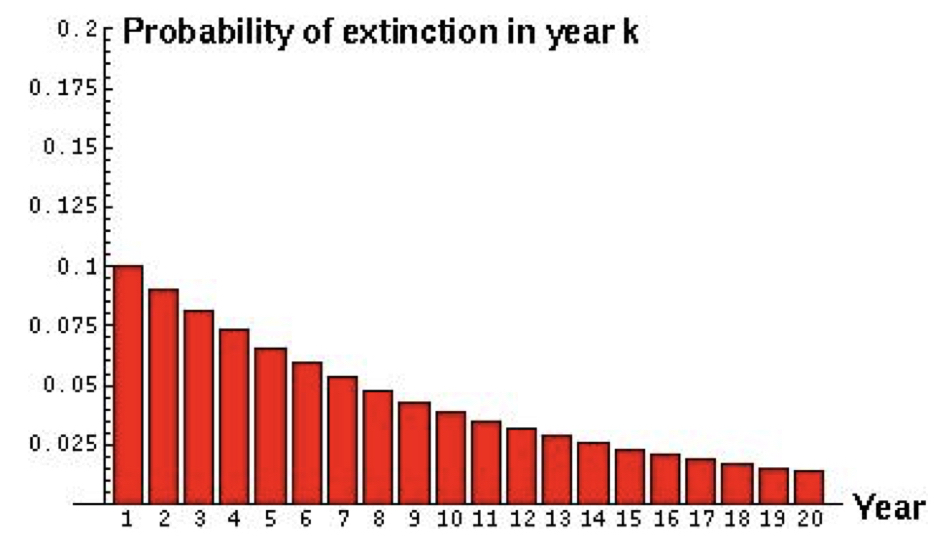
\includegraphics[width=0.8\linewidth]{images/prob.017} \end{center}

\hypertarget{binomial-distribution}{%
\subsubsection{\texorpdfstring{\textbf{Binomial Distribution}}{Binomial Distribution}}\label{binomial-distribution}}

\begin{itemize}
\item
  A \textbf{binomial distribution} results from the \textbf{combination} of several independent Bernoulli events
\item
  \textbf{Example}

  \begin{itemize}
  \tightlist
  \item
    Pretend that you flip 20 fair coins

    \begin{itemize}
    \tightlist
    \item
      or collect alleles from a heterozygote
    \end{itemize}
  \item
    Now repeat that process and record the number of heads
  \item
    We expect that most of the time we will get approximately 10 heads
  \item
    Sometimes we get many fewer heads or many more heads
  \end{itemize}
\item
  The distribution of probabilities for each combination of outcomes is
\end{itemize}

\[\large f(k) = {n \choose k} p^{k} (1-p)^{n-k}\]

\begin{itemize}
\tightlist
\item
  \texttt{n} is the total number of trials
\item
  \texttt{k} is the number of successes
\item
  \texttt{p} is the probability of success
\item
  \texttt{q} is the probability of not success
\item
  For binomial as with the Bernoulli \texttt{p\ =\ 1-q}
\end{itemize}

\begin{center}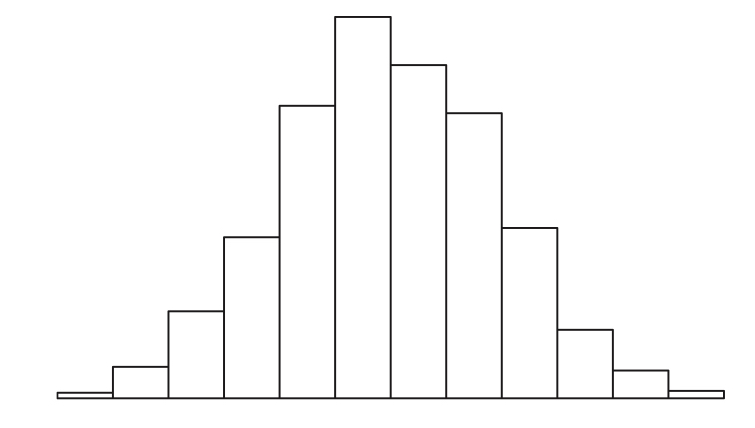
\includegraphics[width=1\linewidth]{images/week_2.003} \end{center}

\hypertarget{negative-binomial-distribution}{%
\subsubsection{\texorpdfstring{\textbf{Negative Binomial Distribution}}{Negative Binomial Distribution}}\label{negative-binomial-distribution}}

\begin{itemize}
\tightlist
\item
  Extension of the geometric distribution describing the waiting time until \texttt{r} ``ones'' have appeared.
\item
  Generalizes the geometric distribution
\item
  Probability of the \(r^{th}\) ``one'' appearing on the \(k^{th}\) trial:
\end{itemize}

\[P(X=k)=(\frac{k-1}{r-1})p^{r-1}(1-p)^{k-r}p\]

which simplifies to

\[P(X=k)=(\frac{k-1}{r-1})p^{r}(1-p)^{k-r}\]

\begin{itemize}
\item
  mean = \(\frac{r}{p}\)
\item
  variance = \(r(1-p)/p^2\)
\item
  Example: If a predator must capture 10 prey before it can grow large enough to reproduce
\item
  What would the mean age of onset of reproduction be if the probability of capturing a prey on any given day is 0.1?
\item
  Notice that the variance is quite high (\textasciitilde{}1000) and that the distribution looks quite skewed
\end{itemize}

\begin{center}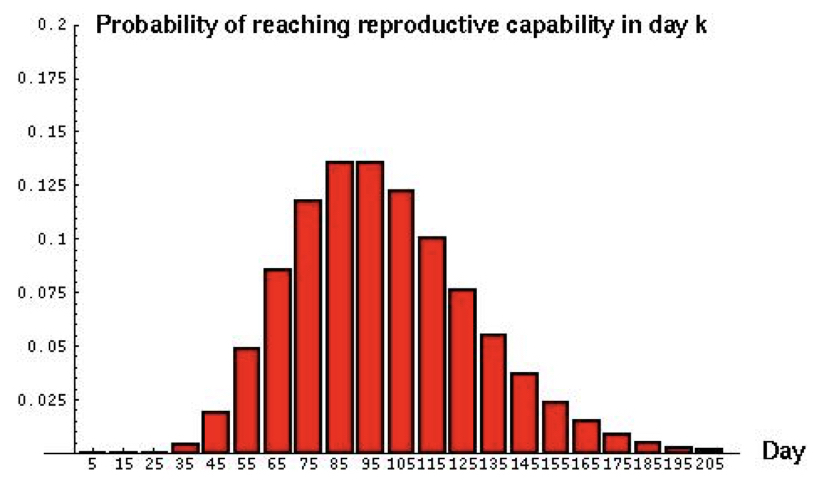
\includegraphics[width=0.5\linewidth]{images/prob.018} \end{center}

\hypertarget{poisson-probability-distribution}{%
\subsubsection{\texorpdfstring{\textbf{Poisson Probability Distribution}}{Poisson Probability Distribution}}\label{poisson-probability-distribution}}

\begin{itemize}
\item
  Another common situation in biology is when each trial is discrete, but the number of observations of each outcome is observed/counted
\item
  Some examples are

  \begin{itemize}
  \tightlist
  \item
    counts of snails in several plots of land
  \item
    observations of the firing of a neuron in a unit of time
  \item
    count of genes in a genome binned to units of 500 AA
  \end{itemize}
\item
  Just like before you have `successes', but

  \begin{itemize}
  \tightlist
  \item
    now you count them for each replicate
  \item
    the replicates now are units of area or time
  \item
    the values can now range from 0 to a large number
  \end{itemize}
\end{itemize}

\begin{itemize}
\tightlist
\item
  For example, you can examine 1000 genes

  \begin{itemize}
  \tightlist
  \item
    count the number of base pairs in the coding region of each gene
  \item
    what is the probability of observing a gene with `r' bp?
  \end{itemize}
\item
  \texttt{Pr(Y=r)} is the probability that the number of occurrences of an event \texttt{y} equals a count \texttt{r} in the total number of trials
\end{itemize}

\[Pr(Y=r) = \frac{e^{-\mu}\mu^r}{r!}\]

\begin{itemize}
\tightlist
\item
  Note that this is a single parameter function because \(\mu = \sigma^2\)
\item
  The two together are often just represented by \(\lambda\)
\end{itemize}

\[Pr(y=r) = \frac{e^{-\lambda}\lambda^r}{r!}\]

\begin{itemize}
\tightlist
\item
  This means that for a variable that is truly Poisson distributed:

  \begin{itemize}
  \tightlist
  \item
    the mean and variance should be equal to one another
  \item
    variables that are approximately Poisson distributed but have a larger variance than mean are often called `overdispersed'
  \item
    quite common in RNA-seq and microbiome data
  \end{itemize}
\end{itemize}

\hypertarget{poisson-probability-distribution-gene-length-by-bins-of-500-nucleotides}{%
\paragraph{Poisson Probability Distribution \textbar{} gene length by bins of 500 nucleotides}\label{poisson-probability-distribution-gene-length-by-bins-of-500-nucleotides}}

\begin{center}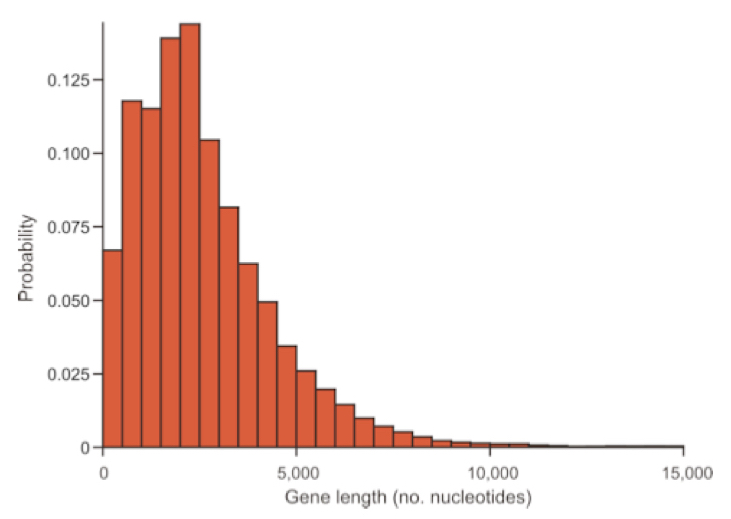
\includegraphics[width=0.8\linewidth]{images/week_2.004} \end{center}

\hypertarget{poisson-probability-distribution-increasing-parameter-values-of-lambda}{%
\paragraph{\texorpdfstring{Poisson Probability Distribution \textbar{} increasing parameter values of \(\lambda\)}{Poisson Probability Distribution \textbar{} increasing parameter values of \textbackslash{}lambda}}\label{poisson-probability-distribution-increasing-parameter-values-of-lambda}}

\begin{center}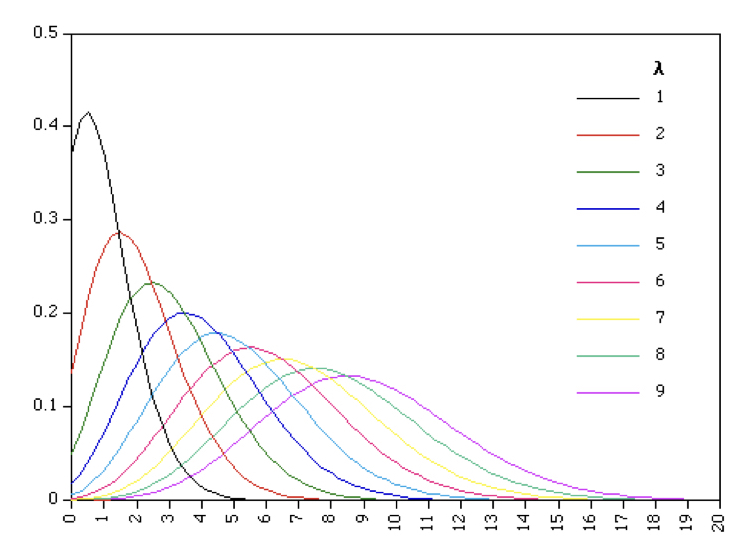
\includegraphics[width=0.7\linewidth]{images/week_2.005} \end{center}

\hypertarget{continuous-probability-distributions}{%
\subsection{\texorpdfstring{\textbf{Continuous probability distributions}}{Continuous probability distributions}}\label{continuous-probability-distributions}}

P(observation lies within dx of x) = f(x)dx

\[P(a\leq X \leq b) = \int_{a}^{b} f(x) dx\]

Remember that the indefinite integral sums to one

\[\int_{-\infty}^{\infty} f(x) dx = 1\]

\texttt{E{[}X{]}} may be found by integrating the product of \texttt{x} and the probability density function over all possible values of \texttt{x}:

\[E[X] = \int_{-\infty}^{\infty} xf(x) dx \]

\(Var(X) = E[X^2] - (E[X])^2\), where the expectation of \(X^2\) is

\[E[X^2] = \int_{-\infty}^{\infty} x^2f(x) dx \]

\hypertarget{uniform-distribution}{%
\subsubsection{\texorpdfstring{\textbf{Uniform Distribution}}{Uniform Distribution}}\label{uniform-distribution}}

\[E[X] = \int_{a}^{b} x\frac{1}{b-a} dx = \frac{(a+b)}{2} \]

\begin{center}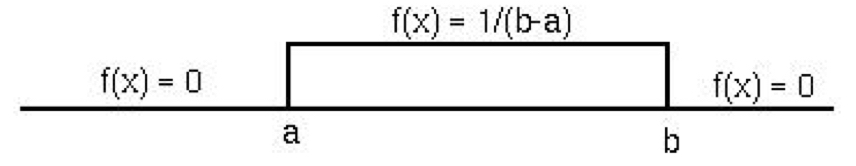
\includegraphics[width=1\linewidth]{images/prob.019} \end{center}

\hypertarget{exponential-distribution}{%
\subsubsection{\texorpdfstring{\textbf{Exponential Distribution}}{Exponential Distribution}}\label{exponential-distribution}}

\[f(x)=\lambda e^{-\lambda x}\]

\begin{itemize}
\tightlist
\item
  \texttt{E{[}X{]}} can be found be integrating \(xf(x)\) from 0 to infinity
\end{itemize}

\begin{itemize}
\tightlist
\item
  leading to the result that
\end{itemize}

\begin{itemize}
\item
  \(E[X] = \frac{1}{\lambda}\)
\item
  \(E[X^2] = \frac{1}{\lambda^2}\)
\item
  For example, let equal the instantaneous death rate of an individual.
\item
  The lifespan of the individual would be described by an exponential distribution (assuming that does not change over time).
\end{itemize}

\begin{center}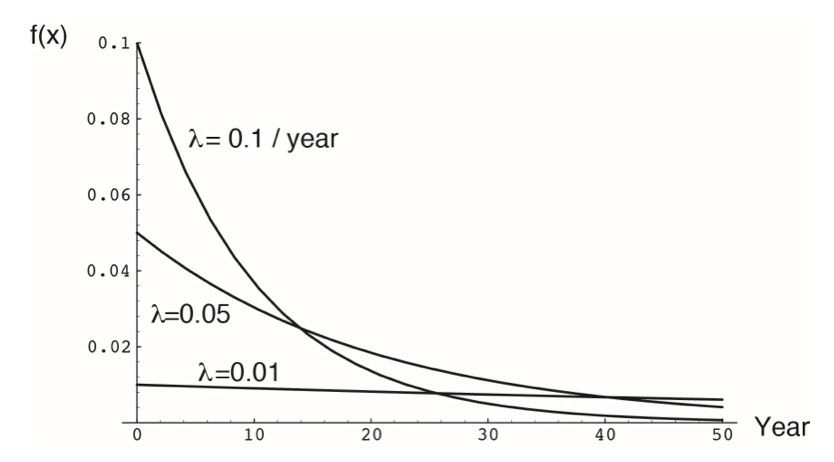
\includegraphics[width=0.7\linewidth]{images/prob.020} \end{center}

\hypertarget{gamma-distribution}{%
\subsubsection{\texorpdfstring{\textbf{Gamma Distribution}}{Gamma Distribution}}\label{gamma-distribution}}

\begin{itemize}
\tightlist
\item
  The gamma distribution generalizes the exponential distribution.
\item
  It describes the waiting time until the \(r^{th}\) event for a process that occurs randomly over time at a rate \(\lambda\) :
\end{itemize}

\[f(x) = \frac{e^{-\lambda x}\lambda x^{r-1}}{(r-1)!}\lambda\]

\[ Mean =  \frac{r}{\lambda} \]
\[ Variance = \frac{r}{\lambda^2} \]

\begin{itemize}
\tightlist
\item
  \textbf{Example}: If, in a PCR reaction, DNA polymerase synthesizes new DNA strands at a rate of 1 per millisecond, how long until 1000 new DNA strands are produced?
\end{itemize}

\begin{itemize}
\tightlist
\item
  Assume that DNA synthesis does not deplete the pool of primers or nucleotides in the chamber, so that each event is independent of other events in the PCR chamber.
\end{itemize}

\hypertarget{the-gaussian-or-normal-distribution}{%
\subsubsection{The Gaussian or Normal Distribution}\label{the-gaussian-or-normal-distribution}}

As mentioned, the normal distribution has two parameters.

\hypertarget{mu-and-sigma}{%
\paragraph{\texorpdfstring{(\(\mu\) and \(\sigma\))}{(\textbackslash{}mu and \textbackslash{}sigma)}}\label{mu-and-sigma}}

\begin{center}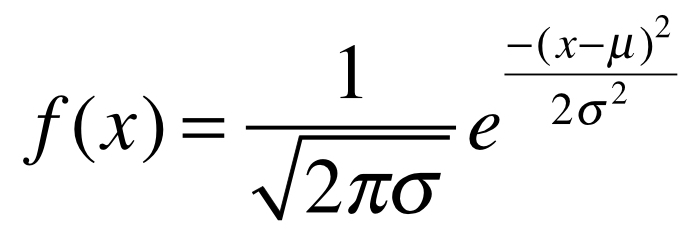
\includegraphics[width=0.4\linewidth]{images/week_2.032} \end{center}

where
\[\large \pi \approx 3.14159\]

\[\large \epsilon \approx 2.71828\]

To write that a variable (v) is distributed as a normal distribution with mean \(\mu\) and variance \(\sigma^2\), we write the following:

\[\large v \sim \mathcal{N} (\mu,\sigma^2)\]

\hypertarget{normal-pdf-estimates-of-mean-and-variance}{%
\paragraph{Normal PDF \textbar{} estimates of mean and variance}\label{normal-pdf-estimates-of-mean-and-variance}}

Estimate of the mean from a single sample

\[\Large \bar{x} = \frac{1}{n}\sum_{i=1}^{n}{x_i} \]

Estimate of the variance from a single sample

\[\Large s^2 = \frac{1}{n-1}\sum_{i=1}^{n}{(x_i - \bar{x})^2} \]

\begin{center}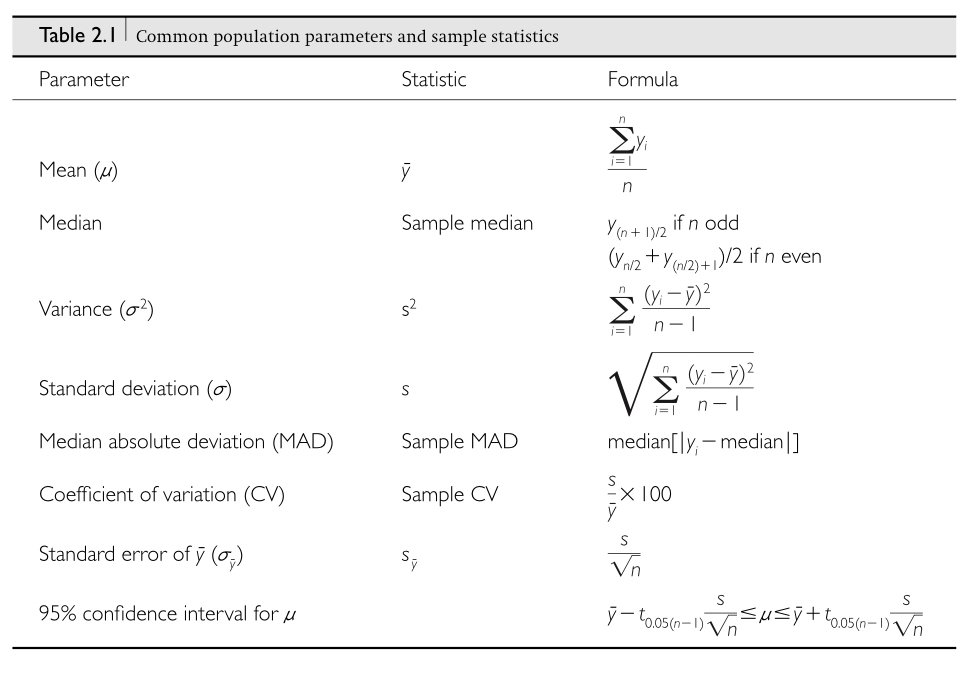
\includegraphics[width=0.9\linewidth]{images/week_2.010} \end{center}

\hypertarget{why-is-the-normal-special-in-biology}{%
\paragraph{Why is the Normal special in biology?}\label{why-is-the-normal-special-in-biology}}

\begin{center}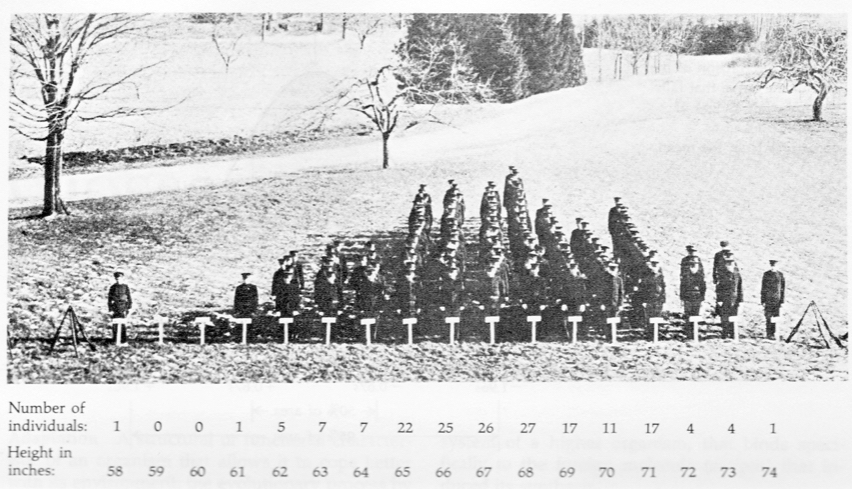
\includegraphics[width=1\linewidth]{images/week_2.013} \end{center}

\begin{center}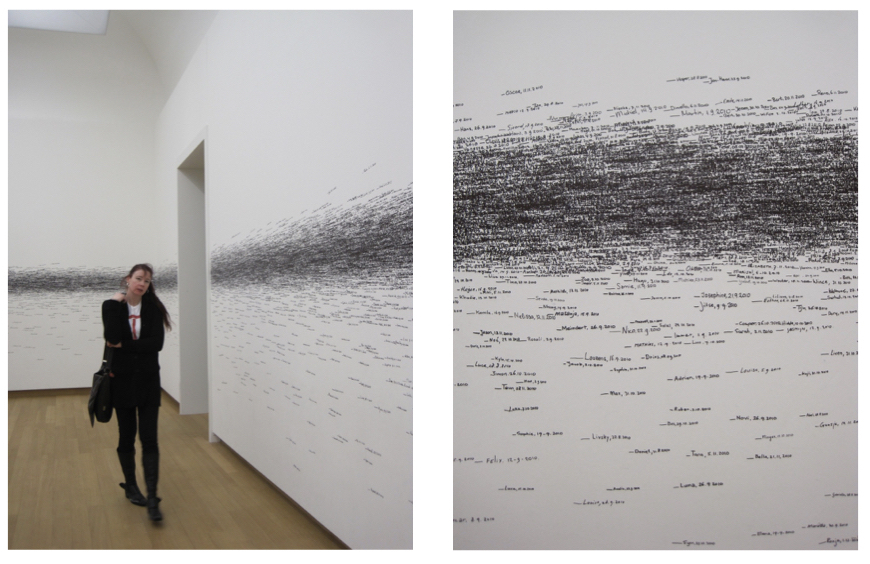
\includegraphics[width=1\linewidth]{images/week_2.015} \end{center}

\begin{center}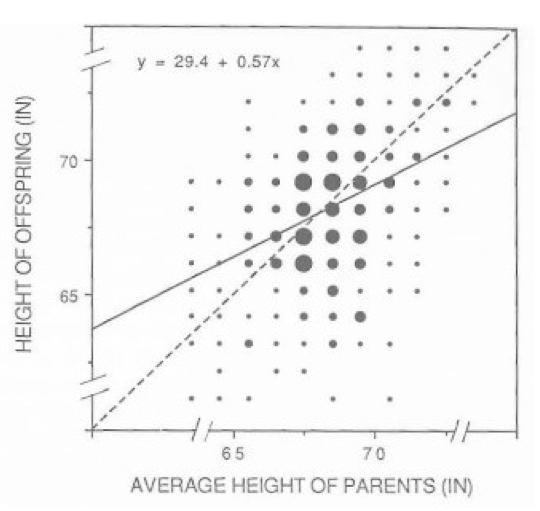
\includegraphics[width=0.6\linewidth]{images/week_2.014} \end{center}

\hypertarget{parent-offspring-resemblance}{%
\paragraph{Parent-offspring resemblance}\label{parent-offspring-resemblance}}

\begin{center}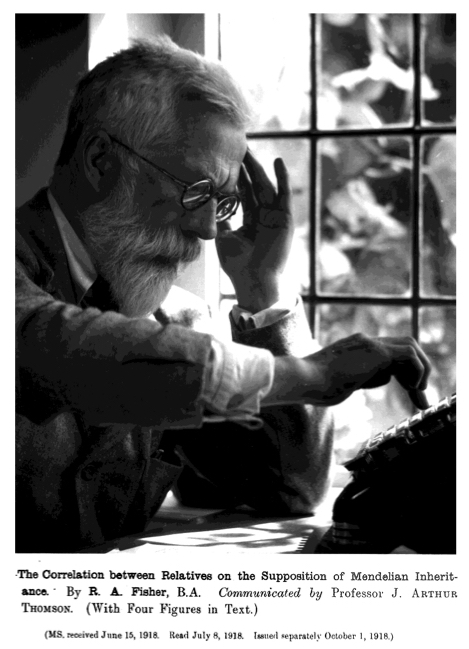
\includegraphics[width=0.45\linewidth]{images/week_2.016} \end{center}

\hypertarget{genetic-model-of-complex-traits}{%
\paragraph{Genetic model of complex traits}\label{genetic-model-of-complex-traits}}

\begin{center}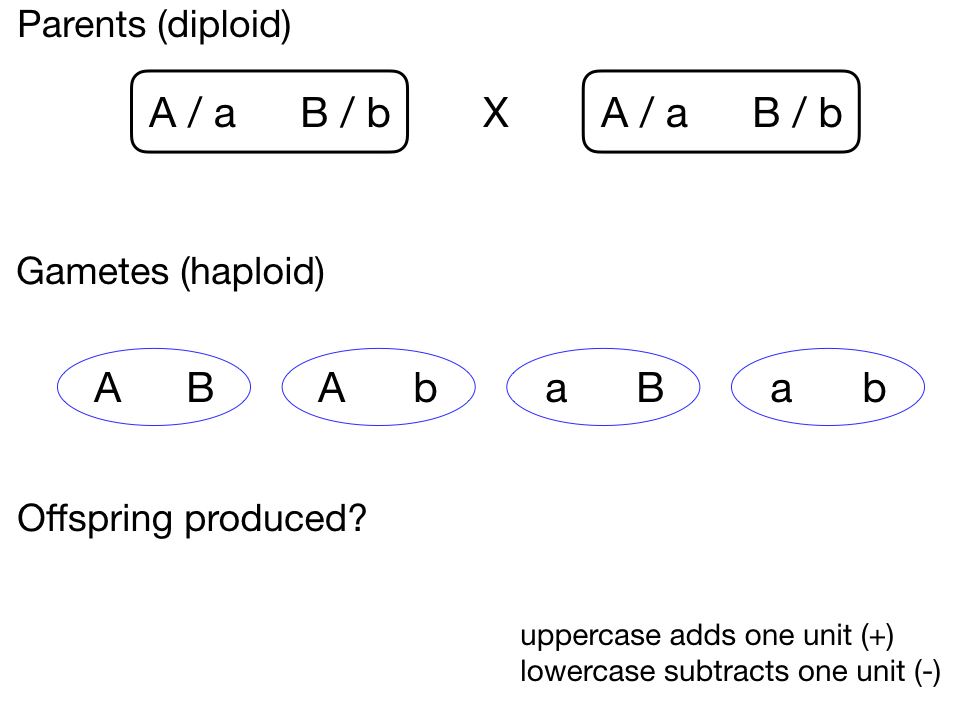
\includegraphics[width=0.9\linewidth]{images/week_2.017} \end{center}

\hypertarget{distribution-of-f_2-genotypes-really-just-binomial-sampling}{%
\paragraph{\texorpdfstring{Distribution of \(F_2\) genotypes \textbar{} really just binomial sampling}{Distribution of F\_2 genotypes \textbar{} really just binomial sampling}}\label{distribution-of-f_2-genotypes-really-just-binomial-sampling}}

\begin{center}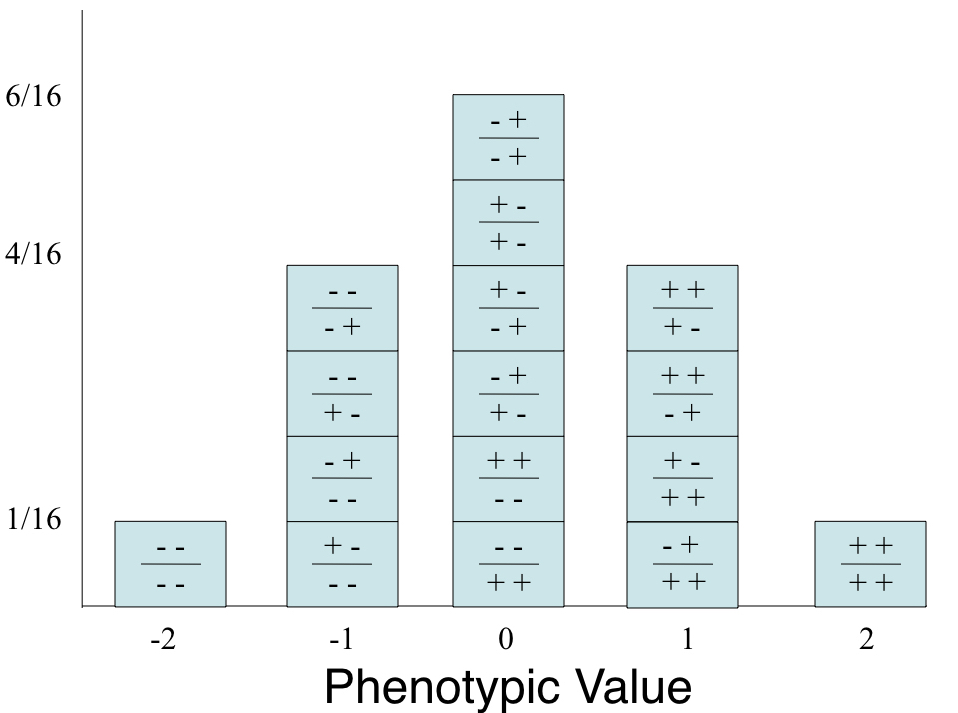
\includegraphics[width=0.7\linewidth]{images/week_2.018} \end{center}

\hypertarget{why-else-is-the-normal-special}{%
\paragraph{Why else is the normal special?}\label{why-else-is-the-normal-special}}

\begin{itemize}
\tightlist
\item
  The normal distribution is immensely useful because of the central limit theorem, which says that the he mean of many random variables independently drawn from the same distribution is distributed approximately normally
\item
  One can think of numerous situations, such as

  \begin{itemize}
  \tightlist
  \item
    when multiple genes contribute to a phenotype
  \item
    or that many factors contribute to a biological process
  \end{itemize}
\item
  In addition, whenever there is variance introduced by stochastic factors the central limit theorem holds
\item
  Thus, normal distributions occur throughout genomics
\item
  It's also the basis of the majority of classical statistics
\end{itemize}

\hypertarget{a-note-on-z-scores-of-normal-variables}{%
\paragraph{A note on z-scores of normal variables}\label{a-note-on-z-scores-of-normal-variables}}

\begin{itemize}
\tightlist
\item
  Often we want to make variables more comparable to one another
\item
  For example, consider measuring the leg length of mice and of elephants

  \begin{itemize}
  \tightlist
  \item
    Which animal has longer legs in absolute terms?
  \item
    Proportional to their body size?
  \item
    Proportional to their body size?
  \end{itemize}
\item
  A good way to answer these last questions is to use `z-scores'
\end{itemize}

\begin{itemize}
\tightlist
\item
  z-scores are standardized to a mean of 0 and a standard deviation of 1
\item
  We can modify any normal distribution to have a mean of 0 and a standard deviation of 1
\item
  Another term for this is the standard normal distribution
\end{itemize}

\[\huge z_i = \frac{(x_i - \bar{x})}{s}\]

\hypertarget{exercises-associated-with-this-chapter-3}{%
\section{Exercises associated with this chapter:}\label{exercises-associated-with-this-chapter-3}}

\begin{itemize}
\tightlist
\item
  Problem Set 2
\end{itemize}

\hypertarget{additional-learning-resources-3}{%
\section{Additional learning resources:}\label{additional-learning-resources-3}}

\begin{itemize}
\item
  Irizarry, R. A. Introduction to Data Science. \url{https://rafalab.github.io/dsbook/} - A gitbook written by a statistician, with great introductions to key topics in statistical inference.
\item
  Logan, M. 2010. Biostatistical Design and Analysis Using R. - A great intro to R for statistical analysis
\end{itemize}

\bibliography{book.bib,packages.bib}

\end{document}
